\PassOptionsToPackage{table,xcdraw}{xcolor}

\documentclass[sigconf,review,anonymous]{acmart}
\acmConference[ESEC/FSE 2023]{The 31st ACM Joint European Software Engineering Conference and Symposium on the Foundations of Software Engineering}{11 - 17 November, 2023}{San Francisco, USA}


\usepackage{booktabs}   %% For formal tables:
                        %% http://ctan.org/pkg/booktabs
\usepackage{subcaption} %% For complex figures with subfigures/subcaptions
                        %% http://ctan.org/pkg/subcaption
\usepackage{array}
\usepackage{amsmath,amsfonts}
\usepackage{algorithm}
\usepackage[noend]{algpseudocode}
%\usepackage{algorithmic}
\usepackage{graphicx}
\usepackage{textcomp}
\usepackage{float}
\usepackage{listings}
\usepackage{xspace}
\usepackage{multirow}
\usepackage{amsthm}
\newtheorem{definition}{Definition}
\usepackage{balance}

\usepackage[skins]{tcolorbox}

\usepackage{xcolor,pifont}
\newcommand*\colourcheck[1]{%
	\expandafter\newcommand\csname #1check\endcsname{\textcolor{#1}{\ding{52}}}%
}
\colourcheck{blue}
\colourcheck{green}
\colourcheck{red}

\newtcolorbox{myframe}[2][]{%
  enhanced,colback=white,colframe=black,coltitle=black,
  sharp corners,
  toprule=1.0pt,
  rightrule=0.3pt,
  leftrule=0pt,
  bottomrule=0pt,
  fonttitle=\itshape\scshape\large,
  left=0pt,right=5pt,top=5pt,bottom=3pt,
  attach boxed title to top right={yshift=-0.3\baselineskip-0.4pt,xshift=-5mm},
  boxed title style={tile,size=minimal,left=0.2mm,right=0.5mm,
    colback=white,before upper=\strut},
  title=#2,#1
}

%\newcommand{\code}[1]{{\footnotesize\textsf{#1}}}

\newcommand{\tool}{\textsc{CAT}\xspace}

\newcommand{\mvpdg}{$\delta$-PDG}

\newtheorem{Definition}{Definition}
\newtheorem{Claim}{Claim}
\newtheorem{Lemma}{Lemma}
\newtheorem{Theorem}{Theorem}

\newcolumntype{L}[1]{>{\raggedright\arraybackslash}p{#1}}
\newtheorem{observation}{Observation}
\newtheorem{property}{Property}
\newcommand{\code}[1]{{\footnotesize\texttt{#1}}}
\usepackage{amsthm}
 \definecolor{dkgreen}{rgb}{0,0.6,0}
\definecolor{gray}{rgb}{0.5,0.5,0.5}
\definecolor{mauve}{rgb}{0.58,0,0.82}
\lstset{frame=tb,
  language=Java,
  aboveskip=3mm,
  belowskip=3mm,
  showstringspaces=false,
  columns=flexible,
  basicstyle={\small\ttfamily},
  numbers=left,
  numberstyle=\tiny\color{gray},
  keywordstyle=\color{blue},
  commentstyle=\color{dkgreen},
  stringstyle=\color{mauve},
  breaklines=true,
  breakatwhitespace=true,
  tabsize=4
}

\newcommand{\mvpdgxy}{$\delta$-PDG$^{x,y}$}


\usepackage{tikz}
\usetikzlibrary{shapes.arrows}
\newcommand{\FancyUpArrow}{
\begin{tikzpicture}[baseline=-0.3em]
		\node[single arrow,draw,rotate=90,single arrow head extend=0.1em,inner
		ysep=0.1em,transform shape,line width=0.03em,top color=green,bottom color=green!50!black] (X){};
\end{tikzpicture}}

\begin{document}

%\title[{\tool}: Deep Fault Localization with Code Coverage Representation Learning]{{\tool}: Deep Fault Localization with Code Coverage Representation Learning}

\title[{\tool}: Context-aware, Graph-based, Commit-level Automated Vulnerability Detection and Assessment]{{\tool}: Context-aware, Graph-based, Commit-level Automated Vulnerability Detection and Assessment}


%%%---- AUTHORS BLOCK ------

\setcopyright{none}

\settopmatter{printacmref=false, printfolios=false}

\renewcommand\footnotetextcopyrightpermission[1]{} % removes footnote with conference information in first column


%(1) present information sorted in a way that a CNN can "see" patterns
%discriminating between faulty and non faulty statements more easily;

%(2) identify the actual crash statement to the network;

%(3) present more information to the deep neural network in the form of
%a summary of data dependences for each statement as well as source
%embedding; and

%(4) the suspiciousness of a statement is seen taking into account
%relationships to other statement, as opposed to a statement by itself”



%\input{sections/abstract}
\begin{abstract}
Software Vulnerabilities (SVs) are security weaknesses and flaws that
are exploitable in cyber-attacks. Delay in the assessment of SVs might
cause serious consequences due to the unknown impacts of the SVs on
the attacked systems. The state-of-the-art approaches have been proposed
to work directly on the code changes that were just committed to the
repository,
%Tien
%and deemed to have vulnerable code,
and detect any vulnerability and produce the assessment grades for
the detected one.
%Tien
%detected vulnerability.
However, those approaches still suffer low accuracy due to limited
representations for code changes and surrounding contexts.

We propose a Context-aware, Graph-based, Commit-level Vulnerability
Detection and Assessment Model, {\tool}, that evaluates a
%vulnerability-introducing
code change, detects any vulnerability and provides the CVSS
assessment grades for it. To build {\tool}, we have two~key novel
components. First, we design a novel context-aware, graph-based,
representation learning model to learn the {\em contextualized
embeddings for the code changes} that integrate program dependencies
and the surrounding contexts of code changes, facilitating the
learning to detect and assess the vulnerabilities.
%Those contextualized embeddings for code changes enable the
%learning to provide the CVSS assessment grades for the vulnerability.
Second, our automated assessment model,~during the assessment of one
security aspect, also considers the impacts of the other aspects by
leveraging multi-task learning (each~task learning to assess one
aspect) to propagate the learning from one task to another. Our
empirical evaluation shows that on a vulnerability dataset in C,
{\tool} achieves F-score of 25.5\% and MCC of 26.9\% relatively higher
than the state-of-the-art model in vulnerability
assessment. In a Java dataset, {\tool} achieves F-score of 20.4\% and
MCC of 28.0\% relatively higher as well.  It also improves the
vulnerability detection over the existing approaches.
%than DeepCVA in the assessment.
\end{abstract}


%\settopmatter{printacmref=true, printccs=true, printfolios=false}

%\begin{CCSXML}
%<ccs2012>
%<concept>
%<concept_id>10011007.10011006.10011073</concept_id>
%<concept_desc>Software and its engineering~Software maintenance tools</concept_desc>
%<concept_significance>500</concept_significance>
%</concept>
%</ccs2012>
%\end{CCSXML}

%\ccsdesc[500]{Software and its engineering~Software maintenance tools}

%\keywords{Deep Learning; Automated Program Repair; Context-based Code Transformation Learning}


\maketitle

\section{Introduction}
\label{intro:sec}

%The need for cyber resilience is increasingly important in our~techno\-logy-dependent society, where software systems have been, and will continue to be the target of cyber attackers.

Software Vulnerabilities (SVs) are security weaknesses and flaws that
are exploitable in the cyber-attacks. Vulnerability detection
models~\cite{li2018vuldeepecker,zhou2019devign,li2021sysevr} scan a
version of a software project and report any vulnerable code. It is
crucial to identify SVs as early as possible because late corrections
could cost much more and even cause severe damage due to more
affected systems. Toward that, {\em commit-level vulnerability
  detection} (VD)
approaches~\cite{perl2015vccfinder,zhou2017automated,chen2019large}
have been proposed to catch SVs as soon as new code changes are
committed to the code repositories during software development. They
are used to warn developers early on potential vulnerable code and
also help better prioritize the code review task.

%New software security vulnerabilities are discovered on an almost
%daily basis. It is crucial to identify software vulnerabilities as
%early as possible, because late corrections of errors could cost much
%more than early correction or even cause more severe
%damage. Recognizing this, researchers propose the approaches to detect
%software vulnerabilities as soon as new code changes are committed to
%the code repositories during software development. Those approaches
%are referred to as {\em commit-level vulnerability detection
%  (VD)}~\cite{perl2015vccfinder,zhou2017automated,chen2019large}. They
%could be used to warn developers early on potential vulnerable code.

For potential vulnerable code, it would be equally important to
provide developers with the assessment on the impacts of the detected
vulnerability on the system under development. The assessment could be
on the severity of the attack and the levels of damage regarding
confidentiality, integrity, availability, etc. However, the
commit-level VD
approaches~\cite{perl2015vccfinder,zhou2017automated,chen2019large} do
not support such automated assessment. Recognizing that importance,
the commit-level software vulnerability assessment (VA)
tools~\cite{deepCVA-ase21} have been proposed to assess a committed
code change. Researchers have leveraged the Common Vulnerability
Scoring System (CVSS) ratings~\cite{first-website} manually assessed
by security analysts for the vulnerabilities as labeled data to train
a machine learning (ML) model and applied it on the code change to
predict the assessment ratings. In CVSS, the security experts provide
the numerical scores that can be transformed into qualitative
representations (such as low, medium, high, and critical) for
vulnerability assessment. However, the state-of-the-art VA tools still
have key limitations.

First, the vulnerability assessment models~\cite{deepCVA-ase21} work
only on a committed change that was detected as vulnerable by a VD
tool. This strategy that runs VD and then VA (VD $\rightarrow$ VA)
would suffer the cascading error. For the false positive cases from
VD, the VA tool would give incorrect assessments, which should not be
given at all. Importantly, the VD $\rightarrow$ VA strategy would not
benefit from the {\em mutual impact between the learning of detection
  and the learning of assessment}. Our philosophy in this work is that
the detection and assessments of different aspects of a vulnerability
are interdependent on one another. If a model learns that one of the
assessment ratings is high (e.g., high severity or complete
unavailability), the vulnerability detection outcome must be
positive. If the detection outcome is negative, the assessment ratings
for all the aspects must be at the lowest (e.g., none). Thus, it is
more beneficial if a model learns both vulnerability detection and
assessment at the same time, leading to the performance improvement in
both tasks.

Second, the state-of-the-art VA approaches~\cite{deepCVA-ase21} are
still limited in the {\em representation of code changes} and do not
take into account the {\em context} of such changes. They use $n$-gram
representation for code changes that are insufficient to capture the
changed statements useful for the VD/VA but far apart. The statements
in an $n$-gram might not all contain important features for
VD/VA. $n$-grams also enforce an order in source code, which might not
be the execution order (e.g., in the cases of loop, condition, or
recursion), which is important to detect vulnerabilities involving
execution and exception flows. Moreover, for VD/VA, a model needs to
consider {\em program dependencies} among statements since an attack
to a vulnerability involves the exploits of the control and data
dependencies. With $n$-grams, the VA tools do not model the program
dependencies. Finally, it does not represent well the {\em code
  context} surrounding a change. The same change occurring in
different contexts might cause different effects, leading to different
impact grades. In the state-of-the-art VA tools, the context of
un-changed code is not distinguishable and not represented separately
from the code changes. The model can be confused by the two training
instances having the same combination of code changes and contexts,
but with different code changes and contexts themselves.

In this work, we present {\tool}, a Context-aware, Graph-based,
Commit-level Vulnerability Detection and Assessment Model to evaluate
a changed code, detect any vulnerability and provide the CVSS
assessment grades for the detected vulnerability. {\tool} provides
assessment scores when a vulnerability is detected. To build {\tool},
we provide a novel integration among three key ideas. First, we make
an {\bf integration of vulnerability detection and assessment (VDA)}
that could be built into a repository to evaluate the committed code
change to provide just-in-time assistance. Because the detection and
assessments of a vulnerability are interdependent, we leverage a {\bf
  multi-task learning} scheme to propagate the learning between VD and
VA, leading to better performance for both tasks. Moreover, the
assessments for different aspects could also affect one
another~\cite{deepCVA-ase21}, e.g., between the availability and
integrity of a system. Thus, our multi-task learning scheme includes
the VD task and all the assessment tasks for different security
aspects.

Second, regarding the code change representation, we develop a novel
{\em context-aware, graph-based, representation learning model} to
{\bf learn the contextualized embeddings for the code changes} that
integrate {\em program dependencies}, and the surrounding {\em
  contexts} of code changes.  Both versions of the program dependence
graphs (PDGs) before and after the commit are modeled via the
multi-version {\mvpdg}~\cite{flexeme-fse20}. To build such embeddings
for code changes, {\tool} {\em explicitly represents the contexts}
surrounding the changed statements via the sub-graphs in {\mvpdg}. It
considers the impact of the surrounding context represented by a
context vector on the building of the embeddings for the code
changes. {\tool} uses the contextualized embeddings to predict if the
changes have any vulnerability, and if yes, to provide assessment
grades. Third, we use the Label, Graph Convolution
Network~\cite{label-gcn} to encode the {\bf program dependencies}
among the entities in the changed code and the ones in the surrounding
un-changed code. This helps overcome the issues with $n$-grams and
capture the statements that might be far apart but are relevant to the
vulnerability.

%---------- OLD INTRO ----------------
%%%For potential vulnerable code, it would be also useful to provide
%%%developers with the assessment on the impacts of the vulnerability on
%%%the system under development. In the Common Vulnerability Scoring
%%%System (CVSS)~\cite{first-website}, the security experts and analysts
%%%have manually provided the assessments in terms of numerical ratings
%%%to quantify different aspects of a software vulnerability including
%%%the exploitability, the impacts and the severity of the attacks, the
%%%level of damages of the vulnerabilities,
%%%etc. (Figure~\ref{CVSS-tab}). The numerical scores can be transformed
%%%into qualitative representations (such as low, medium, high, and
%%%critical) to help organizations properly assess and prioritize their
%%%vulnerability management processes~\cite{first-website}. Despite its
%%%usefulness, there are restrictions. First, human efforts are needed
%%%for the {\em manual assessment}, leading to the delays in the process.
%%%Second, CVSS scores are provided {\em after} a vulnerability was
%%%reported. Thus, for an early action, an {\em automated, vulnerability
%%%  assessment} is desired at the committing time. The {\em
%%%  vulnerability detection and assessment tools (VDA)} can be
%%%integrated into the repositories as the code is checked in to provide
%%%just-in-time assistance.
%%%
%%%Recognizing such importance, the state-of-the-art, commit-level
%%%software vulnerability assessment tools~\cite{deepCVA-ase21} have been
%%%proposed to assess a committed code change. Researchers have leveraged
%%%the aforementioned CVSS ratings manually assessed by security analysts
%%%for the vulnerabilities as labeled data to train a machine learning
%%%(ML) model and applied it on the code change to predict the assessment
%%%ratings. However, none of the existing commit-level vulnerability
%%%assessment tools supports {\em both commit-level vulnerability
%%%  detection and assessment}. Importantly, they are still limited in
%%%the {\em representation of code changes} and do not take into account
%%%the {\em context} of such changes.
%%%
%%%Specifically, they are limited in using $n$-grams in representing code
%%%changes. $n$-grams are insufficient to capture the execution flows
%%%among code elements surrounding the changes. {\em The important
%%%  statements having dependencies with the changed statements can be
%%%  useful for the assessment, but can be far apart}. For example, many
%%%Denial of Service (DoS) vulnerabilities are related to null-pointer
%%%exceptions, exception flows, segmentation faults, etc. The execution
%%%flows among statements are not well-represented via $n$-grams with
%%%such limited lengths. Moreover, {\em the statements in an $n$-gram
%%%  might be irrelevant to the current vulnerability}. Thus, the
%%%assessment of a DoS vulnerability with $n$-grams could be
%%%imprecise. {\em $n$-grams also enforce an order in source code}, which
%%%might not be the execution order, e.g., in the cases of loop,
%%%condition, or recursion. The execution order and dependencies among
%%%the statements are important in an DoS. Thus, to assess the impact of
%%%a vulnerability, $n$-gram is limited.
%%%
%%%Second, to estimate the impacts of software vulnerability, a model
%%%needs to consider {\bf program dependencies} among statements since an
%%%attack to a vulnerability involves the~exploits of the control and
%%%data dependencies. The state-of-the-art vulnerability assessment tools
%%%capture code changes as code tokens in short sequences with $n$-grams,
%%%thus, does not model the program dependencies. Finally, it
%%%does not represent well the {\bf code context} surrounding a
%%%change. The same change occurring in different contexts might cause
%%%different effects, leading to different impact grades. In the
%%%state-of-the-art approaches~\cite{deepCVA-ase21}, the context of
%%%un-changed code is not~distinguishable and not represented
%%%separately from the code changes. The model can be confused by the two
%%%training instances having the same combination of code changes and
%%%contexts, but with different code changes and contexts
%%%themselves. Those limitations lead to low accuracy in the
%%%existing approaches.
%%%
%%%We present {\tool}, a Context-aware, Graph-based, Commit-level
%%%Vulnerability Detection and Assessment Model to evaluate a changed
%%%code, detect any vulnerability and provide the CVSS
%%%assessment grades for the detected vulnerability. To build {\tool}, we
%%%provide a novel integration among three key ideas. First, to make
%%%prediction on the CVSS assessment grades on code changes, we develop a
%%%novel {\bf context-aware, graph-based, representation learning
%%%  model} to {\bf learn the contextualized embeddings for the code
%%%  changes} that integrate {\em program dependencies}, and the
%%%surrounding {\em contexts} of code changes.  Both versions of the
%%%program dependence graphs (PDGs) before and after the commit are
%%%modeled via the multi-version {\mvpdg}~\cite{flexeme-fse20}.
%%%To build such embeddings for code changes, {\tool} {\em explicitly
%%%  represents the contexts} surrounding the changed statements via the
%%%sub-graphs in {\mvpdg}. It considers the impact of the surrounding
%%%context represented by a context vector on the building of the
%%%embeddings for the code changes. {\tool} uses the contextualized
%%%embeddings to predict if the changes have any vulnerability, and if
%%%yes, it provides assessment grades.
%%%
%%%Second, we use the Label, Graph Convolution
%%%Network~\cite{label-gcn} to encode the {\bf program dependencies}
%%%among the entities in the changed code and the ones in the
%%%surrounding un-changed code. This helps overcome the issues
%%%with $n$-grams and capture the statements that might be far
%%%apart but are relevant to the vulnerability.
%%%
%%%Third, the detection and assessments of different aspects of a
%%%vulnerability are interdependent on each other. For example, if a
%%%model learns one of the assessment ratings is high (e.g., high
%%%severity or complete unavailability), the vulnerability detection (VD)
%%%outcome must be positive. If the VD outcome is negative, the
%%%assessment ratings for all the aspects must be {\em none}. The
%%%assessments for different aspects could also affect one another, e.g.,
%%%between the availability and integrity of a system. Thus, we leverage
%%%a {\bf multi-task learning} model to propagate the learning from one
%%%task to another (each task learns to assess one aspect). Vulnerability
%%%detection is also a task in the multi-task learning scheme as {\tool}
%%%will provide assessment scores when a vulnerability is detected.

%-------------------------------------------------------------------------

%Experimental results
We have conducted experiments to evaluate {\tool} on real-world
vulnerabilities. Our results on a C vulnerability dataset
show that {\tool} achieves F-score of 25.5\% and MCC of 26.9\%
relatively higher than the state-of-the-art VA tool
DeepCVA~\cite{deepCVA-ase21}.  The vulnerability detection result from
{\tool} is also improved over the state-of-the-art ML/DL-based VD
approaches from 13.1-–157\% in precision, 15.8-–592\% in recall,
and 16.5–-350\% in F-score.
%approaches from 13.1-–29.8\% in precision, 15.8-–29.2\% in recall,
%and 16.5–-25.9\% in F-score.
The results on a Java dataset with 1,229 vulnerabilities show that
{\tool} achieves F-score of 31.0\% and MCC of 33.3\% relatively higher
than DeepCVA~\cite{deepCVA-ase21}.

%Our sensitivity analysis shows that all designed components in {\tool}
%contribute positively to its high accuracy.

For the insights, we conducted experiments to show that the better
performance of {\tool} roots from our designed components.
%We also conducted experiments to show that the higher~accuracy of
%{\tool} over DeepCVA comes from our designed~components.
Our results show that {\em our novel code change embeddings} help
{\tool} have better class-separation, i.e., better in classifying the
commits into the classes for vulnerability detection and
assessment. Moreover, we used {\em explainable AI} to show
that {\tool} indeed leverages the correct features in {\em program
  dependencies} among statements for its assessments.
The key contributions of this work include

{\bf 1. {\tool}: commit-level vulnerability detection and assessment
  model} that performs VD and VA in tandem, leveraging multi-task
learning to improve both detection and assessment.

%overcomes the issues in the existing model in $n$-gram representations
%of dependencies and contexts.

{\bf 2. Our novel context-aware, graph-based embeddings for code
  changes}
%Our {\em contextualized embeddings for code changes}
integrate dependencies and contexts. This embedding model
is applicable for other down-stream tasks.


{\bf 3. Empirical evaluation.} We evaluated {\tool}
against the state-of-the-art approach.
Our model/code are available at~\cite{cat-website}.



\section{Motivation}
\label{motiv:sec}

\subsection{Motivating Example}
\label{exe:sec}

%CVE-2021-37714: description
%CVSS Scores

%Input-Output

%Code Change: src/main/java/org/jsoup/parser/HtmlTreeBuilder.java

%Crash-point or infinite loop: HtmlTreeBuilderState.java

\begin{figure}[t]
  \begin{flushleft}
    \footnotesize
\textbf{Vulnerability Details: CVE-2021-37714}\\
\textbf{1. Description}:
{\em jsoup is a Java library for working with HTML. Those using jsoup versions prior to 1.14.2 to parse untrusted HTML or XML may be vulnerable to DOS attacks. If the parser is run on user supplied input, an attacker may supply content that causes the parser to get stuck (loop indefinitely until cancelled), to complete more slowly than usual, or to throw an unexpected exception. This effect may support a denial of service attack. The issue is patched in version 1.14.2. There are a few available workarounds. Users may rate limit input parsing, limit the size of inputs based on system resources, and/or implement thread watchdogs to cap and timeout parse runtimes.

  Publish Date : 2021-08-18 Last Update Date : 2022-02-07}

\textbf{2. Vulnerability Type(s)}: Denial Of Service

{\bf 3. CVSS Score:} ...\\

{\bf 4. Detailed CVSS Grades:}\\
\end{flushleft}
  \centering
  \tabcolsep 3pt
  \footnotesize
  \begin{tabular}{lll}
   Vulner. Assess. Type   & Value & Description \\
      \hline
    Confidentiality Impact & {\bf None}  & No impact to the confidentiality \\
    Integrity Impact & {\bf None}  & No impact to the integrity \\
    Availability Impact & {\bf Partial} & There is reduced performance or\\
    & & interruptions in availability\\
    Access Complexity & {\bf Low} & Specialized access conditions or \\
    & & extenuating circumstances do not exist\\
    & & Little knowledge is required to exploit\\
    Authentication & {\bf Not Req} & Authentication is not required \\
    & & to exploit the vulnerability\\
    Gained Access & {\bf None}  & No gained access with the vulnerability \\
    Acccess Vector & {\bf Local} & The vulnerability is in the local parser \\
    \end{tabular}%
  \label{CVSS:tab}%
\caption{Vulnerability Details: CVE-2021-37714}
\label{CVSS-tab}
\end{figure}

\begin{figure}[t]
	\centering
	\lstset{
		numbers=left,
		numberstyle= \tiny,
		keywordstyle= \color{blue!70},
		commentstyle= \color{red!50!green!50!blue!50},
		frame=shadowbox,
		rulesepcolor= \color{red!20!green!20!blue!20} ,
		xleftmargin=1.5em,xrightmargin=0em, aboveskip=1em,
		framexleftmargin=1.7em,
                numbersep= 5pt,
		language=Java,
    basicstyle=\scriptsize\ttfamily,
    numberstyle=\scriptsize\ttfamily,
    emphstyle=\bfseries,
                moredelim=**[is][\color{red}]{@}{@},
		escapeinside= {(*@}{@*)}
	}
	\begin{lstlisting}[]
// .../jsoup/parser/HtmlTreeBuilderState.java
boolean process(Token t, HtmlTreeBuilder tb) { ...
  if (t.isCharacter()&& inSorted( (*@{\color{red}{tb.currentElement().normalName()}@*),InTableFoster)){
     ...
     return tb.process(t);
  }
  ...
  } else {
      tb.popStackToClose(name);
(*@{\color{orange}{- \quad \quad tb.resetInsertionMode();}@*)
(*@{\color{orange}{- \quad \quad if (tb.state() == InTable) \{}@*)
(*@{\color{cyan}{+ \quad \quad if (!tb.resetInsertionMode()) \{}@*)
         tb.insert(startTag);
         return true;
      }
(*@{\color{red}{\quad \quad \quad return tb.process(t, InHead);}@*)
      ...
}
	\end{lstlisting}
        \vspace{-15pt}
        \caption{Code Change at Version 1.12.1 for CVE-2021-37714}
        \vspace{-6pt}
        \label{fig:motiv-code}
\end{figure}

%     tb.newPendingTableCharacters();
%     tb.markInsertionMode();
%     tb.transition(InTableText);

%A commit-level, vulnerability assessment tool takes as input a
%committed code change and estimates its impacts on the system under
%development with regards to confidentiality, integrity, availability,
%complexity, severity, etc. That code change might be deemed
%as vulnerable by a commit-level vulnerability detection tool.

Let us present an example from an HTML parser, named {\em jsoup}, and
our observations. Figure~\ref{CVSS-tab} displays the information on the
vulnerability CVE-2021-37714 that was reported on {\em jsoup}, and
published on 08/18/21. The change that was deemed to contribute to the
vulnerability were committed at version 1.12.1 to the method
\code{process(Token,HtmlTreeBuilder)} of the
\code{Html\-Tree\-Builder\-State} class (lines 10--11, and 12 of
Figure~\ref{fig:motiv-code}). That change directly uses the value
returned from \code{reset\-Inser\-tion\-Mode()} as the condition to
insert \code{starTag} (line 13). With this~change, certain input HTML
code with a specific start tag could make the program go to line 16
with a recursive call to the method \code{process(...)}. That~call
resulted in an NullPointerException at line 3 as noted in the
log:~{\em ``java.\-lang.\-Null\-Pointer\-Ex\-ception: Cannot invoke
  "org.\-jsoup.\-nodes.\-Element.\-normalName()" because the return
  value of
  "org.\-jsoup.\-parser.\-HtmlTree\-Builder.\-current\-Element()" is
  null.''}. In other cases, the parser can get stuck, i.e., {\em
  ``loop indefinitely until canceled''} as described in the official
description of CVE-2021-37714. Due
to those effects, this vulnerability is considered as {\em a denial of
  service (DoS)}. Figure~\ref{CVSS-tab} also shows the Common
Vulnerability Scoring System grades (CVSS) given by security experts
for various \underline{v}ulnerability \underline{a}ssessment
\underline{t}ypes (VATs) for CVE-2021-37714. Due to the above effects,
the availability impact for this vulnerability is rated as {\em
  Partial} (i.e., for some inputs, there will be reduced performance
and interruptions in available services).

While the above vulnerability potentially cause damages, both~the
detection and assessment for that vulnerability are late. That could
lead to more systems being affected by that vulnerability. Thus, it is
desirable to detect and assess a potential vulnerability as soon as
developers committed their vulnerable code to a repository during
software development. There exist the machine learning (ML) approaches
that automatically analyze the newly committed code, detect software
vulnerabilities~\cite{perl2015vccfinder,zhou2017automated,chen2019large}
and provide the assessments for them~\cite{deepCVA-ase21}. For
vulnerability assessment, those approaches have leveraged the manual
assessments from security analysts in CVSS to build labeled data to
train their ML models.
%Even though the CVSS system provides manual assessments after the
%vulnerabilities were detected/reported, the grades from security
%analysts actually are helpful as the labeled data for a machine
%learning (ML) to learn to automatically predict the gradings for a
%newly committed code change. In fact, DeepCVA~\cite{deepCVA-ase21}
%uses a $n$-gram representation with a ML model to learn from those
%manually assessments in CVSS to predict for a new commit.
A natural next question is what features in a code change are useful
for such an automated assessment. Toward answering that, from the
above example, we make the following observations.

%developed a machine learning (ML) model that learns from the existing
%grading from security experts to provide the new grading for a
%committed code change that was deemed to be vulnerable.  This type of
%commit-level automated vulnerability assessment together with a
%vulnerability detection (VD) tool are very useful in helping
%developers to early detect and assess the impacts of the detected
%vulnerability as soon as the code is committed. However, the
%state-of-the-art approach for commit-level vulnerability assessment
%is still limited as explained in the following observations.

\vspace{2pt}
\noindent {\bf Observation 1 [Program Dependencies].}  {\em To
  evaluate the impacts w.r.t. different VATs, a model needs to
  consider the program dependencies among the statements}. For
example, to assess Availability, one needs to check the potential
infinite loop or null-pointer exception, and examines the control and
data dependencies between the changed line 12 and the line 16. That is
where the method \code{process} is recursively called, which leads to
the null-pointer exception at line~3 (\code{currentElement()}
returns null). Unfortunately, the state-of-the-art vulnerability
assessment model, DeepCVA~\cite{deepCVA-ase21} with $n$-grams
($n$=1,3,5)
%to capture the surrounding code. $n$-grams are
is limited in capturing the dependencies in the surrounding code. The
important statements having the dependencies with the changed
statements can help with the assessment, but {\em can be far apart}
(e.g., line 12, line 16, and line 3). They cannot be well captured
with the $n$-grams of limited lengths of 1--5. The tokens within an
$n$-gram distance from the changed code might not be relevant to the
vulnerability. Moreover, $n$-grams require an order in source
code. However, the source code order might not reflect the execution~order. In Figure~\ref{fig:motiv-code}, line 12 has data/control flow to
line 16, which in turn has data/control flow to line 3 via recursion.


%The order should be on the dependency graph, rather than on source
%code.
\vspace{1pt}
\noindent {\bf Observation 2 [Context].} By examining {\em only the tokens
involving in the changes} (e.g., the tokens
\code{tb},~\code{reset\-Insertion\-Mode}, \code{state}, and \code{InTable}
in the deleted lines 10--11, and the inserted line 12), a model can
not decide if the vulnerability could have impact on the system's
availability or not.
%, i.e., deciding if the {\em Availability Impact}
%rating is {\em None}, {\em Partial}, or {\em Complete}.
Generally, {\em the same/similar changes occurring in different
  surrounding contexts might cause different effects, leading to
  different grades for the VATs}. For example, adding a null check:
\code{if p != null} is a common change in many places. However, it
could prevent a null-pointer exception in some context, while does not
in the others.
%(e.g., the availability impact in this case).
Unfortunately, DeepCVA~\cite{deepCVA-ase21} does not capture well the
contexts of the changes. First, it uses $n$-grams ($n$=1,3,5), which
is limited as explained. Second, DeepCVA does not explicitly
distinguish the context (un-changed code) from the changed code, which
confuses the model with two training instances having the same
context+code change, but with different code
changes or contexts. 

%do not explicitly modeling the context



\subsection{Key Ideas}
\label{key-ideas:sec}

We develop {\tool}, a Context-aware, Graph-based,
Commit-level~Vulnerability Detection and Assessment Model that detects
any vulnerability in a committed change and provides the CVSS
assessment grades for it if any.  {\tool} is designed with the
following ideas:

\vspace{1pt}
\indent {\bf Key Idea 1 [Multi-Task Learning among Vulnerability Detection
and Assessments]}. From Observation 1, we choose to leverage multi-task learning
to propagate the mutual benefits of learning of vulnerability
detection to vulnerability assessment, and vice versa. Moreover, the
learning of one type of vulnerability assessment could affect the
learning of the other (e.g., between Availability and Access
Complexity). Thus, our multi-task learning scheme is designed
with one task for VD, and one task for each of the assessment types. During training, we optimize the joint loss function for all the tasks. When the
VD's outcome is positive, {\tool} will provide the assessment
ratings. Otherwise, non-impact scores are given.

%If a model learns one of the assessment ratings is high (e.g.,
%complete unavailability), the VD outcome must be positive. If it is
%negative, the assessment ratings for all the aspects must be
%none. Morever, the learning of one aspect has impact on that of
%another one. Thus, we leverage multi-task learning to propagate such
%mutual learning. We consider the detection is one task of multi-task
%learning as when its outcome is positive, {\tool} will provide the
%assessment. Otherwise, non-impact scores are given.

\vspace{1pt}
\indent {\bf Key Idea 2 [Contextualized Embeddings for
Code Changes with Graph-based Representation Learning]}. To overcome
the limitation of code change representation, we introduce a
graph-based model to build the {\em
contextualized embeddings for code changes} that integrate both {\em
program dependencies} and {\em surrounding contexts}.

Unlike existing code change embedding
approaches~\cite{cc2vec,commit2vec} where code changes are represented
as sequences, we explicitly represent code changes and the
context of a change via a graph representation, called multi-version
PDG~\cite{flexeme-fse20}. The graph consists of
the program entities of both versions before and after the changes,
and their dependencies. The context is defined as the surrounding,
un-changed nodes of the changed node.
%
We use Label, Graph Convolution Network (Label-GCN)~\cite{label-gcn}
to build the contextualized embeddings for code changes, considering
the contexts as the weights in computation.
%
%The context vectors built from a Label, Graph Convolution Network
%(Label-GCN)~\cite{label-gcn} are then used as the weights representing
%the impacts of contexts in building the contextualized embeddings for
%code changes.
We use past vulnerabilities and experts' ratings to train {\tool}
to build such embeddings, and use them for classification.
%
%With such embeddings, we train {\tool} with the past vulnerabilities
%and human experts' ratings in CVSS to predict any vulnerability and
%its assessment.

%We train the Label-GCN~\cite{label-gcn} to learn the embeddings that
%are used in our automated assessment of the vulnerability types.


\vspace{1pt}
\indent {\bf Key Idea 3 [Program Dependencies in Code Change Representation
via Graph-based Neural Network]}.
%Graph-based Neural Network for
%Code Change Representation Learning of Program Dependencies]}.
We leverage Label-GCN~\cite{label-gcn} to incorporate the program dependencies among
the changed code elements and the surrounding un-changed code elements into {\tool}.
%
The graph enables a partial order among program entities in a PDG
rather than enforcing a total order as in $n$-gram learning.
%
This enables {\tool} overcome the aforementioned issues, 
%with $n$-grams 
and capture
dependencies on distant yet VDA-relevant statements.


%\vspace{1pt}
%\indent {\bf Key Idea 2 [Contextualized Embeddings for Code Changes].}
%We design a context-aware, graph-based, representation learning model
%to {\em learn the contextualized embeddings (vectors) for the code
%  changes} that integrate {\em program dependencies} among the program
%elements, and the {\em contexts} of~code changes. We train a
%Label-GCN~\cite{label-gcn} to learn the embeddings that are used in our
%automated assessment of the vulnerability assessment types (VATs).




\section{Approach Overview}
\label{overview:sec}

\begin{figure}[t]
	\centering
	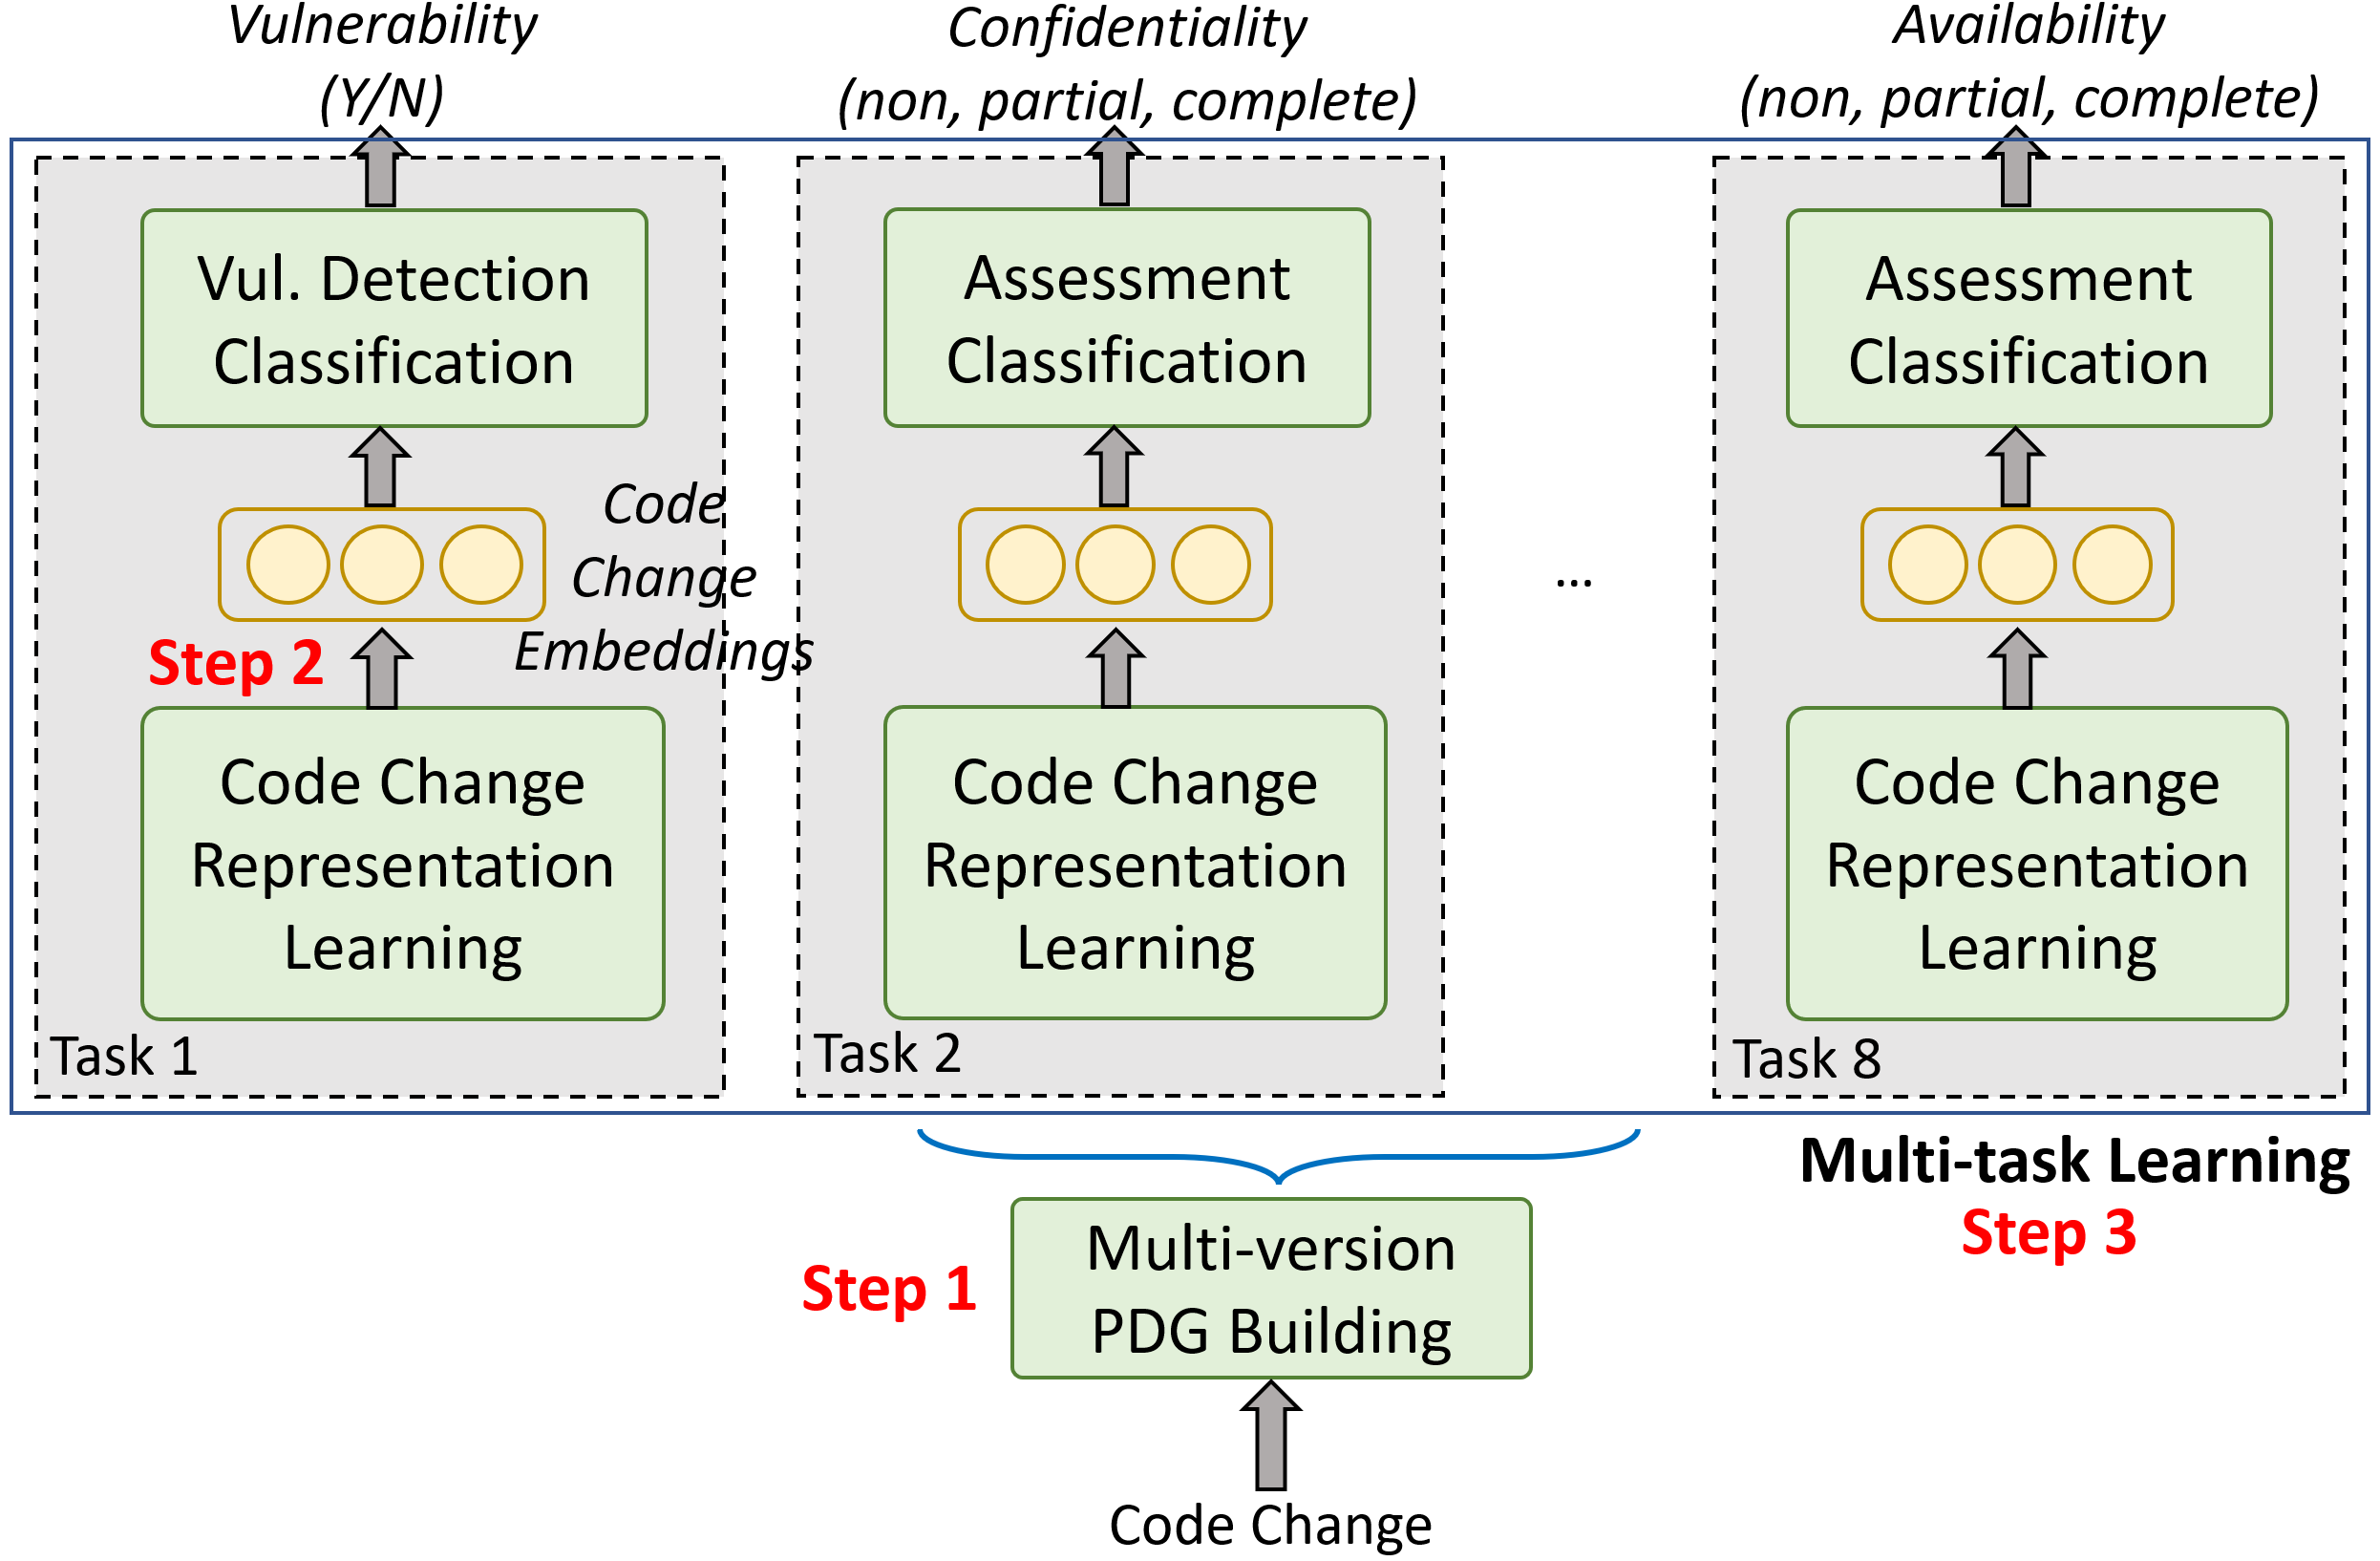
\includegraphics[width=3.4in]{graphs/overview-4.png}
	\vspace{-16pt}
	\caption{{\tool}: Context-aware, Graph-based, Commit-level
Vulnerability Detection and Assessment}
	\label{fig:overview}
\end{figure}

%Figure~\ref{fig:overview} illustrates the overall architecture of
%{\tool}.

\noindent {\tool} has three key components working in three~steps
(Figure~\ref{fig:overview}).

%\subsubsection*{{\bf Step 1. Multi-version PDG ({\mvpdgxy}) Generation}}

%\vspace{2pt}

\subsubsection*{{\bf Step 1. Representing Code Changes and Contexts with Multi-version PDG}}
Program Dependence Graph (PDG)~\cite{pdg} is a directed graph with a
set $N$ of nodes and a set $E$ of edges, in which a node $n \in N$
represents a program statement or a conditional expression; an edge $e
\in E$ represents the data or control flow among the statements.
%We adopt a graph representation, called
We adopt the multi-version PDG ({\mvpdgxy})~\cite{flexeme-fse20} to
represent the changes between two versions $x$ and $y$, before and
after the commit.  A multi-version PDG {\mvpdgxy}~\cite{flexeme-fse20}
is a directed graph generated from the disjoint union of all nodes and
edges in the PDGs at versions $x$ and~$y$. {\mvpdgxy}
(Figure~\ref{fig:multi-version-pdg}, Section~\ref{delta:sec}) allows
us to capture the program dependencies including data/control flows
that are crucial in vulnerability detection and assessment (Key
idea~2).

%\begin{Definition}[Multi-version Program Dependence Graph] ({\bf {\mvpdgxy}}).
%A {\mvpdgxy}~\cite{flexeme-fse20} is a directed graph generated from the
%disjoint union of all nodes and edges in the PDGs at versions $x$
%and~$y$.
%\end{Definition}

%{\mvpdgxy} is a directed graph generated from the disjoint union of
%all nodes and edges in both PDGs at the version $x$ and the version
%$y$ (Figure~\ref{fig:multi-version-pdg}).



%Contextualized Embeddings for Code Changes

%\vspace{2pt}

\subsubsection*{{\bf Step 2. Contextualized Embeddings for Code Changes with
    Graph-based Representation Learning}}
We develop our representation learning model to learn the
contextualized embeddings for the code changes in a commit that
integrate both program dependencies and the contexts. To build the
contextualized embeddings, we leverage the Label, Graph-based
Convolution Network~\cite{label-gcn} to learn the vector $v$ for each
node $n$ in the graph whose nodes can have labels. We use labels to
denote the nodes at either the versions $x$ (before changes) or $y$
(after changes), or at both versions.

For a changed node $n_c$, we collect all the un-changed nodes in the
context of $n_c$, which is defined as the set of all the un-changed
nodes that are $k$-hop neighbors of $n_c$. In
Figure~\ref{fig:multi-version-pdg}, for the changed statement at line
4, if $k=1$, the context of that change includes the statements at
lines 2, 5, and 7 (i.e., 1-hop neighbors from line 4).

From the context nodes, we compute the vector for the context for a
changed node $n_c$ and use it as a weight to represent the impact of
context to build the contextualized embedding for $n_c$.  From those
embeddings, we compute the vector for the entire commit and feed it to
a SoftMax layer acting as a classifier to perform vulnerability
classification or assessment classification for each assessment
type. The softmax function is often used as the last activation
function of a neural network to normalize the output of a network to a
probability distribution over the predicted output classes.

%Tien rewrote this para as above
%We collect the vectors of the context nodes into a matrix and use a
%fully connected layer to convert the matrix into a vector $v_{ctx}$ to
%encode the contextual information for the changed node $n_c$. The
%context vector $v_{ctx}$ is used as a weight to represent the impact
%of context on learning to build the contextualized embedding for the
%changed node $n_c$. We next concatenate all the vectors for the all
%the changed nodes $n_c$s into a matrix and use a fully connected layer
%to build the final vector $v^{com}$ for the entire commit. Finally, we
%feed the vector $v^{com}$ to a SoftMax layer acting as a classifier to
%perform assessment classification for each CVSS assessment type.


%\subsubsection{{\bf Step 2. Multi-task Learning-based Vulnerability Assessment Classification}}

%After having the {\mvpdgxy}, this step is mainly used to do the classification for seven different vulnerability assessment types. To achieve that, \tool setups seven separate but similar tasks on seven vulnerability assessment classification problems. Here, we pick one task to explain it in detail.

%The first step of the vulnerability assessment classification is to learn the summarized representation vector for the code changes in the vulnerability bring commit. In this step, \tool uses the Label-GCN \cite{} that can deal with the nodes with multiple labels (suitable for $x$, $y$, and $x,y$ labels in {\mvpdgxy})to learn the representation vector $v$ for each node $n$ in the graph. \tool then picks out all changed nodes in {\mvpdgxy} as a set. For each changed node $n^c$ in this set, \tool firstly collects the representation vector $v^{uc}$ for all unchanged nodes $n^{uc}$ within the $k$-hops in {\mvpdgxy} as the context of the changed node $n^c$. For example, in the {\mvpdgxy} in Figure \ref{fig:multi-version-pdg}, if we regard the statement in $line-4$ is the changed statement that we are focusing on. When $k=1$, the context of it includes the statements in $line-2$, $line-5$, and $line-7$. By concatenating $v^{uc}$ in a new dimension as a matrix, \tool uses a fully connected layer to summarize the matrix into one vector $v^{ctx}$ to represent the context information for the changed node $n^c$. Then, \tool uses the cross product to combine the node representation vector $v^c$ with the context representation vector $v^{ctx}$ to get the final representation vector $v'^c$ for the changed node $n^c$.


%Because the vulnerability assessment we want to get is for the whole vulnerability bring in commits, \tool concatenates $v'^c$ as a matrix and uses a fully connected layer to summarize the final code change representation vector $v^{commit}$. After having the final code change representation vector $v^{commit}$, \tool uses the SoftMax layer as a classifier to do the vulnerability assessment classification based on the $v^{commit}$.

%\vspace{2pt}
\subsubsection*{{\bf Step 3. Multi-Task Learning for Classification}}

For each assessment type, we~have a SoftMax layer working as an
assessment classification model on the embedding of the entire commit.
We also have another SoftMax layer as the classifier for
vulnerability detection.
%
%the SoftMax layer acts as the classifier, which takes
%the~contextualized embedding for the entire commit built on the
%{\mvpdgxy} and performs classifications.
%
To propagate the impact of the classification for one assessment type
on one another, we leverage multi-task learning among all the
classification models. We use the uncertainty weighted multi-task
loss~\cite{kendall2018multi} for each classification task as the final
multi-task learning loss function and use the maximum of the average
F-score from all the classification tasks as the training~target.

%After \tool has seven different classification tasks as we introduced above, \tool uses the weighted linear sum of the losses for each task as the final multi-task learning loss function and uses the maximum of the average F-1 score from all vulnerability assessment classification tasks as the training target to train the model.

%When making a prediction, based on the requirements, \tool can directly provide classification results for a single vulnerability assessment type or multiple vulnerability assessment types as needed.

%Training and Predicting process

\subsubsection*{{\bf Training and Predicting Processes}}
The training and predicting processes share the above steps, except
that in training, the classification labels for the vulnerable commit
and vulnerability assessment types (VATs) are known. For a benign
commit, the output labels are negative and non-impact.
%vulnerability-introducing commits w.r.t. a VAT are known.
When predicting, {\tool} takes a code change, predicts
vulnerability and provides the assessment classifications for seven
VATs. Next, we will explain {\tool} in details.

%directly provide classification results for a single vulnerability
%assessment type or multiple vulnerability assessment types as needed.


%fix the figure


\section{Building multi-version PDG ({\mvpdgxy})}
\label{delta:sec}

\begin{figure}[t]
	\centering
	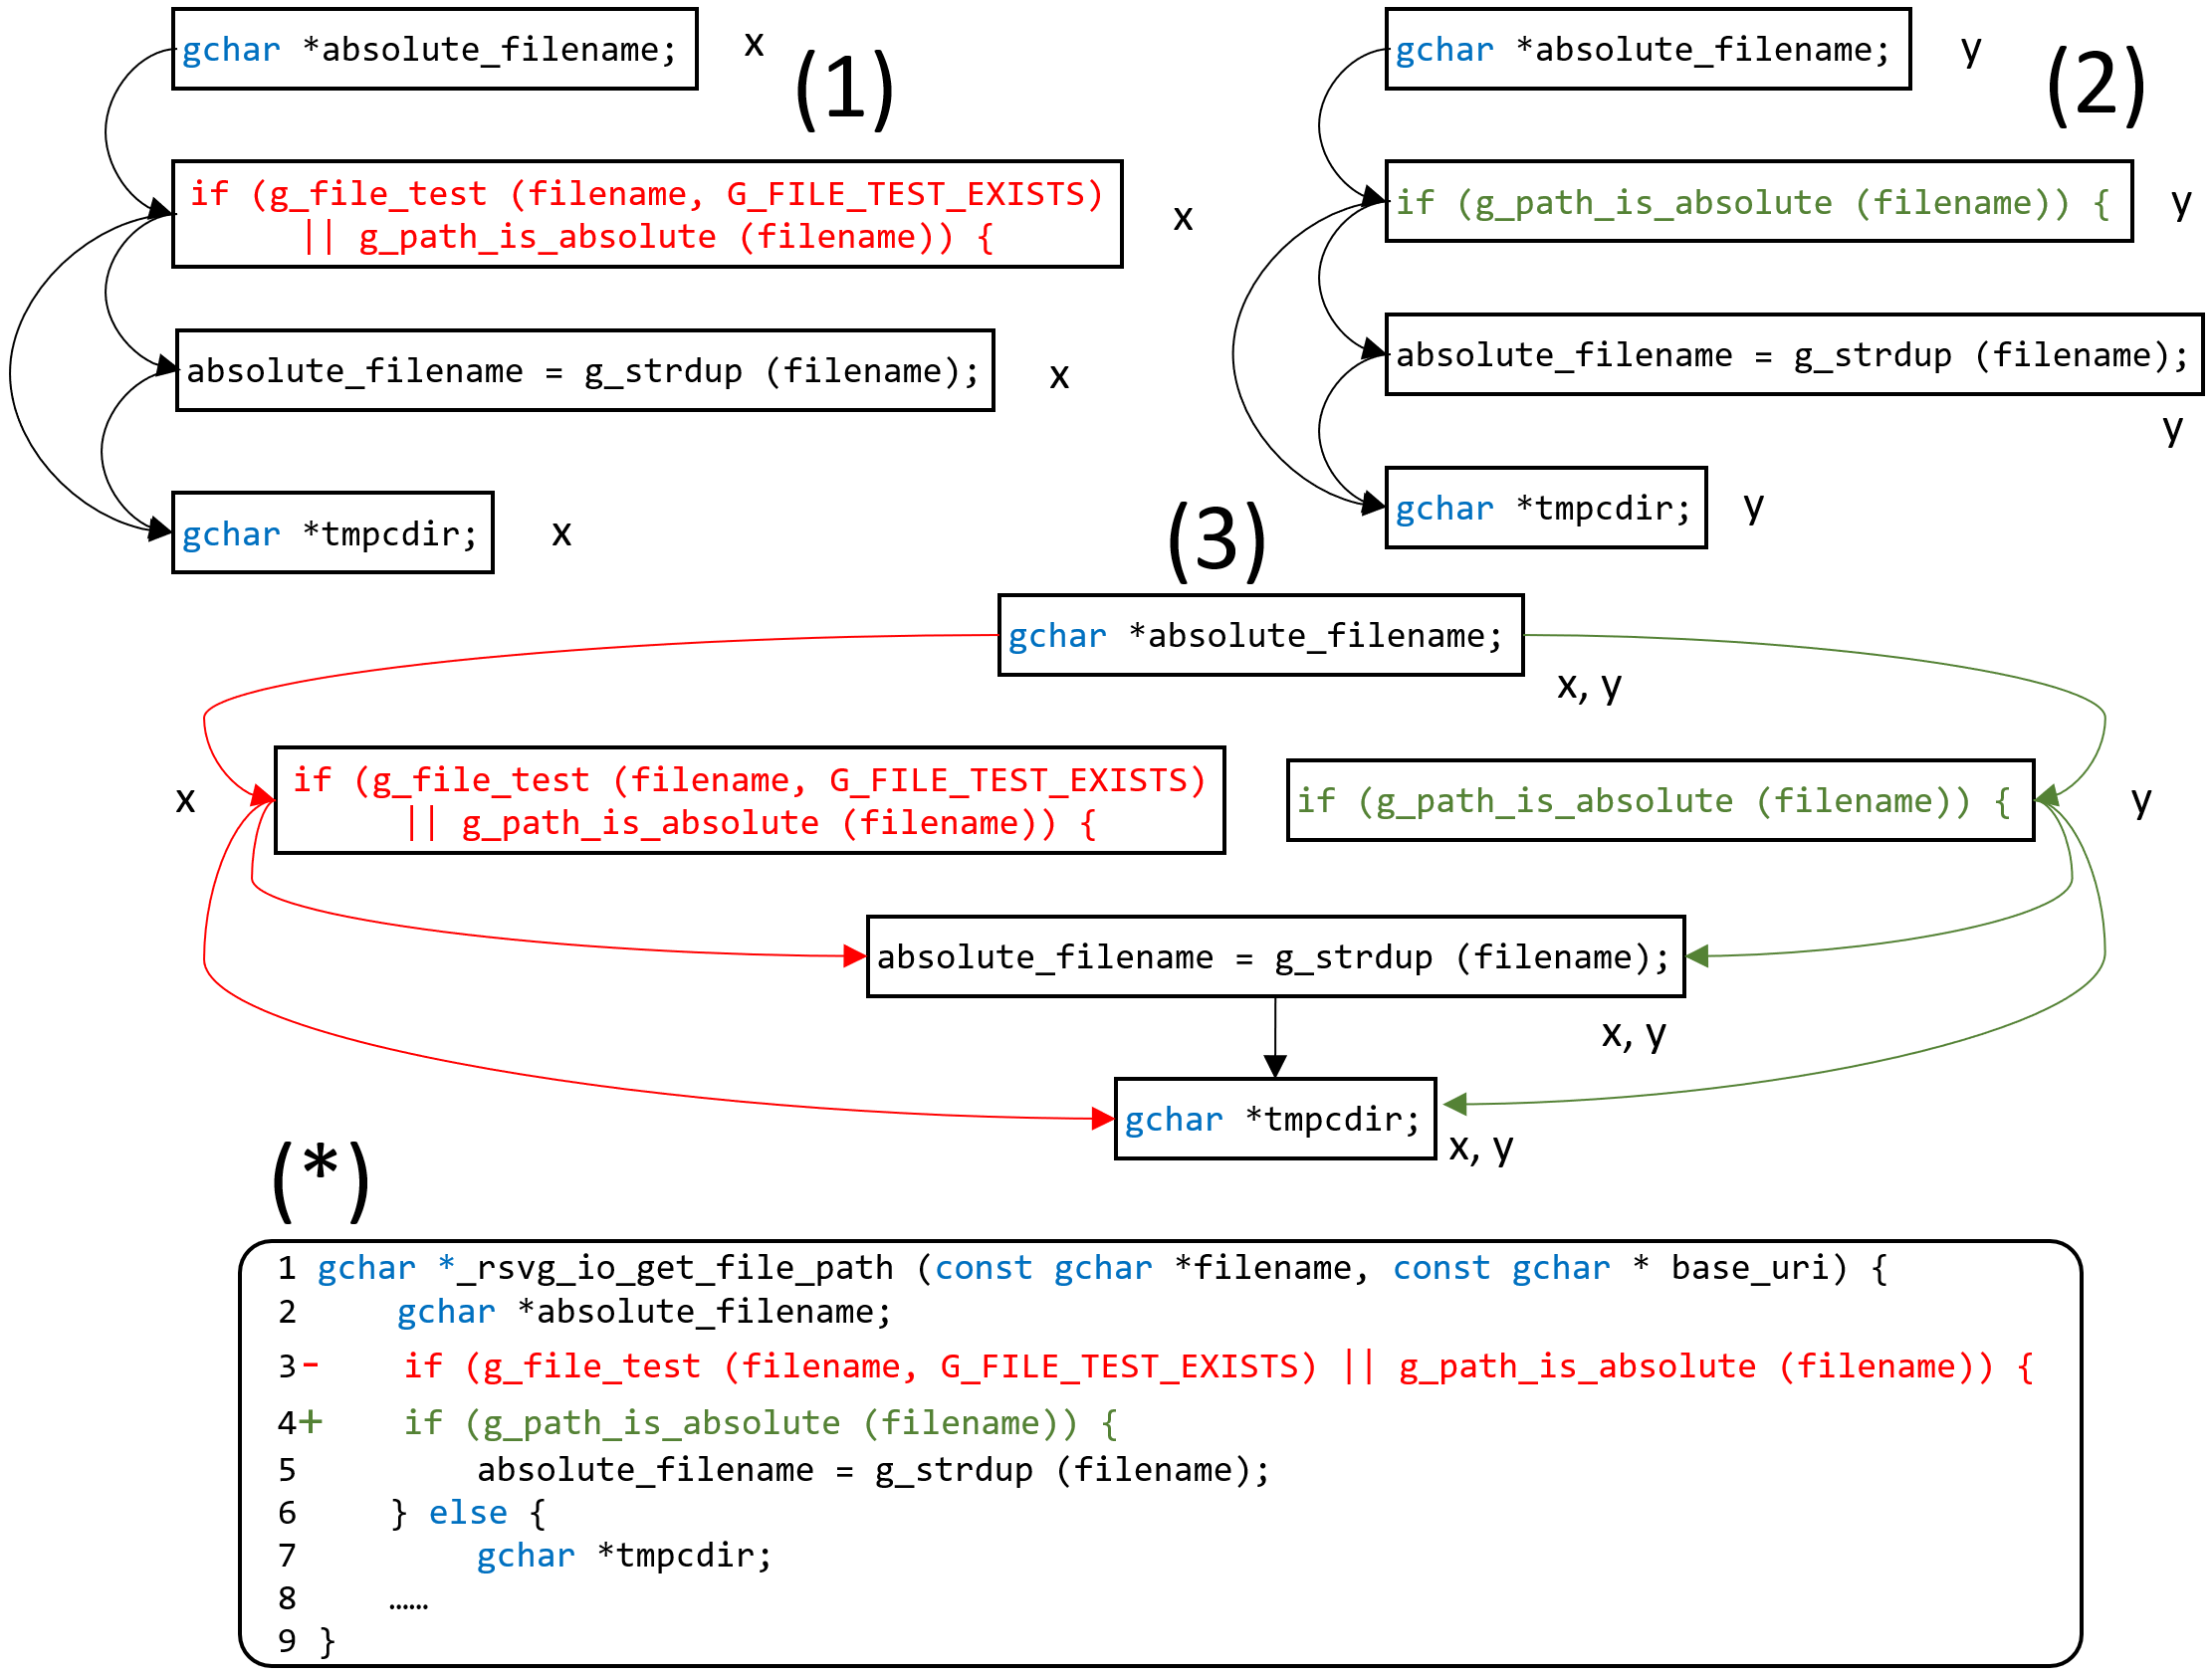
\includegraphics[width=3.2in]{graphs/multi-version-pdg.png}
	\vspace{-8pt}
	\caption{Multi-Version Program Dependence Graph}
        \vspace{-12pt}
	\label{fig:multi-version-pdg}
\end{figure}

%Let us next explain {\tool} in details.
The first step is to build the multi-version PDG.
%({\mvpdgxy}).
Figure~\ref{fig:multi-version-pdg}(*) shows the vulnerable method
\code{rsvg\_io\_get\_file\_path}. The change at line 3 into line 4 was
deemed as a vulnerability-introducing change by a detection tool, in
which \code{g\_file\_test(filename,} \code{G\_FILE\_TEST\_EXISTS)} was
removed from the condition at line
3. Figs~\ref{fig:multi-version-pdg}(1)
and~\ref{fig:multi-version-pdg}(2) display the PDGs of the method
\code{rsvg\_io\_get\_file\_path} before and after the change. All the
nodes of the PDG before the change are marked with $x$, and those of
the PDG after the change are marked with
$y$. Fig.~\ref{fig:multi-version-pdg}(3) shows the multi-version
PDG ({\mvpdgxy}) built from the two versions $x$ and
$y$ of that method before and after the change. In {\mvpdgxy}, the
nodes labeled with either $x$ or $y$ appear only in the PDG of the
version $x$ or $y$, respectively. The nodes labeled with ($x,y$)
appear in the PDGs at both versions.



%The first step of \tool is to use before and after versions of
%vulnerability bring in commits to build the {\mvpdgxy} graph. The
%{\mvpdgxy}\cite{flexeme-fse20} is a directed graph generated from the
%disjoint union of all nodes and edges in the version $x$ and the
%version $y$ of the programming dependency graph (PDG). For example,
%Figure~\ref{fig:multi-version-pdg} shows the code change in a
%vulnerability bringing commit in which part of the if condition
%\code{g\_file\_test(filename, G\_FILE\_TEST\_EXISTS)||} is
%removed. The top left and right figures in
%Figure~\ref{fig:multi-version-pdg} display the PDG of the method
%\code{rsvg\_io\_get\_file\_path} before (we call it version $x$) and
%after (we call it version $y$) the commit changes. The statements in
%the top left figure are marked as $x$ while the statements in the top
%right figure are marked as $y$. The big figure in the middle of the
%Figure~\ref{fig:multi-version-pdg} shows the {\mvpdgxy} in which the
%deleted/added statements are marked as $x$ or $y$ and the unchanged
%statements marked as $x, y$.

We adopt the multi-version graph building algorithm in
Flexeme~\cite{flexeme-fse20}. Specifically, we generate the PDGs
for both versions~$x$ and $y$. We run Git diff tool on the source
code to determine~the changed and unchanged nodes for the
statements. The added nodes are kept in $\delta$-PDG$^{x,y}$ with the
labels $y$ as they appear in the newer version $y$. We also retain the
deleted nodes and use the label $x$ for them. The unchanged nodes
between the versions are matched by using string similarity among the
respective statements to filter the candidates and line-span proximity
to rank them. When considering the edge changes, we back-propagate the
delete nodes to the edges flowing into them. We also add all unmatched
edges in the newer version $y$ to the PDG$^{x,y}$ as the edges
relevant to the added nodes.

%Details on building $\delta$-PDG$^{x,y}$ can be found in~\cite{flexeme-fse20}.



After building $\delta$-PDG$^{x,y}$, for each changed node in the
graph, \tool collects all the unchanged nodes within the $k$-hops and
the inducing edges among them to build a sub-graph as the context for
the changed node. $\delta$-PDG$^{x,y}$ and the context for each
changed node are used as the input next. Building
$\delta$-PDG$^{x,y}$ and contexts is needed in both training and
predicting.

%To build the {\mvpdgxy}, we follow the procedure from Flexeme~\cite{flexeme-fse20}. Specifically, we first generate the PDGs for both versions $x$ and $y$ of the source code. Secondly, we use the code diff tool to determine the changed (Including addition and deletion. The modified statement is regarded as one addition plus one deletion.) and unchanged statements between version $x$ and $y$. Thirdly, as for the changed statements, if the statements are added, \tool mark them as $y$ because they appear in the later version $y$, and if the statements are deleted, \tool marks them as $x$. As for the unchanged statements, \tool matches them by using string similarity among the respective statements to filter the candidates and line-span proximity to rank them. Fourthly, to consider the edges between two versions, \tool back-propagates the delete nodes (statements) to the edges flowing into them. We also add all unmatched edges in the newer version $y$ to the {\mvpdgxy} as the edges relevant to the added nodes (statements). More details on building {\mvpdgxy} can be found in~\cite{flexeme-fse20}.


%\section{Graph-based Representation Learning for Contextualized Embeddings for Code Changes}

\section{Graph-based, Contextualized Embeddings for Code Changes}
\label{embedding:sec}

\begin{figure*}[t]
	\centering
	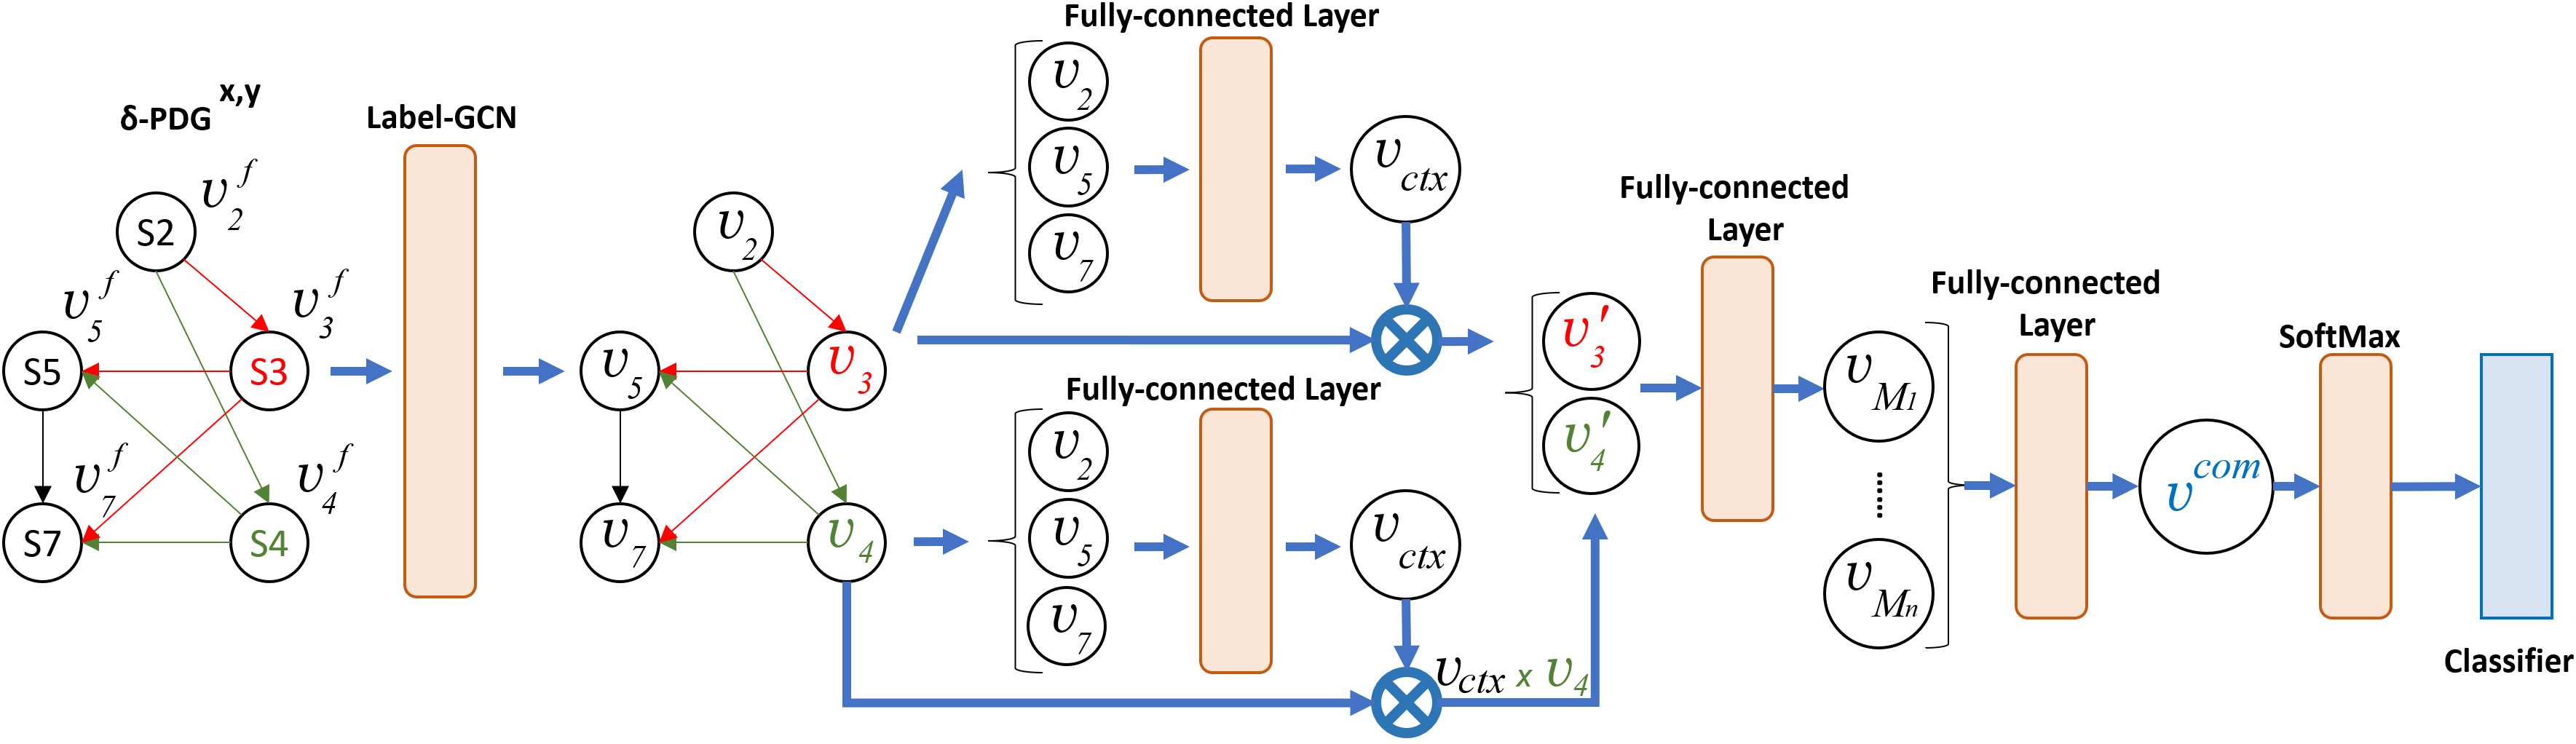
\includegraphics[width=5.8in]{graphs/model-4.png}
	\vspace{-10pt}
	\caption{Context-aware, Graph-based Representation Learning for Contextualized Embeddings for Code Changes}
	\label{fig:step-2}
\end{figure*}

The goal of our representation learning model is to build the {\em
  code change contextualized embeddings} that integrate both {\em
  program dependencies and contexts}.  From those embeddings, {\tool}
builds the embedding for the entire commit, which will be used in the
classification tasks for detection and assessment.

%After the previous step, we obtain the {\mvpdgxy} and the context
%sub-graphs for the changed nodes in {\mvpdgxy}.
%In this step, {\tool} aims to learn the vector/embedding to represent
%the code changes in a commit.
%The embeddings are used to train a model to learn the classifications
%of the commit for a specific vulnerability assessment type.

%with the code change context in the last step, in this step, the goal is to learn the representation vector for code changes in a commit and use the learned representation vector to do the classification for a specific vulnerability assessment type. The key point of the code change representation learning is {\em contextualized} which includes the influence of surrounding source code and the dependency relationships.

\subsection{Feature Vectors $v^{f}_n$ for {\mvpdgxy} Nodes}
\label{feature:sec}

After the previous step, we obtain {\mvpdgxy} and the context
sub-graphs for the changed nodes in {\mvpdgxy}. We leverage
Label-GCN~\cite{label-gcn} to model {\mvpdgxy} as follows. We first
build the node feature vector for each node $n$ in {\mvpdgxy}. To do
so, we use the sequence of the code tokens $t_n$ of the statement $s$
corresponding to $n$. We use a word embedding
model to learn the vector $v_t$ for each token when we consider the
code token sequence for $s$ as a sentence. The {\em node content
  vector} for $n$ is computed as the average vector $v_{avg}$ of
all the vectors $v_t$ of all the tokens in the statement $s$.
%We compute the average vector $v_{avg}$ of all the vectors $v_t$ of
%all the tokens in the statement $s$, and consider $v_{avg}$ as the
%{\em node content vector}.
%
To integrate the labels $x$, $y$, and ($x,y$) into the node feature,
we use a one-hot vector with the length of 3 for those labels. By
concatenating the node content vector with the one-hot vector for the
labels, we have the {\em node feature~vector $v^{f}_n$} for the node
$n$. 

%To obtain the vectors for the nodes in the $\delta$-PDG, we need: (a)
%statement node vector, (b) feature vector, (c) Label-GCN. Each
%statement node in the $\delta$-PDG is essentially a sequence of code
%tokens. We obtain its vector (a) by taking an average of the GloVe
%embeddings for all tokens in the code sequence. Next, we obtain the
%feature vector incorporating the label information in a node, i.e.,
%(b) which is a one-hot vector of the version labels
%(lines_537_549). Concatenating (a) and (b) gives the vectors for the
%nodes in the $\delta$-PDG that is fed into the Label-GCN, which
%through Equations (1)-(3), generate the vector/embedding for each node
%in $\delta$-PDG.


%No need for this para
%To achieve that, we first use the Label-GCN \cite{label-gcn} to model
%{\mvpdgxy}. The first advantage of using Label-GCN is its ability to
%capture the dependencies among the statements represented by the
%nodes. The second advantage comes from the ability to support and
%consider the labels during the computing the vectors of the nodes. We
%use the label mechanism in Label-GCN to represent the labels for the
%versions $x$ and $y$. Specifically, the label $x$ is for a deleted
%node, $y$ for an inserted node, and ($x,y$) for an un-changed node.

\subsection{Contextualized Embedding $v_n$ for Node $n$}
\label{label-gcn-compute}

Next, we replace each node $n$ in {\mvpdgxy} with the node feature
vector~$v^{f}_n$.
%and feed the graph to the Label-GCN to generate the embedding $v_n$
%for each node~$n$.
Similar to the traditional GCN~\cite{gcn}, Label-GCN~\cite{label-gcn}
takes the graph with the node feature vectors as the input and
generates the embeddings for each node in the graph. In addition, for
the current node, in the first layer, Label-GCN considers the change
labels of the neighboring nodes as part of the feature vectors.
%it accepts the node labels in the first layer to better integrate the
%features from the neighboring nodes based on the known labels. To
%consider the label information, it takes the labels of the neighboring
%nodes into account as parts of the features of neighboring
%nodes.
Label-GCN generates the representation vectors (embeddings) for the nodes in each
layer as follows:
\begin{equation}\label{eq1}
	H_{(l)} = 
	\begin{cases}
		\sigma [(\hat{A}X-diag(\hat{A})\sum_{j=1}^{K}e_je^T_j)W^0] &  l = 1\\
		\sigma (\hat{A}H^{(l-1)}W^{(l-1)}) &  l \geq 1\\
	\end{cases}
\end{equation}
\begin{equation}\label{eq2}
	\hat{A} = \tilde{D}^{-\frac{1}{2}}\tilde{A}\tilde{D}^{-\frac{1}{2}}
\end{equation}
\begin{equation}\label{eq3}
	\tilde{A} = A + I
\end{equation}
Where $H$ is the output for hidden layers; $A$ is the
adjacency~matrix and $I$ is the identity matrix; $\tilde{D}$ is the diagonal node degree matrix; $W$
is the weight matrix; $X$ is the input and $X \in R^{num \times (d+K)}$;
$num$ is the number of nodes;~$d$ is the dimension of node features;
$K$ is the number of types of node labels in the input ($K$=3 for $x$,
$y$, and ($x,y$)); and $-diag(\hat{A})\sum_{j=1}^{K}e_je^T_j$ is used
to eliminate the self-loops for the components of the feature vectors
for the labels.

The vectors $H(l)$ at the output layer are used as the vectors $v_i$s
for the nodes in the {\mvpdgxy} graph after Label-GCN in Figure~\ref{fig:step-2}.



%Those feature vectors and the connections among the nodes in
%{\mvpdgxy} will be fed into the Label-GCN model.

%To make the Label-GCN can work on the incoming {\mvpdgxy}, \tool firstly generates the node feature vector for each node $n$ in the {\mvpdgxy}. To do that, \tool regards the content of each node $n$ (the content is the statement) as a sequence of token $t_n$ and then uses the GloVe \cite{} to learn the embedding vector $v_t$ for each token. Then \tool uses the average vector $v_{avg}$ for all token embedding vectors $v_t$ in node $n$ as the node content vector. To combine the label information $x$, $y$, and $x, y$ for each node into the node feature, \tool uses a one-hot vector with a length of $3$ to represent the label. By concatenating the node content vector with the one-hot vector for the label, each node $n$ in {\mvpdgxy} will have the node feature vector $v_{n}^{fea}$. Next, we feed the {\mvpdgxy} with the node feature vector for each node $n$ together to the Label-GCN to generate the representation vector $v_n$ for all nodes in the graph.

\subsection{Integrating Context and Building the Vector for a Commit}
\label{class:sec}

For each changed node $n_c$ in {\mvpdgxy}, we build the sub-graph
containing all the un-changed nodes in the $k$-hop neighbors of $n_c$
and use that sub-graph as the context for $n_c$. We merge the vectors $v_i$s
in the context into a matrix. We then use a fully connected layer on
the matrix to build the {\em context vector $v_{ctx}$} for
the context.

To integrate the context into the embeddings, we compute the final
vector $v{'}_{n_{c}}$ for the changed node $n_c$ by performing the
cross-product between $v_{ctx}$ and the vector $v_{n_c}$ for $n_c$
computed by the Label-GCN model as described in
Section~\ref{label-gcn-compute}:$v{'}_{n_c} = v_{ctx} \times
v_{n_c}$.
To compute the vector for the entire commit, we collect all
the vectors $v{'}_{n_c}$s of the changed nodes $n_c$ in {\mvpdgxy}
into a matrix. We apply a fully connected layer to learn
the vector $v_{Mi}$ for a changed method $Mi$. The vectors for all changed
methods are passed through another fully connected layer to get the
vector $v^{com}$ for the commit. This vector is fed
into each SoftMax classifier for each task.

%To generate the representation vector for code changes in a commit, \tool first collects all representation vectors for the unchanged nodes in its $k$-hop neighbors for each changed node $n_c$ in graph {\mvpdgxy}. And then \tool uses a fully connected layer to learn the vector $v_{ctx}$ representing the context of the changed node $n_c$ by using the merged matrix that is built with all collected representation vectors as the input. Next, \tool calculates the final representation vector $v'_{n_c}$ by using the cross product to combine the representation vector $v_{n_c}$ for Label-GCN and $v_{ctx}$. After this, to consider on the whole commit level, \tool puts all representation vector $v'_{n_c}$ for the changed nodes $n_c$ in {\mvpdgxy} as a matrix, and then apply the other fully connected layer to learn the final vector $v^{com}$ for the entire commit. By having the commit-level representation vector $v^{com}$, \tool uses a SoftMax layer as the classifier to classify the commit for a specific type of vulnerability assessment. As for the details for all types of vulnerability assessment, we will introduce them in the next step.

\subsection{Illustrating Example}

Figure~\ref{fig:step-2} illustrates the vector building for the code
changes in Figure~\ref{fig:multi-version-pdg}. From
{\mvpdgxy}, we compute the node feature vectors $v^{f}_n$
(Section~\ref{feature:sec}) for all statement nodes $S_2$,...,$S_7$ in
that graph. Label-GCN takes that graph with node feature vectors to
generate the embeddings $v_2$,..., $v_7$ for the nodes
(Section~\ref{label-gcn-compute}).

%Figure \ref{fig:step-2} shows the procedure of contextualized embeddings for code changes step by using the case in Figure \ref{fig:multi-version-pdg} as an example. In the Figure, $S_2$, ..., $S_7$ are the statements in $Line-2$, ..., $Line-7$. The \tool uses Label-GCN takes the {\mvpdgxy} as input for Label-GCN model to generate the representation vectors for each node ($V_2$, ..., $V_7$).

Let us consider the changed nodes, $n_3$ and $n_4$. The context for
$n_3$ with one-hop distance includes $n_2$, $n_5$, and
$n_7$. Similarly, the context for $n_4$ includes the same nodes. After
merging those vectors into a matrix, which is passed through a
fully-connected layer, we obtain the context vectors $v_{ctx}$ for
$n_3$. Similarly, we obtain $v_{ctx}$ for $n_4$. Then, the final
contextualized vector for the changed node $n_3$ taking the context
into account is computed as the cross-product: $v'_3$ = $v_{ctx}$
$\times$ $v_3$. Similarly, $v'_4$ = $v_{ctx}$ $\times$ $v_4$.
%
We then put the vectors $v'_3$ and $v'_4$ together in a matrix and use
a fully-connected layer (FCL) to produce the method vector
$v_{M1}$.~All changed method vectors are passed through another FCL to
get $v^{com}$ for the commit. Finally, we pass $v^{com}$ to a SoftMax
layer to perform vulnerability detection or the classification for an
assessment type (e.g., {\em None}, {\em Partial}).

%Then for the changed nodes ($S_3$ and $S_4$), \tool collects the 1-hop neighbors for each of them including $V_2$, $V_5$, and $V_7$. By merging these vectors into a matrix and passing through the fully-connected layer, \tool gets the $V_{ctx}$ for $V_3$ and $V_4$ separately

%(The context for changed statements could be different. The 1-hop context for $V_3$ and $V_4$ are the same just a special case.). And then, by using the cross product to combine $V_{ctx}$ with $V_3$ and $V_{ctx}$ and $V_4$, we have $V'_3$ and $V'_4$.

%By putting them together as a matrix and passing it into the other fully-connected layer, \tool gets the representation vector $V^{com}$ for the entire commit. In the end, \tool passes the $V^{com}$ to a SoftMax layer to do the classification for the vulnerability assessment.


\section{Multi-Task Learning for Prediction and Assessment Classification}
\label{multi-task:sec}

In the previous sections, we have explained how {\tool} performs a
classification task for detection or assessment.
%the classification for vulnerability detection and for a
%vulnerability assessment type (VAT).
In this section, we will explain our multi-task learning mechanism to
perform the classification for vulnerability prediction (VD) and the
classifications for seven VATs with the following prediction
classes for each VAT:

\begin{enumerate}
	\item {\bf Confidentiality}: None; Partial; Complete
	\item {\bf Integrity}: None; Partial; Complete
	\item {\bf Availability}: None; Partial; Complete
	\item {\bf Access Vector}: Local; Network
	\item {\bf Access Complexity}: Low; Medium; High
	\item {\bf Authentication}: None; Single
	\item {\bf Severity}: Low; Medium; High
\end{enumerate}

%\item {\bf Severity}: Low (0.0-3.9); Medium (4.0-6.9); High (7.0-10.0)

%With the SoftMax layer, \tool is able to do the classification for different vulnerability assessment types. In \tool, we follow the existing study DeepCVA \cite{} to do the classification on seven vulnerability assessment types. For each of them, we follows the CVSS's definition on the national vulnerability database \cite{}. These vulnerability assessment types with the classes for each type are listed as follow:

As explained in Section~\ref{class:sec}, the vector $v^{com}$
representing the entire commit is passed through a SoftMax layer for
the classification for vulnerability detection or for a specific VAT.
%Let us call it a classification task.
In CAT, the multi-task learning mechanism uses the uncertainty
weighted multi-task loss~\cite{kendall2018multi} to learn all 
classification tasks at the same time. Specifically, for each
classification task, \tool uses a cross-entropy loss function to do
the classification as follows:
\begin{equation}\label{eq4}
	L = -log(Softmax(y, f(x)))
\end{equation}
Where $f(x)$ is the output of a classification task $f$; y is the
ground truth. To get the joint loss function for all the tasks with
uncertainty weighting, following Kendall {\em et
  al.}'s~\cite{kendall2018multi}, we have
\begin{equation}\label{eq5}
	L_i(W) = -log(Softmax(y_i, f^W(x_i)))
\end{equation}
\begin{equation}\label{eq6}
	L(W, \sigma_1, \sigma_2, ..., \sigma_7) = \sum_{i=1}^7\frac{1}{2\sigma_i^2}L_i(W) + log \sigma^2_i
\end{equation}
Where $W$ is the weight adding to the input, $\sigma_i$ is the
$i^{th}$ noise scalar, and $W$ and $\sigma_i$ are both trainable in
the model.

With Formula (\ref{eq6}), {\tool} uses the multi-task
learning to train all classification models together with the
features for each task. For training, we set as the objective the
highest average F-score or MCC (Section~\ref{method:sec}) for all
tasks. For prediction, the trained model produces the
classification results for VD and for all VATs.

%In brief, the multi-task learning can help propagate the mutual impact
%of the important features for each VAT classification task on the
%other tasks and vice versa, leading to the highest accuracy for all
%seven classification~tasks.





\section{Empirical Evaluation}

%We conducted several experiments to evaluate {\tool} against the
%state-of-the-art vulnerability assessment approach. All experiments
%were conducted on a server with 16 core CPU and a single Nvidia A100 GPU.

%We conducted several experiments to evaluate {\tool}. We aim to answer
%the following questions:

To evaluate {\tool}, we seek to answer the following questions:

%\subsection{Research Questions}
%To evaluate {\tool}, we answer the following questions:

%\vspace{3pt}

\vspace{1pt}
\noindent\textbf{RQ1. Comparison with State-of-the Art ML-based Vulnerability
Detection Approaches on C dataset.} How well does {\tool} perform
compared with the existing DL-based VD approaches?

\vspace{1pt}
\noindent\textbf{RQ2. Comparison in Vulnerability Assessment on C
  Dataset.} How well does {\tool} perform compared to the
state-of-the-art model in vulnerability assessment on a C dataset?

  %Vulnerability Assessment Comparative Study on Java Dataset.} How well does {\tool} perform in comparison with
%the state-of-the-art approaches for assessing vulnerabilities in Java?

\noindent\textbf{RQ3. Contextualized Embeddings for Code Changes.} Do {\tool}'s embeddings help it improve over the
baseline in classifications?

%What are the characteristics of code change embeddings in VA?

\noindent {\bf RQ4. Explainable AI to Study Relevant Features on Program Dependencies.} Does {\tool} use program dependencies in vulnerability detection and assessment?

In RQ3 and RQ4, we aim to evaluate the extent of contributions of two
  {\tool}'s key design choices, i.e., {\em contextualized embeddings
  for code changes} and~{\em program dependencies} to its performance.

%\vspace{3pt}
%\noindent\textbf{RQ5. Overlapping Analysis.} How many vulnerabilities
%are assessed correctly by a model and not by another one?

%\vspace{3pt}
\noindent\textbf{RQ5. Ablation Study on Multi-Task Learning and Context.} How do multi-task
learning and context affect {\tool}'s performance in vulnerability
detection and assessment?

\vspace{1pt}
\noindent\textbf{RQ6. Comparison in Vulnerability Assessment on Java
  Dataset.} How does {\tool} perform compared to the
state-of-the-art model in vulnerability assessment on a Java dataset?

\subsubsection{\textbf{Datasets}}\label{dataset}
%\begin{table}[h]
%	\caption{Statistics on Dataset}
%	\vspace{-15pt}
%	\begin{center}
%		\renewcommand{\arraystretch}{1}
%		\begin{tabular}{p{1.6cm}<{\centering}p{3cm}<{\centering}p{1cm}<{\centering}p{1.5cm}<{\centering}p{2cm}<{\centering}}
%		\end{tabular}
%		\label{DataSet}
%	\end{center}
%	\vspace{-10pt}
%\end{table}

We used two vulnerability datasets in C and Java: BigVul
2.0~\cite{bigvul-msr20} and CVAD~\cite{deepCVA-ase21}
(Table~\ref{dataset:tab}).
%Both were built by crawling the Common Vulnerabili\-ties and Exposures
%(CVE) database and the code repositories mentioned in the CVEs.
Both were manually~checked and used in prior
research~\cite{bigvul-msr20,li2021vulnerability,deepCVA-ase21}. Experiments were
conducted on a server with 16 core CPU and a single Nvidia A100 GPU.

%Table~\ref{dataset:tab} shows the statistics of the datasets.

%In this paper, we evaluate approaches on vulnerabilities in C and Java using two different datasets: BigVul~2.0~\cite{} and DeepCVA-dataset~\cite{} (CVAD).  Both BigVul2.0 and DeepCVA-dataset are built by crawling the public Common Vulnerabilities and Exposures database~\cite{} and CVE-related source code repositories. BigVul~2.0 is in C and DeepCVA-dataset is in Java. Table~\ref{} shows the statistics of two datasets.


\begin{table}[t]
	\caption{Statistics of BigVul and CVAD Datasets}
        \tabcolsep 2.5pt
        \vspace{-10pt}
	\begin{center}
%        \footnotesize
\small
		\renewcommand{\arraystretch}{1}
		\begin{tabular}{l|p{1.5cm}<{\centering}|p{2cm}<{\centering}}
			
        	Datasets	& BigVul (C) & CVAD (Java)\\\hline
		\# of Projects  & 303 & 246 \\\hline
	    \# of Vulnerabilities & 3336 & 542\\\hline
     	\# of Vulnerability Introducing Commits & 7851 & 1229\\\hline

		\end{tabular}
		\label{dataset:tab}
	\end{center}
%	\vspace{-10pt}
\end{table}







\subsection{Experimental Methodology}
\label{method:sec}

\subsubsection{\textbf{Datasets}}\label{dataset}
%\begin{table}[h]
%	\caption{Statistics on Dataset}
%	\vspace{-15pt}
%	\begin{center}
%		\renewcommand{\arraystretch}{1}
%		\begin{tabular}{p{1.6cm}<{\centering}p{3cm}<{\centering}p{1cm}<{\centering}p{1.5cm}<{\centering}p{2cm}<{\centering}}
%		\end{tabular}
%		\label{DataSet}
%	\end{center}
%	\vspace{-10pt}
%\end{table}

We used two vulnerability datasets in C and Java: BigVul
2.0~\cite{bigvul-msr20} and CVAD~\cite{deepCVA-ase21}
(Table~\ref{dataset:tab}).
%Both were built by crawling the Common Vulnerabili\-ties and Exposures
%(CVE) database and the code repositories mentioned in the CVEs.
Both were manually~checked and used in prior
research~\cite{bigvul-msr20,li2021vulnerability,deepCVA-ase21}. Experiments were
conducted on a server with 16 core CPU and a single Nvidia A100 GPU.

%Table~\ref{dataset:tab} shows the statistics of the datasets.

%In this paper, we evaluate approaches on vulnerabilities in C and Java using two different datasets: BigVul~2.0~\cite{} and DeepCVA-dataset~\cite{} (CVAD).  Both BigVul2.0 and DeepCVA-dataset are built by crawling the public Common Vulnerabilities and Exposures database~\cite{} and CVE-related source code repositories. BigVul~2.0 is in C and DeepCVA-dataset is in Java. Table~\ref{} shows the statistics of two datasets.


\begin{table}[t]
	\caption{Statistics of BigVul and CVAD Datasets}
        \tabcolsep 2.5pt
        \vspace{-10pt}
	\begin{center}
%        \footnotesize
\small
		\renewcommand{\arraystretch}{1}
		\begin{tabular}{l|p{1.5cm}<{\centering}|p{2cm}<{\centering}}
			
        	Datasets	& BigVul (C) & CVAD (Java)\\\hline
		\# of Projects  & 303 & 246 \\\hline
	    \# of Vulnerabilities & 3336 & 542\\\hline
     	\# of Vulnerability Introducing Commits & 7851 & 1229\\\hline

		\end{tabular}
		\label{dataset:tab}
	\end{center}
%	\vspace{-10pt}
\end{table}







%To evaluate the performance of automated commit-level vulnerability assessment, we use the following two metrics: F1-Score and Matthews Correlation Coefficient (MCC). These two metrics have been widely, commonly, and frequently in the literature (check deepcva page 6, evaluation metrics for literature). Due to the fact that our {\tool} is built for multi-class classification, we used the macro F1-Score and multi-class version of MCC as in~\cite{le2021deepcva}.


\subsubsection{\textbf{Analysis Approaches for RQs\\}}

\noindent\textbf{RQ1. Comparison on Vulnerability Detection on C dataset}

\emph{Baselines}. We include {\bf VCCFinder}~\cite{perl2015vccfinder}
(a commit-level ML-based VD), and other ML VD tools:
\textbf{VulDeePecker} \cite{li2018vuldeepecker}, \textbf{Devign}
\cite{zhou2019devign}, \textbf{SySeVR} \cite{li2021sysevr},
\textbf{Russell} {\em et al.}  \cite{russell2018automated},
\textbf{Reveal} \cite{chakraborty2021deep}, and {\bf IVDetect}
\cite{li2021vulnerability}. Except VCCFinder, we ran the others
on the code after commit. 

\emph{Procedure.}  We use all vulnerable methods and randomly select
the same number of non-vulnerable methods from the fixed version
projects, to build a dataset with the vul:non-vul ratio of 1:1. We
also evaluate the tools with the real-world ratio of 9:1. We randomly split the
data 80\%, 10\%, 10\% on the project basis without changing the
vul:non-vul ratio for training, tuning, and testing.

\emph{Parameter Tuning.}  For {\tool}, we used
autoML~\cite{NNI} for tuning the following hyper-parameters to have the
best performance: (1) Epoch size (100, 200, 300); (2) Batch size (64,
128, 256); (3) Learning rate (0.001, 0.003, 0.005, 0.010); (4) word embeddings length (150, 200, 250, 300). We
tuned DeepCVA's parameters from its documentation.
%We use AutoML~\cite{NNI} on all models to automatically tune
%hyper-parameters on the tuning dataset. We tuned \tool with the
%parameters \textit{batch size, hidden size, learning rate, dropout
%  rate}. The hyper-parameters we tuned for the baselines can be found
%in their papers. We choose the hyper-parameters with the best accuracy
%for each model.

\emph{Evaluation Metrics.} We use the following metrics to measure the
effectiveness of a model: $Recall = \frac{TP}{TP+FN}$, $Precision =
\frac{TP}{TP+FP}$, and $F\-score =
\frac{2*Recall*Precision}{Recall+Precision}$.
%\begin{equation}
%	Recall = \frac{TP}{TP+FN}
%\end{equation}
%\begin{equation}
%	Precision = \frac{TP}{TP+FP}
%\end{equation}
%\begin{equation}
%	F\_score = \frac{2*Recall*Precision}{Recall+Precision}
%\end{equation}
where TP = True Positives; FP = False Positives; FN = False Negatives; TN = True Negatives.

%Recall measures how many of the vulnerable methods can be correctly detected, while Precision is used to measure how many of the detected vulnerable methods are indeed labeled as vulnerable in the collected dataset. F-score is used to reflect the overall performance by combining both the Recall and Precision.

%\vspace{3pt}
\noindent\textbf{RQ2. Comparison on Vulnerability Assessment on C dataset.}

{\em Baseline and Procedure.} We compare {\tool} with
DeepCVA~\cite{deepCVA-ase21}. We ran the models on BigVul. We used the
same longitudinal setting in~\cite{deepCVA-ase21,falessi2020need} for
training, validation, and testing to mimic the real-world scenario in
which the older vulnerabilities are used for training to assess the
newer. Specifically, we sorted all the commits in a chronological
order based on their absolute time. We divided the commits into 10
equal folds from oldest to newest. For a fold $k$ ($k$ $\le$ $8$), we used
all the folds 1 to $k$ for training, the $(k$+$1)^{th}$ and $(k$+$2)^{th}$
folds for validation and testing. Models are tuned as in~RQ1.

%\subsubsection{\textbf{Evaluation Metrics}}

%To evaluate the models' performance in automated vulnerability
%assessment,

\emph{Evaluation Metrics.} We use the same metrics in
DeepCVA~\cite{deepCVA-ase21}: F-score and Matthews Correlation
Coefficient (MCC). F-score ranges from 0 to 1 (the best), and MCC
ranges from -1 to 1 (the best). F-score is a metric to evaluate
classification tasks. We chose F-score to handle the class imbalance
prevalent in some of the VATs. Because we evaluate the classification
models with multiple classes, we used the macro
F-Score~\cite{spanos2018multi} and the multi-class version of
MCC~\cite{gorodkin04}. The overall MCC is computed as the average of
the MCCs for all classification tasks as in DeepCVA~\cite{deepCVA-ase21}.

%We turned {\tool} with the following key hyper-parameters ....
%We turned DeepCVA with the following key hyper-parameters ...
%We use macro F1-Score and multi-class MCC to evaluate both approaches.


%We also tuned the models as in RQ1.

%In this RQ, we compare {\tool} with the same baseline in RQ1, DeepCVA. We ran {\tool} and DeepCVA on the Java dataset, DeepCVA-dataset~\cite{} (CVAD).  We used the same time-series data splitting strategy as the one in RQ1 to train, validate, and test both models.


%we randomly split the BigVul into xx\% for training, xx\% for validation, and xx\% for testing.


%We turned {\tool} with the following key hyper-parameters .... As we reused the dataset from the DeepCVA, we directly tune DeepCVA with the parameters reported in their paper. Same as RQ1, we use macro F1-Score and multi-class MCC to evaluate both approaches.

%\vspace{1pt}
\noindent\textbf{RQ3. Code Change Embedding Analysis.} We evaluate the impact of the embeddings in the classification for VATs.

\noindent \textbf{RQ4. Program Dependencies.} We use
Explainable AI to show that {\tool} in fact leverages program
dependencies in VDA.

%\vspace{1pt}
%\noindent\textbf{RQ5. Overlapping Analysis.}  We counted the
%vulnerabilities that were correctly assessed by {\tool} but
%not by DeepCVA and vice versa, and the ones
%that were correctly classified by both.


\vspace{1pt}
\noindent\textbf{RQ5. Ablation Study on Multi-Task Learning and
  Context.}  We evaluate the impacts of key factors in {\tool}: (1)
multi-task learning, and (2) change context. We conducted ablation analysis
by removing a main factor from the model and made a comparison.
%d it with the xcomplete model.

\vspace{3pt}
\noindent\textbf{RQ6. Comparison on Assessment on CVAD (Java dataset).}

{\em Baseline and Procedure.} We compared {\tool} with the baseline
DeepCVA~\cite{deepCVA-ase21}. We used the same procedure, tuning, and
longitudinal setting as in RQ1, but on the Java~dataset.

%For (3), we used GNNExplainer~\cite{GNNExplainer} (Section~\ref{discuss:sec}).



%We aim to show the insights that {\tool}'s embeddings for code changes
%help improve automated vulnerability assessment over
%DeepCVA~\cite{deepCVA-ase21}.



%We aim to study the projections of the code changes in the commits
%with respect to different vulnerability assessment types.


%\vspace{-0.05in}
\section{Experimental Results}

\subsubsection{{\bf Comparison on Vulnerability Detection on C Dataset (RQ1)}}
\label{sec:vd-result}

\begin{table} [t]
  \caption{Vulnerability Detection on C Dataset (RQ1)}
  \vspace{-5pt}
  \begin{center}
    \small
			\begin{tabular}{cccc}
				\toprule
\textbf{Approach} & \textbf{Precision} & \textbf{Recall} & \textbf{F-score}  \\
\midrule
VulDeePecker~\cite{li2018vuldeepecker}      & 0.55             & 0.77          & 0.64           \\
SySeVR~\cite{li2021sysevr}            & 0.54             & 0.74           & 0.63           \\
Russell \textit{et al.}~\cite{russell2018automated} & 0.54       & 0.72          & 0.62            \\
Devign~\cite{zhou2019devign}           & 0.56             & 0.73          & 0.63           \\
Reveal~\cite{chakraborty2021deep}            & 0.62             & 0.69          & 0.65      \\
IVDetect~\cite{li2021vulnerability} & 0.54              & 0.77    & 0.67           \\
\midrule
{\tool}            & {\bf 0.72} & {\bf 0.90} & {\bf 0.81}\\
                \bottomrule
			\end{tabular}
			\label{tab:rq1}
                        \vspace{-12pt}
		\end{center}
\end{table}

%DeepVD            & \textbf{\begin{tabular}[c]{@{}c@{}}0.6997\\ (↑12.53\%)\end{tabular}}
%                  & \textbf{\begin{tabular}[c]{@{}c@{}}0.8827\\ (↑0.32\%)\end{tabular}}
%                  & \textbf{\begin{tabular}[c]{@{}c@{}}0.7806\\ (↑19.54\%)\end{tabular}} \\

As seen in Table~\ref{tab:rq1}, to detect vulnerability, {\tool}
improves over all the baselines in all the metrics. Specifically,
{\tool} relatively improves over the baseline models from {\bf 13.1\%--
  29.8\%} in Precision, from {\bf 15.8\%--29.2\%} in Recall, and from
{\bf 16.5\%--25.9\%} in F-score.


%To understand how {\tool} is complementary to the baselines, we
%compute how the top-100 result from {\tool} overlap with that from the
%top-performing baseline, IVDetect~\cite{fse21}. As seen in
%Figure~\ref{RQ1-overlap}, {\tool} can detect {\bf 19} vulnerable
%methods that IVDetect missed, while IVDetect can detect only {\bf 10}
%that {\tool} missed. Both detected the same 25 vulnerabilities. This
%result shows that {\tool} not only detects more vulnerabilities than
%the baselines, but also complements them.

%\begin{figure}[t]
%	\centering
%	\includegraphics[width=1.3in]{overlap.png}
%        \vspace{-5pt}
%	\caption{Overlapping Results between {\tool} and IVDetect}
%	\label{RQ1-overlap}
%\end{figure}

%-----------------------------------------------------------------

%\begin{figure}[t]
%	\centering
%	\lstset{
%		numbers=left,
%		numberstyle= \tiny,
%		keywordstyle= \color{blue!70},
%		commentstyle= \color{red!50!green!50!blue!50},
%		frame=shadowbox,
%		rulesepcolor= \color{red!20!green!20!blue!20} ,
%		xleftmargin=1.5em,xrightmargin=0em, aboveskip=1em,
%		framexleftmargin=1.5em,
%               numbersep= 5pt,
%		language=C++,
%    basicstyle=\scriptsize\ttfamily,
%    numberstyle=\scriptsize\ttfamily,
%    emphstyle=\bfseries,
%    moredelim=**[is][\color{red}]{@}{@},
%	escapeinside= {(*@}{@*)}
%	}
%\begin{lstlisting}[]
%BIO *PKCS7_dataDecode(PKCS7 *p7, EVP_PKEY *pkey, BIO *in_bio, X509 *pcert) {
%  ...
%  if (evp_cipher != NULL) {
%    ...
%    if (pcert == NULL) {
%      for (i = 0; i < sk_PKCS7_RECIP_INFO_num(rsk); i++) {
%        ri = sk_PKCS7_RECIP_INFO_value(rsk, i);
%        (*@{\color{red}{if (pkcs7\_decrypt\_rinfo(\&ek, \&eklen, ri, pkey) < 0)}}@*)
%           goto err;
%        ERR_clear_error();
%      }
%   } else {...}
%}
%\end{lstlisting}
%        \vspace{-12pt}
%        \caption{CVE-2019-1563: A vulnerable code in OpenSSL with 186 lines of code (after removed comments and empty lines). ReVeal and IVDetect failed to detect this but \tool did.}
%        \label{fig:rq1_example}
%\end{figure}


%PDT    & 145 & 144  \\
%EFG    & 145 & 295  \\
%PDG    & 145 & 477  \\
%CPG    & 622 & 1393 \\

Examining the results, we found that {\tool} often performed better
than the best baselines, Reveal~\cite{chakraborty2021deep} and
IVDetect~\cite{li2021vulnerability}, in the cases that the code
changes are relevant to the vulnerability. For example, a statement
(e.g., null check) was removed, leading to the vulnerable code (e.g.,
Null-Pointer Exception). Because examining both versions, {\tool} was
can detect better those vulnerability-introducing changes. The baselines
work only on the new version.

In Section~\ref{sec:ai}, we used {\em Explainable AI to display the
changed statements} in the code that contributes to the detected
vulnerability (Figure~\ref{gnn-example}). This is another advantage
from commit-level VD (pointing to the {\em fine-grained}
vulnerability-introducing change) that the VD tool working on the new
version only do not have.


%in the code with complex PDGs (which IVDetect uses as a key feature
%for detection) and CPGs (which Reveal uses for detection). Moreover,
%{\tool} detects vulnerabilities well with its code change embeddings.

%improper exception/error-handling.

%Fig.~\ref{fig:rq1_example} shows the vulnerable code from OpenSSL that
%was reported in CVE-2019-1563. The code (186 lines of code) has the
%PDG with 145 nodes and 477 edges, and the CPG with 622 nodes and 1,393
%edges. In contrast, PDT+EFG has 145 nodes and 295 edges (including the
%error-handling flows from line 8 to lines 9 and 10). Thus, complex PDG
%or CPG produce much noise for IVDetect and Reveal, which missed this
%vulnerability. {\tool} with its PDT+EFG features detects~well this
%type of vulnerability with improper error-handling (e.g., the
%incorrect code at line 8, which was fixed with an additional
%condition).

%=======================================

We also use a real-world vulnerability setting with a 9:1
non-vulnerability to vulnerability ratio. We randomly selected 10\% of
the vulnerable instances in the test set ten times, and finally took
the average of the performance. We report that the F-scores for
{\tool} and the top baseline IVDetect are 45.3\% and 25.4\%,
respectively. {\tool} exhibits a consistent trend with IVDetect while
outperforming it by 78.1\%. F-score is lower than in Table~\ref{tab:rq1} due to
unbalanced data.

%We report that F-score for {\tool} and the top baseline IVDetect are
%(45.3\%, 23.3\%) and (25.4\%, 20.4\%) respectively. {\tool} exhibits
%consistent trends with IVDetect while outperforming it by 78.1\% and
%14\% in Accuracy and F-score.

%\subsubsection{\bf Comparison on Vulnerability Assessment on C Dataset (RQ2)}




\begin{table}[t]
	\caption{Vulnerability Assessment on C Dataset (RQ2)}
        \vspace{-9pt}
	\begin{center}
%		\footnotesize
                \small
		\renewcommand{\arraystretch}{1}
		\begin{tabular}{l|p{1.9cm}<{\centering}|p{1.5cm}<{\centering}|p{1.5cm}<{\centering}}
			\hline
			\multirow{2}{*}{CVSS Metric}     & \multirow{2}{*}{Evaluation Metric}  & \multicolumn{2}{c}{Model}\\
			\cline{3-4}
		                                     &                                     & DeepCVA~\cite{deepCVA-ase21}    & {\tool}       \\
		    \hline
			\multirow{2}{*}{Confidentiality} & macro F1-score                             &     0.50       & 0.65\\
			\cline{2-4}
			                                 & MCC                                 &      0.23      & 0.31\\
			\hline
			\multirow{2}{*}{Integrity}       & macro F1-score                             &    0.42        & 0.55\\
			\cline{2-4}
			                                 & MCC                                 &    0.24        & 0.33\\
			\hline
			\multirow{2}{*}{Availability}    & macro F1-score                             &   0.47         & 0.63\\
			\cline{2-4}
			                                 & MCC                                 &    0.28        & 0.34\\
			\hline
			\multirow{2}{*}{Access Vector}   & macro F1-score                             &   0.58         & 0.69\\
			\cline{2-4}
			                                 & MCC                                 &    0.22        & 0.31\\
			\hline
			\multirow{2}{*}{Access Complexity} & macro F1-score                           &   0.49         & 0.66\\
			\cline{2-4}
			                                 & MCC                                 &    0.26        & 0.35\\
			\hline
			\multirow{2}{*}{Authentication}  & macro F1-score                             &   0.67         & 0.72\\
			\cline{2-4}
			                                 & MCC                                 &   0.36         & 0.39\\
			\hline
			\multirow{2}{*}{Severity}        & macro F1-score                             &   0.44         & 0.58\\
			\cline{2-4}
			                                 & MCC                                 &   0.23         & 0.28\\
			\hline
			\hline
			\multirow{2}{*}{Average}         & macro F1-score                             &    0.51        & 0.64 ($\Uparrow${\bf 25.5\%})\\
			\cline{2-4}
			                                 & MCC                                 & 0.26           & 0.33 ($\Uparrow${\bf 26.9\%})\\
            \hline
		\end{tabular}
		\label{rq1_results}
	\end{center}
\end{table}

In Table~\ref{rq1_results}, {\tool} relatively improves
DeepCVA~\cite{deepCVA-ase21} by {\em 25.5\% in macro F1-score and
26.9\% in multi-class MCC} on the overall multi-class VA
classification in C dataset. For specific VATs, {\tool} improves
DeepCVA by {\em 7.5--34.7\% in macro-F1-score and 8.3--40.9\% in
multi-class MCC}. Moreover, the largest relative improvement in macro
F1-score happens for {\em Access Complexity} and the largest relative
improvement in multi-class MCC happens for {\em Access Vector}. The
lowest relative improvement in both macro F1-score and multi-class MCC
happens for type {\em Authentication}, however, the absolute macro
F1-score (0.72) for {\em Authentication} is highest among all the
VATs.



%Table~\ref{rq1_results} shows that {\tool} outperforms the state-of-the-art baseline, DeepCVA, in the automation of commit-level vulnerability assessment on the C dataset. Particularly, {\tool} improves the state-of-the-art baseline by 25.5\% in terms of macro-F1-score, and 26.9\% in terms of multi-class MCC on the overall performance. The higher values of macro-F1-score and MCC indicate that {\tool} can perform more accurate multi-classification on C commits than DeepCVA. As for specific types of vulnerability assessment, {\tool} improves the state-of-the-art baseline by 7.5-34.7\% in terms of macro-F1-score and 8.3-40.9\% in terms of macro-F1-score. The lowest relative improvement of both macro-F1-score and multi-class MCC happens when testing the $Authentication$. At the same time, the biggest relative improvement of macro-F1-score happens when testing $Access Complexity$ and the biggest relative improvement of multi-class MCC happens when testing $Access Vector$.
























\subsubsection{\bf Comparison on Vulnerability Assessment on C Dataset (RQ2)}




\begin{table}[t]
	\caption{Vulnerability Assessment on C Dataset (RQ2)}
        \vspace{-9pt}
	\begin{center}
%		\footnotesize
                \small
		\renewcommand{\arraystretch}{1}
		\begin{tabular}{l|p{1.9cm}<{\centering}|p{1.5cm}<{\centering}|p{1.5cm}<{\centering}}
			\hline
			\multirow{2}{*}{CVSS Metric}     & \multirow{2}{*}{Evaluation Metric}  & \multicolumn{2}{c}{Model}\\
			\cline{3-4}
		                                     &                                     & DeepCVA~\cite{deepCVA-ase21}    & {\tool}       \\
		    \hline
			\multirow{2}{*}{Confidentiality} & macro F1-score                             &     0.50       & 0.65\\
			\cline{2-4}
			                                 & MCC                                 &      0.23      & 0.31\\
			\hline
			\multirow{2}{*}{Integrity}       & macro F1-score                             &    0.42        & 0.55\\
			\cline{2-4}
			                                 & MCC                                 &    0.24        & 0.33\\
			\hline
			\multirow{2}{*}{Availability}    & macro F1-score                             &   0.47         & 0.63\\
			\cline{2-4}
			                                 & MCC                                 &    0.28        & 0.34\\
			\hline
			\multirow{2}{*}{Access Vector}   & macro F1-score                             &   0.58         & 0.69\\
			\cline{2-4}
			                                 & MCC                                 &    0.22        & 0.31\\
			\hline
			\multirow{2}{*}{Access Complexity} & macro F1-score                           &   0.49         & 0.66\\
			\cline{2-4}
			                                 & MCC                                 &    0.26        & 0.35\\
			\hline
			\multirow{2}{*}{Authentication}  & macro F1-score                             &   0.67         & 0.72\\
			\cline{2-4}
			                                 & MCC                                 &   0.36         & 0.39\\
			\hline
			\multirow{2}{*}{Severity}        & macro F1-score                             &   0.44         & 0.58\\
			\cline{2-4}
			                                 & MCC                                 &   0.23         & 0.28\\
			\hline
			\hline
			\multirow{2}{*}{Average}         & macro F1-score                             &    0.51        & 0.64 ($\Uparrow${\bf 25.5\%})\\
			\cline{2-4}
			                                 & MCC                                 & 0.20           & 0.33 ($\Uparrow${\bf 26.9\%})\\
            \hline
		\end{tabular}
		\label{rq1_results}
	\end{center}
\end{table}

In Table~\ref{rq1_results}, {\tool} relatively improves over DeepCVA~\cite{deepCVA-ase21} by {\em 25.5\% in macro F1-score and
26.9\% in multi-class MCC} on the overall multi-class classification. For individual VATs, {\tool} improves upon DeepCVA by {\em 7.5--34.7\% in macro-F1-score and 8.3--40.9\% in multi-class MCC}. We can see that {\tool} consistently outperforms DeepCVA on all VAT types, thus corroborating with the design choices in Key Ideas 1--3 (see Section~\ref{key-ideas:sec}). Moreover, we can see that the largest relative improvement in macro F1-score and multi-class MCC happens for {\em Access Complexity} and {\em Access Vector}, respectively. Such gains in performance can possibly be attributed to the nature of Access VAT, the access information for which, is more often than not, extensively checked in the changed code context, which is well represented in {\tool} but not in DeepCVA.
%Moreover, the largest relative improvement in macro F1-score happens for {\em Access Complexity} and the largest relative improvement in multi-class MCC happens for {\em Access Vector}. The lowest relative improvement in both macro F1-score and multi-class MCC happens for type {\em Authentication}, however, the absolute macro F1-score (0.72) for {\em Authentication} is highest among all the VATs.



%Table~\ref{rq1_results} shows that {\tool} outperforms the state-of-the-art baseline, DeepCVA, in the automation of commit-level vulnerability assessment on the C dataset. Particularly, {\tool} improves the state-of-the-art baseline by 25.5\% in terms of macro-F1-score, and 26.9\% in terms of multi-class MCC on the overall performance. The higher values of macro-F1-score and MCC indicate that {\tool} can perform more accurate multi-classification on C commits than DeepCVA. As for specific types of vulnerability assessment, {\tool} improves the state-of-the-art baseline by 7.5-34.7\% in terms of macro-F1-score and 8.3-40.9\% in terms of macro-F1-score. The lowest relative improvement of both macro-F1-score and multi-class MCC happens when testing the $Authentication$. At the same time, the biggest relative improvement of macro-F1-score happens when testing $Access Complexity$ and the biggest relative improvement of multi-class MCC happens when testing $Access Vector$.
























%\subsubsection{\bf Class Separability with Code Change Embeddings (RQ3)}

%\subsubsection{\bf Contribution of Code Change Embeddings in Classification (RQ3)}

\begin{figure*}[t]
	\centering
	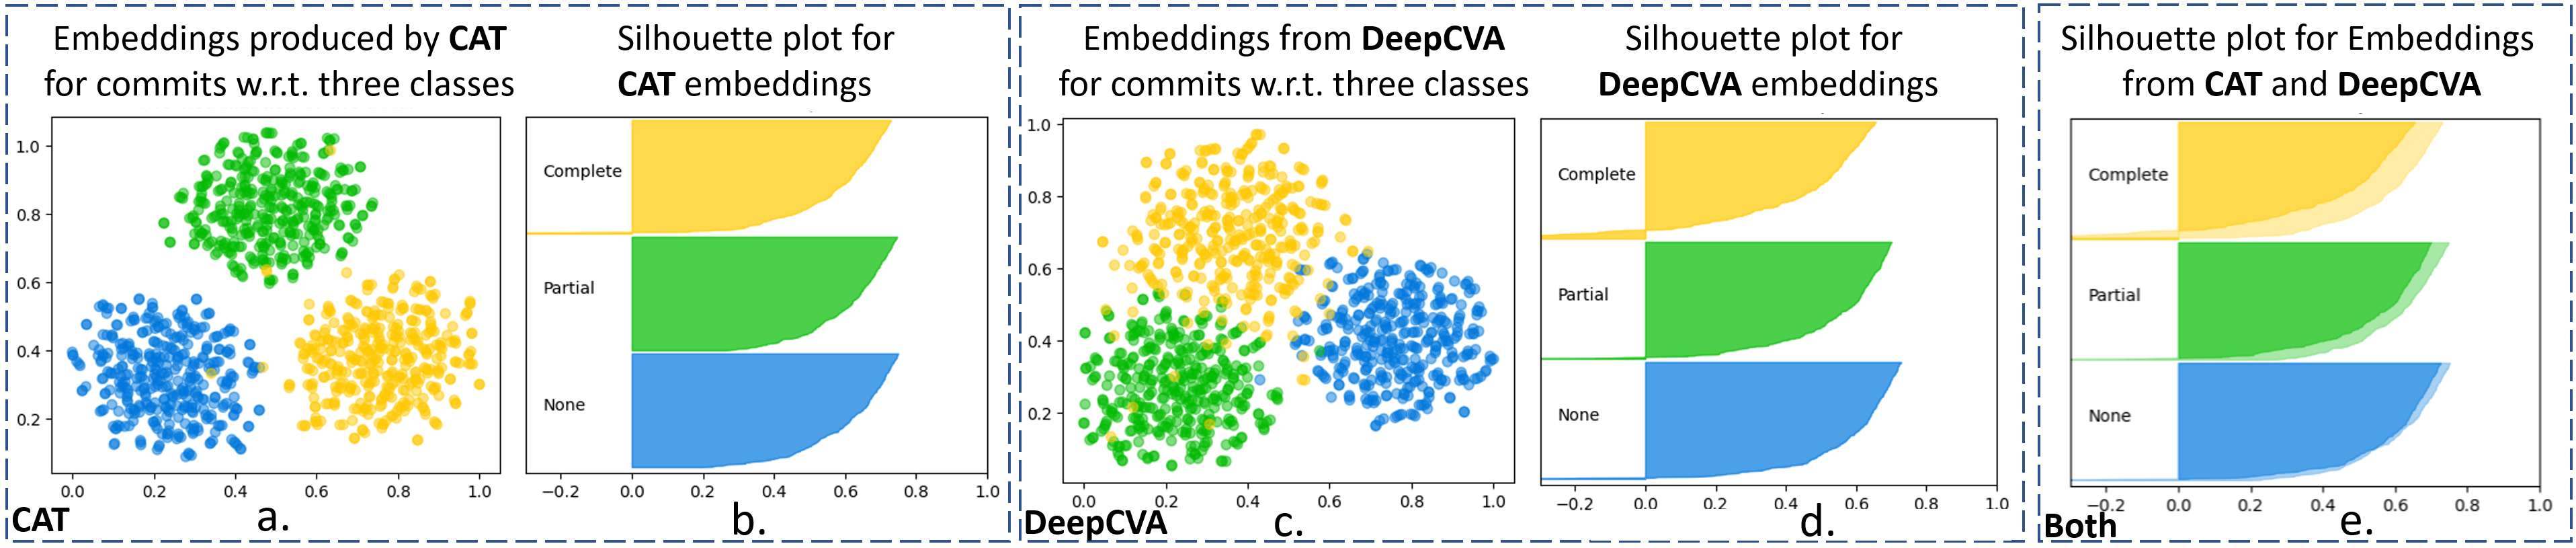
\includegraphics[width=6.9in]{graphs/confidentiality}
        \vspace{-6pt}
	\caption{Silhouette Plots for the Embeddings of Commits produced by {\tool} and DeepCVA regarding CONFIDENTIALITY}
	\label{fig:confidentiality}
\end{figure*}

%\begin{figure*}[t]
%	\centering
%	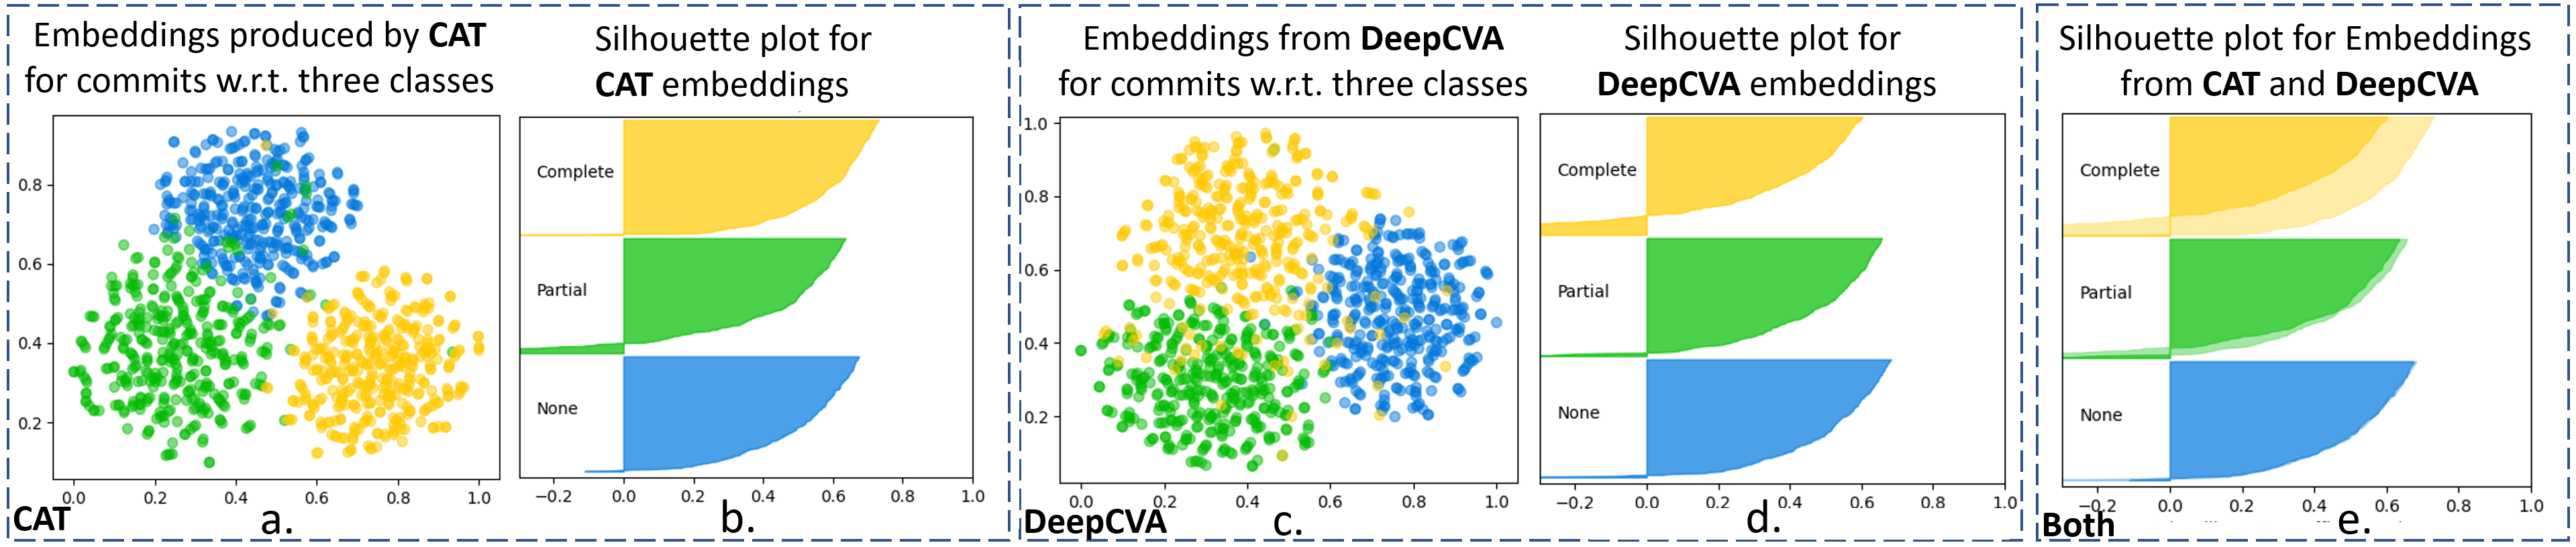
\includegraphics[width=6.9in]{graphs/integrity}
%        \vspace{-6pt}
%	\caption{Silhouette Plots for the Embeddings of Commits produced by {\tool} and DeepCVA regarding INTEGRITY}
%	\label{fig:integrity}
%\end{figure*}

\begin{figure*}[t]
	\centering
	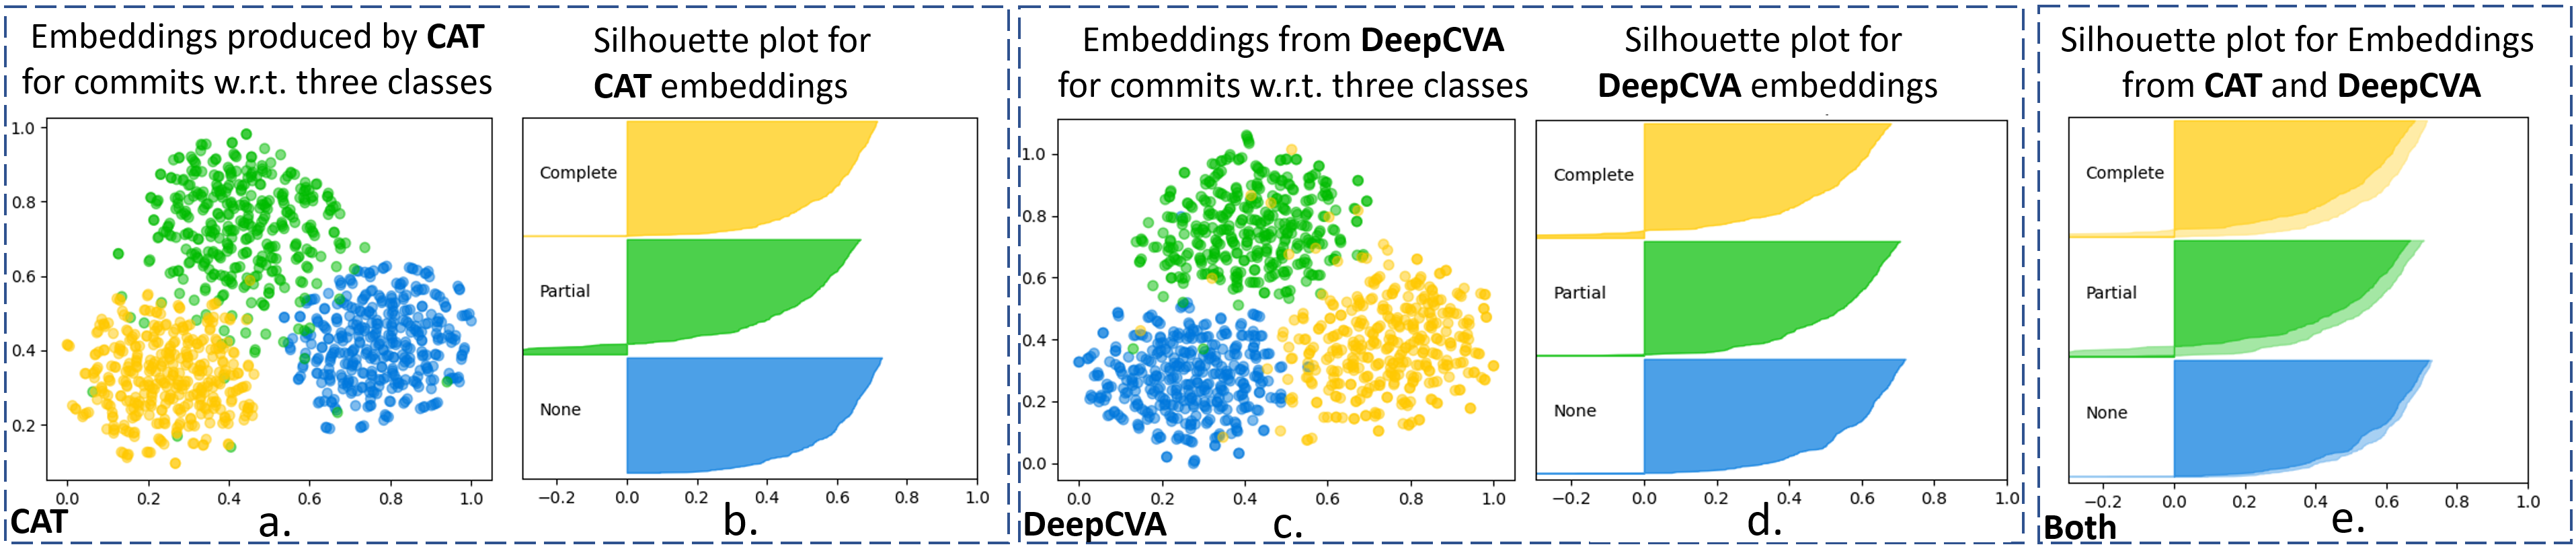
\includegraphics[width=6.9in]{graphs/availability}
       \vspace{-6pt}
	\caption{Silhouette Plots for the Embeddings of Commits produced by {\tool} and DeepCVA regarding AVAILABLITY}
	\label{fig:availability}
\end{figure*}

%
%\begin{figure*}[t]
%	\centering
%	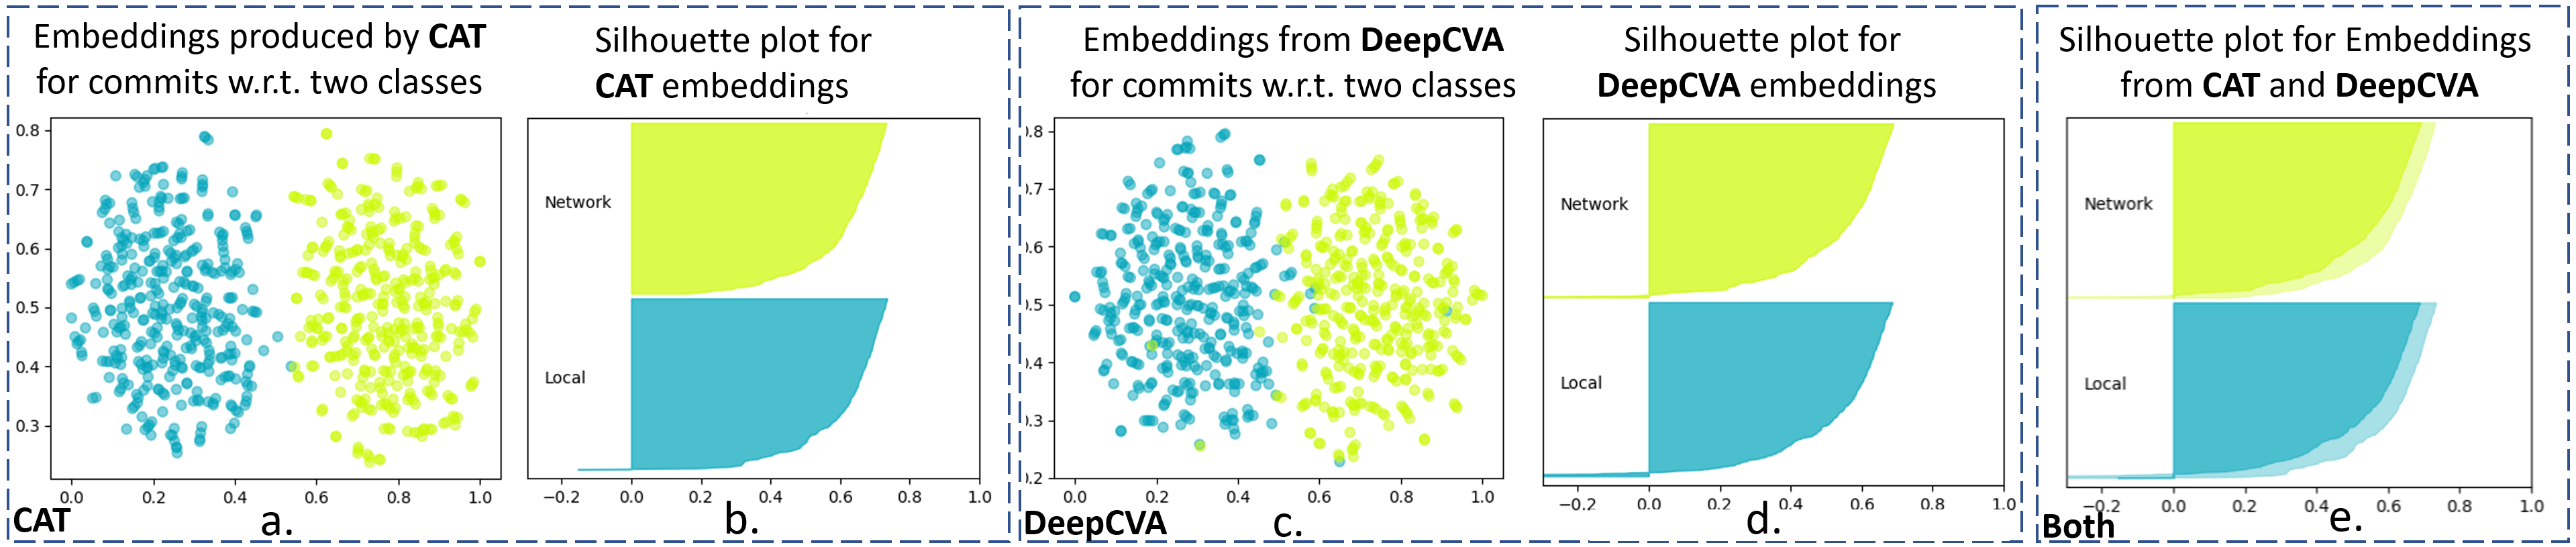
\includegraphics[width=6.9in]{graphs/access-vector}
%        \vspace{-6pt}
%	\caption{Silhouette Plots for the Embeddings of Commits produced by {\tool} and DeepCVA regarding ACCESS VECTOR}
%	\label{fig:access-vector}
%\end{figure*}

%\begin{figure*}[t]
%	\centering
%	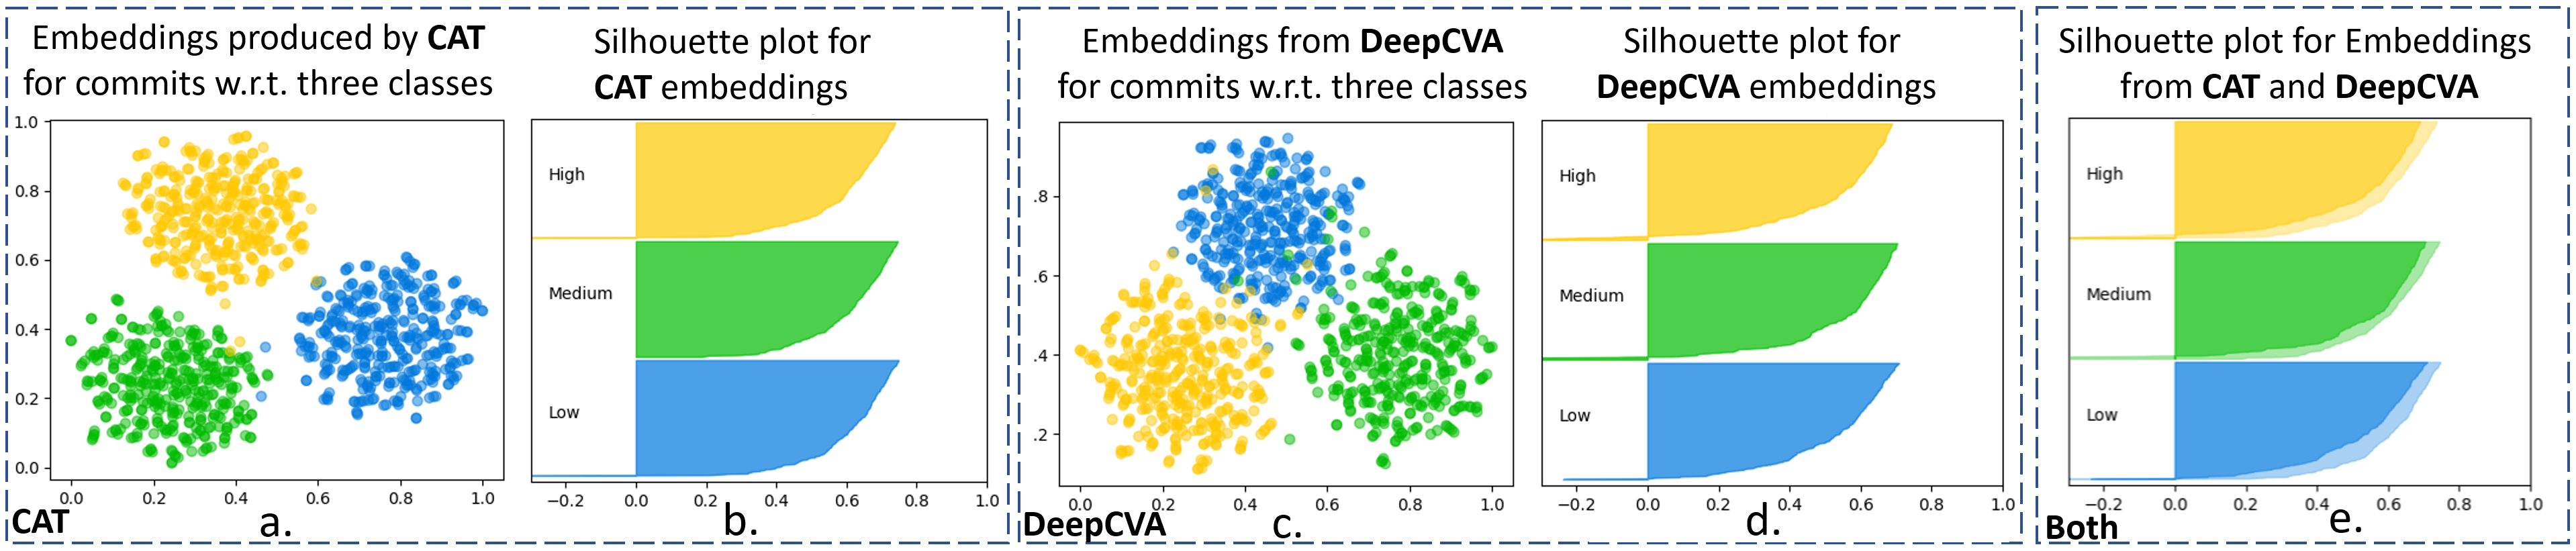
\includegraphics[width=6.9in]{graphs/access-complexity}
%        \vspace{-6pt}
%	\caption{Silhouette Plots for the Embeddings of Commits produced by {\tool} and DeepCVA regarding ACCESS COMPLEXITY}
%	\label{fig:access-complexity}
%\end{figure*}

%\begin{figure*}[t]
%	\centering
%	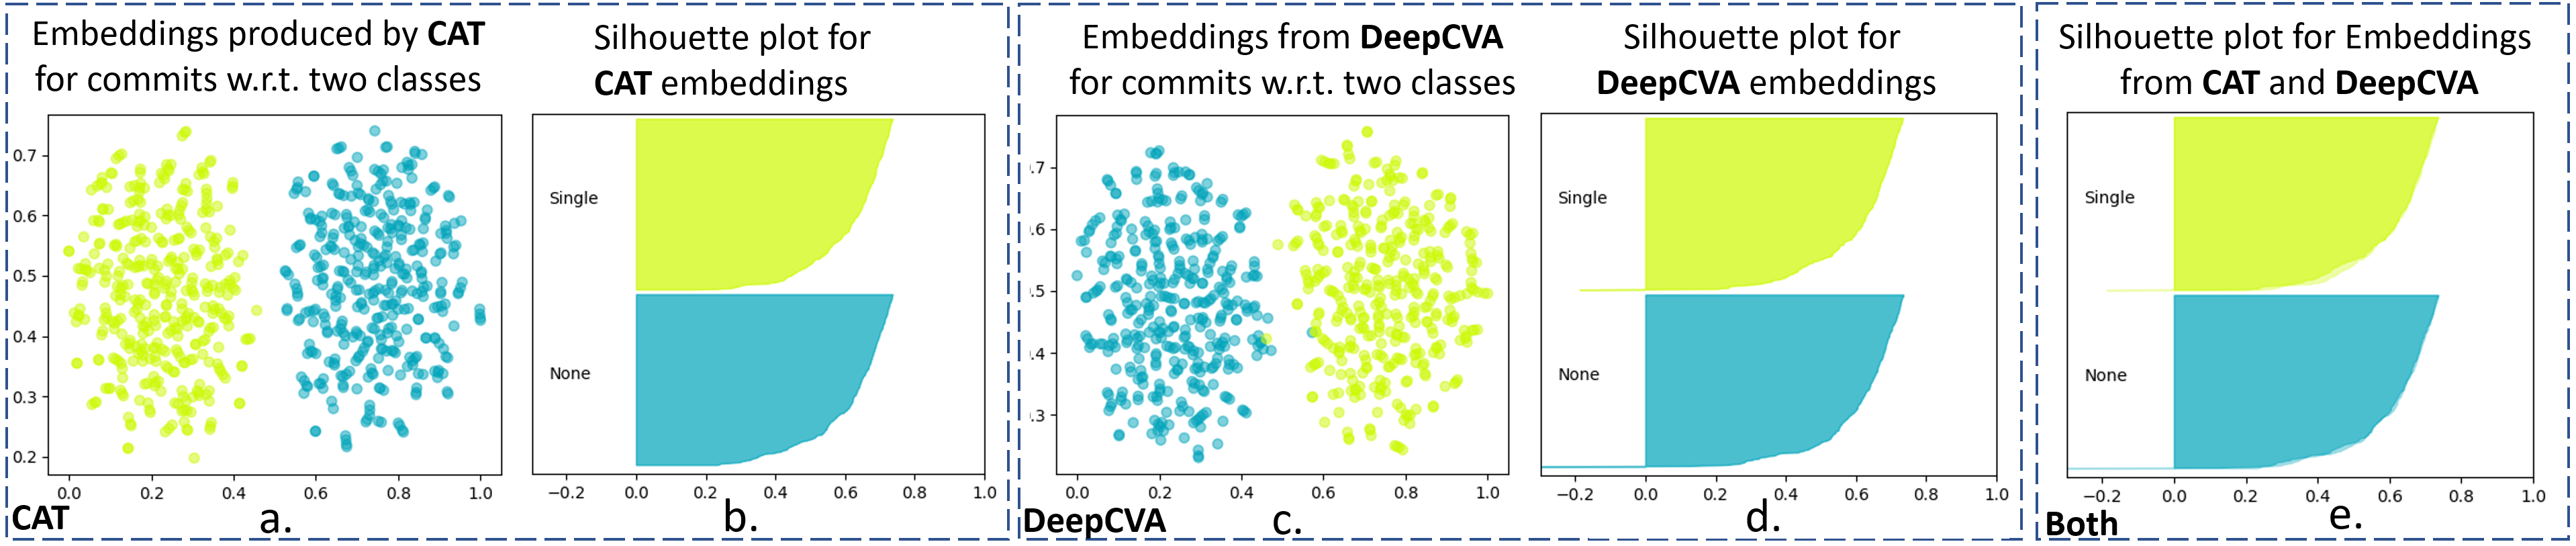
\includegraphics[width=6.9in]{graphs/authentication}
%        \vspace{-6pt}
%	\caption{Silhouette Plots for the Embeddings of Commits produced by {\tool} and DeepCVA regarding AUTHENTICATION}
%	\label{fig:authentication}
%\end{figure*}

%\begin{figure*}[t]
%	\centering
%	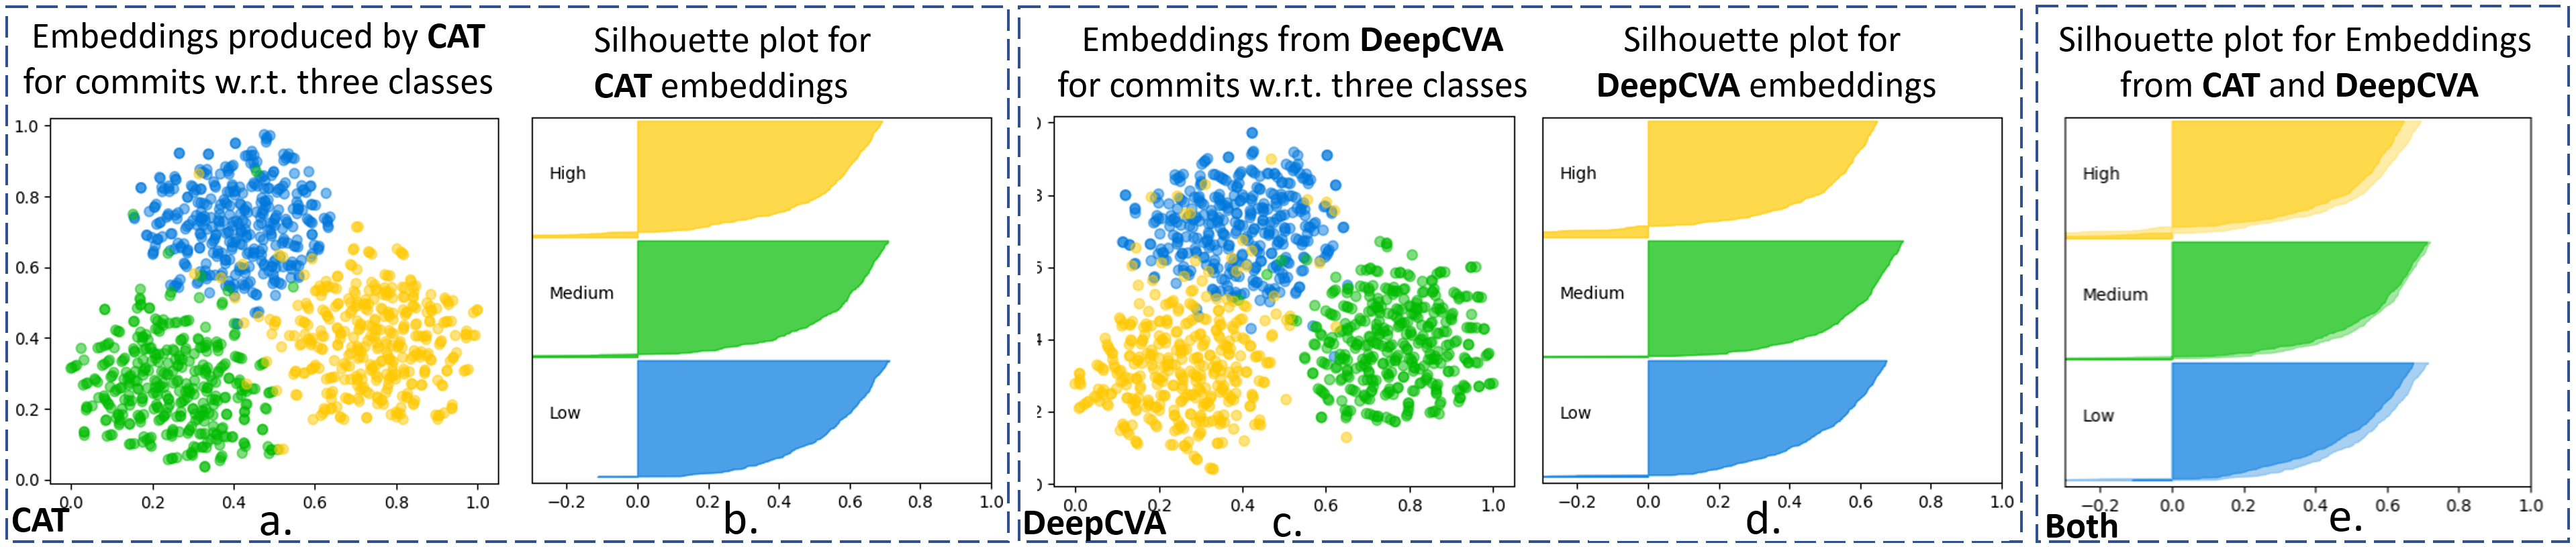
\includegraphics[width=6.9in]{graphs/severity}
%        \vspace{-6pt}
%	\caption{Silhouette Plots for the Embeddings of Commits produced by {\tool} and DeepCVA regarding SEVERITY}
%	\label{fig:severity}
%\end{figure*}

%We first processed each vulnerability assessment type (VAT).

In this study, we aim to show that our {\em embeddings for code
changes helps {\tool} have better class-separation}, i.e., {\em better
classification} in detection/assessment, than the baseline's.

%In this experiment, we aim to show that our novel graph-based, code
%change embeddings help {\tool} perform better classification for the
%grades in vulnerability assessment types than the $n$-gram-based
%embeddings in the baseline approach. We aim to show that the
%embeddings from {\tool} helps it have better class-separation, leading
%to better detection/assessment.

For each class~$C$ regarding a vulnerability assessment type (VAT), we
selected 366 commits that are labeled with the class $C$ in the
oracle. For example, for {\em Confidentiality}, we randomly selected
366 commits that are marked as {\em None}, 366 commits marked as {\em
Partial}, and 366 commits marked as {\em Complete}. Since our study
does not depend on the distribution across classes, we chose the same
number of samples for a class. Given the population of our data, that
sample size gives the confidence level of 95\% and the confidence
interval of 5\% for a~VAT.
%
For each type, we took those 366 $\times$ 3 = 1,098 commits and used
{\em {\tool}'s code change representation learning model} and {\em DeepCVA's
$n$-gram-based embedding model} to produce the embeddings for
those commits.  We projected the embeddings from two models
into the vector space using t-SNE technique. t-SNE~\cite{tsne}~is~a
statistical method for visualizing high-dimensional data by giving
each data point its projected location in a two-dimensional vector
space. We used the silhouette plot~\cite{silhouette-plot} to
present the data points for those embeddings. The silhouette plot
provides a succinct graphical view of how well the data points have
been classified.

Figure~\ref{fig:confidentiality} shows the comparison between the
silhouette plots for the embeddings produced by {\tool} and DeepCVA
regarding 3 classes of
Confidentiality. Figures~\ref{fig:confidentiality}a. and c. display
the t-SNE visualizations for the embeddings.
%produced by {\tool} and DeepCVA, respectively.
Figures~\ref{fig:confidentiality}b. and d. display the silhouette
plots for the data in the t-SNE visualization.
%for {\tool} and DeepCVA.
The silhouette coefficient value ($X$-axis in
Figures~\ref{fig:confidentiality}b., d., e.) is a measure of how
similar an object is to its own class compared to~other classes. The
silhouette coefficient value is in [-1,1], where a high value
indicates that an object is well matched to~its own class and poorly
matched to neighboring classes. If most objects have high values, the
class configuration is proper. That corresponds
to better-formed classes, facilitating a model to group the commits
into the correct classes ({\em None, Partial, Complete)}.
%regarding Confidentiality.
If many points have low or negative values, the
class configuration is poor-formed, which do not help in
classification.

Let us consider the commits in the {\em Complete} class
in~Figures \ref{fig:confidentiality}a. and b. Each line in the {\em
Complete} class in Figure~\ref{fig:confidentiality}b. corresponds to a
point in the {\em Complete} class in the vector space in
Figure~\ref{fig:confidentiality}a. The length of the line is equal to
the silhouette coefficient for a point. The lines are
sorted from largest to smallest and drawn from top to bottom, creating
a knife shape.

As seen, the knife shapes from DeepCVA have longer and thicker
tails than the ones from {\tool}, which actually have no tail for the
classes {\em Partial} and {\em None}. This means that DeepCVA produces
those embeddings that are not well-matched with its own classes and
mixed with the embeddings of the neighboring classes. In
Figure~\ref{fig:confidentiality}e., we place two silhouette plots in
an overlay image. The plot from {\tool} is thicker than that from
DeepCVA: {\tool} produces more points with positive values than
DeepCVA. In brief, Figures~\ref{fig:confidentiality}a--e show that the
{\em embeddings for code changes from {\tool} facilitates better
classification for VA than the embeddings from DeepCVA}.

%~\ref{fig:access-vector},
%~\ref{fig:access-complexity},
%~\ref{fig:authentication},

%Figures~\ref{fig:integrity},~\ref{fig:availability},
%and~\ref{fig:severity}

Figure~\ref{fig:availability} shows the comparison among the
silhouette plots for the embeddings from {\tool} and DeepCVA on
Availability (The ones for others are not shown due to space limit).
As seen, the comparisons for the VATs have the same trend. The knife
shapes from {\tool} have no or shorter tails and are thicker than
those of DeepCVA.

In brief, the silhouette plots indicate that {\tool} produces the
embeddings that have more cohesion with the ones in the same class and
more separation with the ones in the different classes. Thus, our {\bf
embeddings with more class-separability help {\tool} perform better
classification for VA}.

%regarding each vulnerability assessment type}.


\begin{figure}[t]
	\centering
	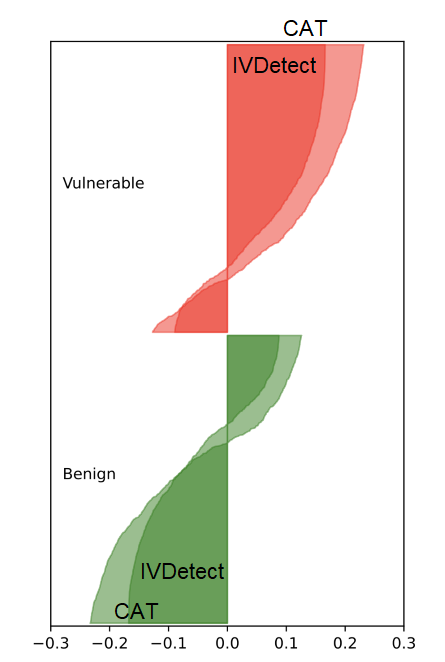
\includegraphics[width=1.4in]{graphs/plot-vd}
       \vspace{-6pt}
	\caption{Silhouette Plots for the Embeddings of Commits produced by {\tool} and DeepCVA for Vulnerability Detection: {\tool} has better Class Separability}
	\label{fig:vd}
\end{figure}

We also performed the same plotting for the classification task for
vulnerability detection. Considering the overlap between two plots in
Figure~\ref{fig:vd}, the knife shapes from {\tool} for both classes
(vulnerability and benign) are wider and have less negative values
than those from the best baseline IVDetect. Specifically, the average
silhouette score in {\tool} is 0.027, while that of IVDetect is
0.0072. Thus, this result shows that {\tool} has better
class-separability, leading to better performance than the baseline
model.

\subsubsection{\bf Class Separability with Code Change Embeddings (RQ3)}
\label{sec:separation}

%\subsubsection{\bf Contribution of Code Change Embeddings in Classification (RQ3)}

\begin{figure*}[t]
	\centering
	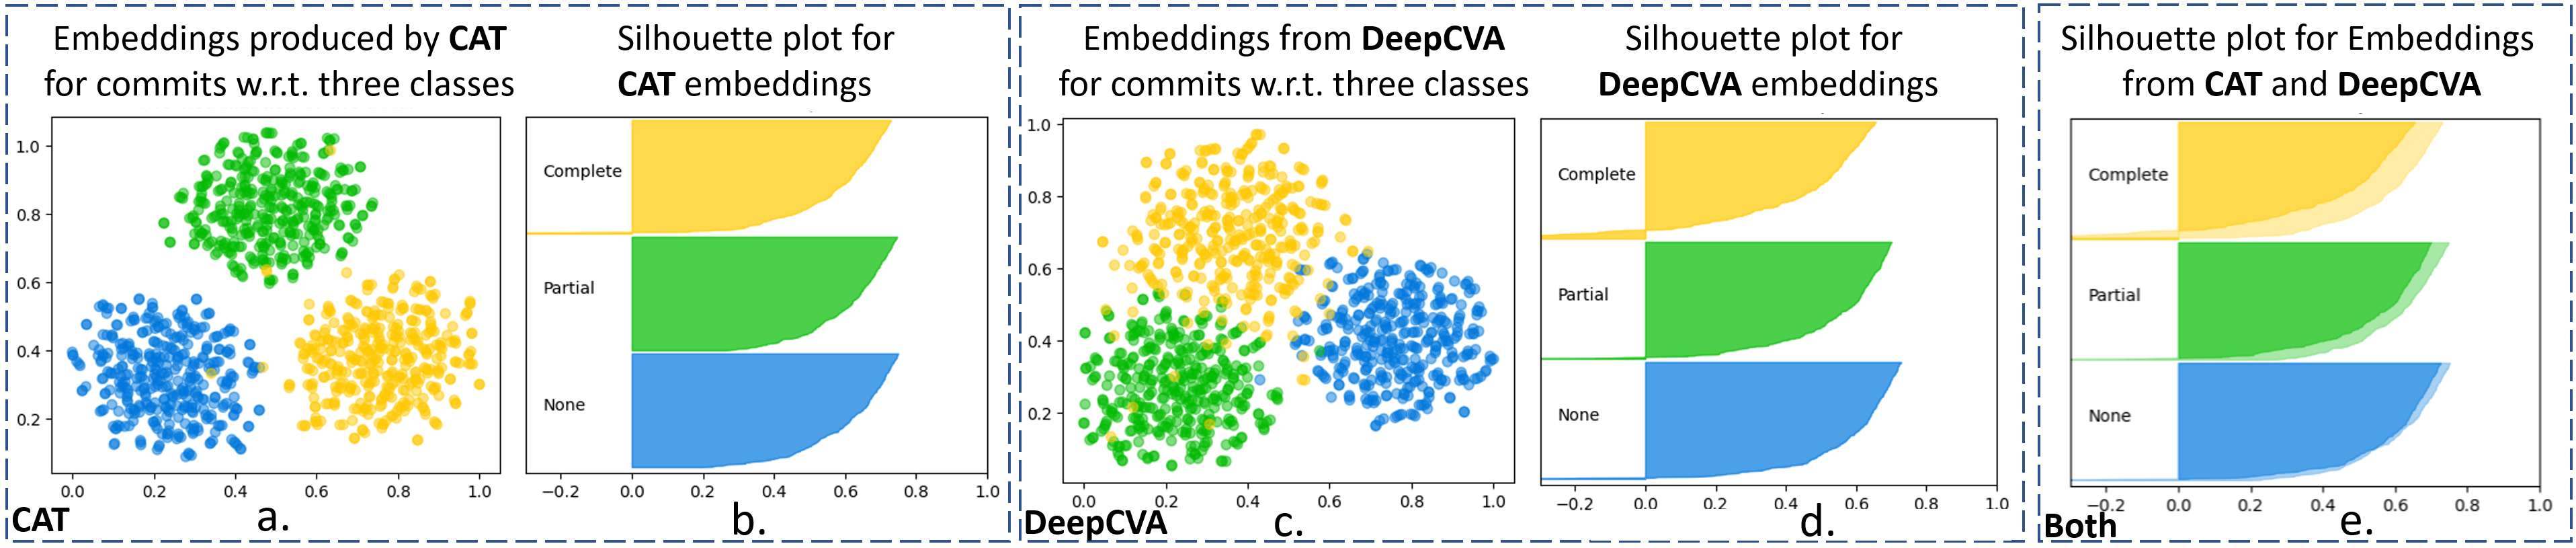
\includegraphics[width=6.9in]{graphs/confidentiality}
        \vspace{-6pt}
	\caption{Silhouette Plots for the Embeddings of Commits produced by {\tool} and DeepCVA regarding CONFIDENTIALITY}
	\label{fig:confidentiality}
\end{figure*}

%\begin{figure*}[t]
%	\centering
%	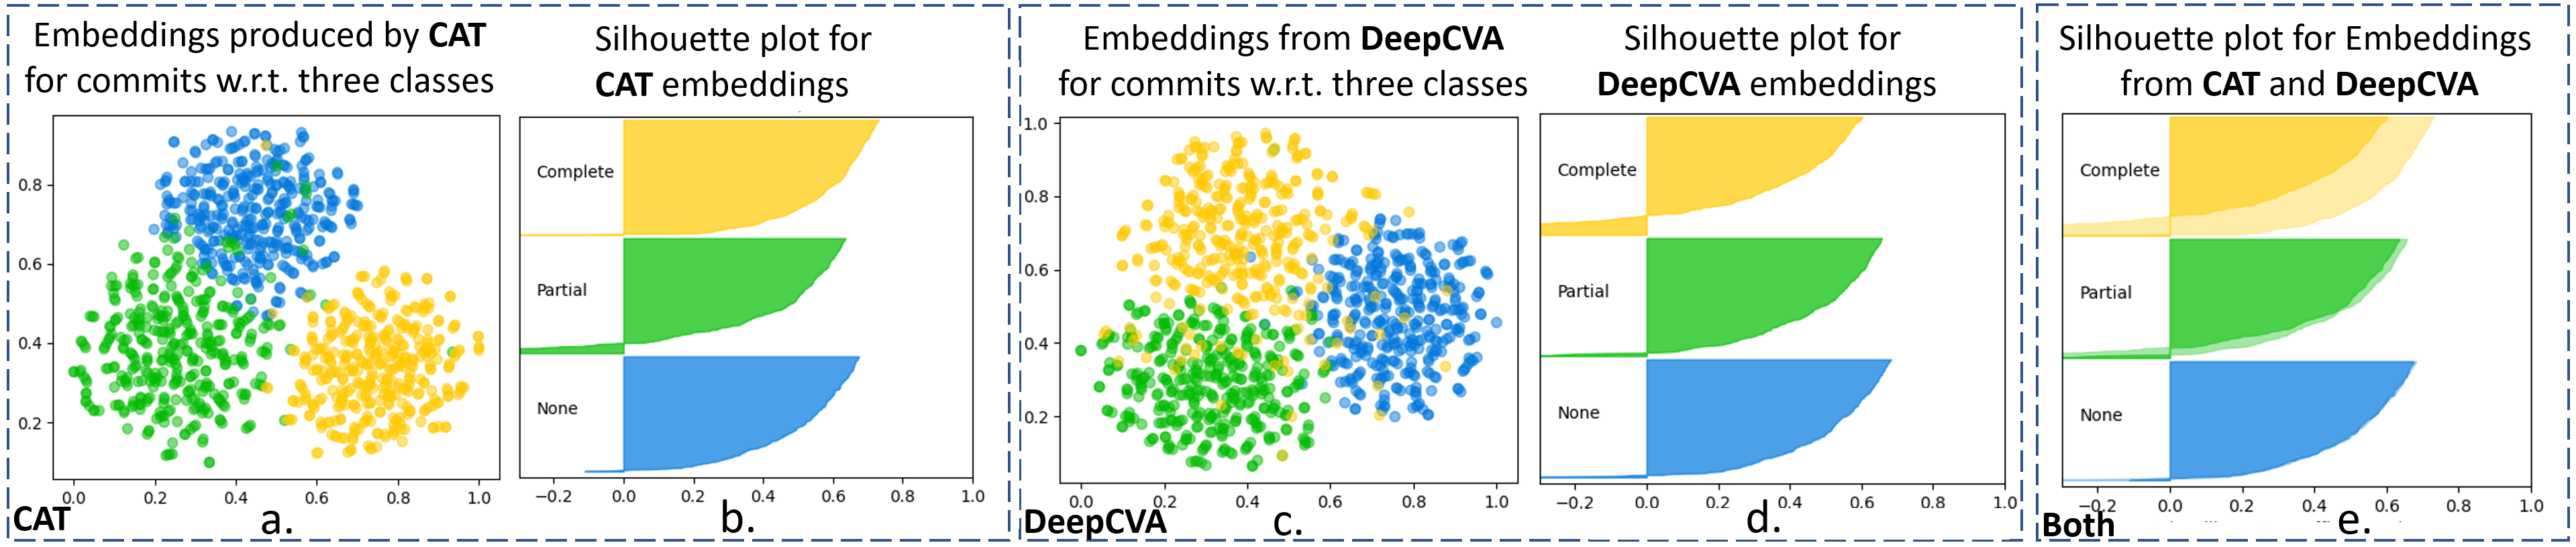
\includegraphics[width=6.9in]{graphs/integrity}
%        \vspace{-6pt}
%	\caption{Silhouette Plots for the Embeddings of Commits produced by {\tool} and DeepCVA regarding INTEGRITY}
%	\label{fig:integrity}
%\end{figure*}

\begin{figure*}[t]
	\centering
	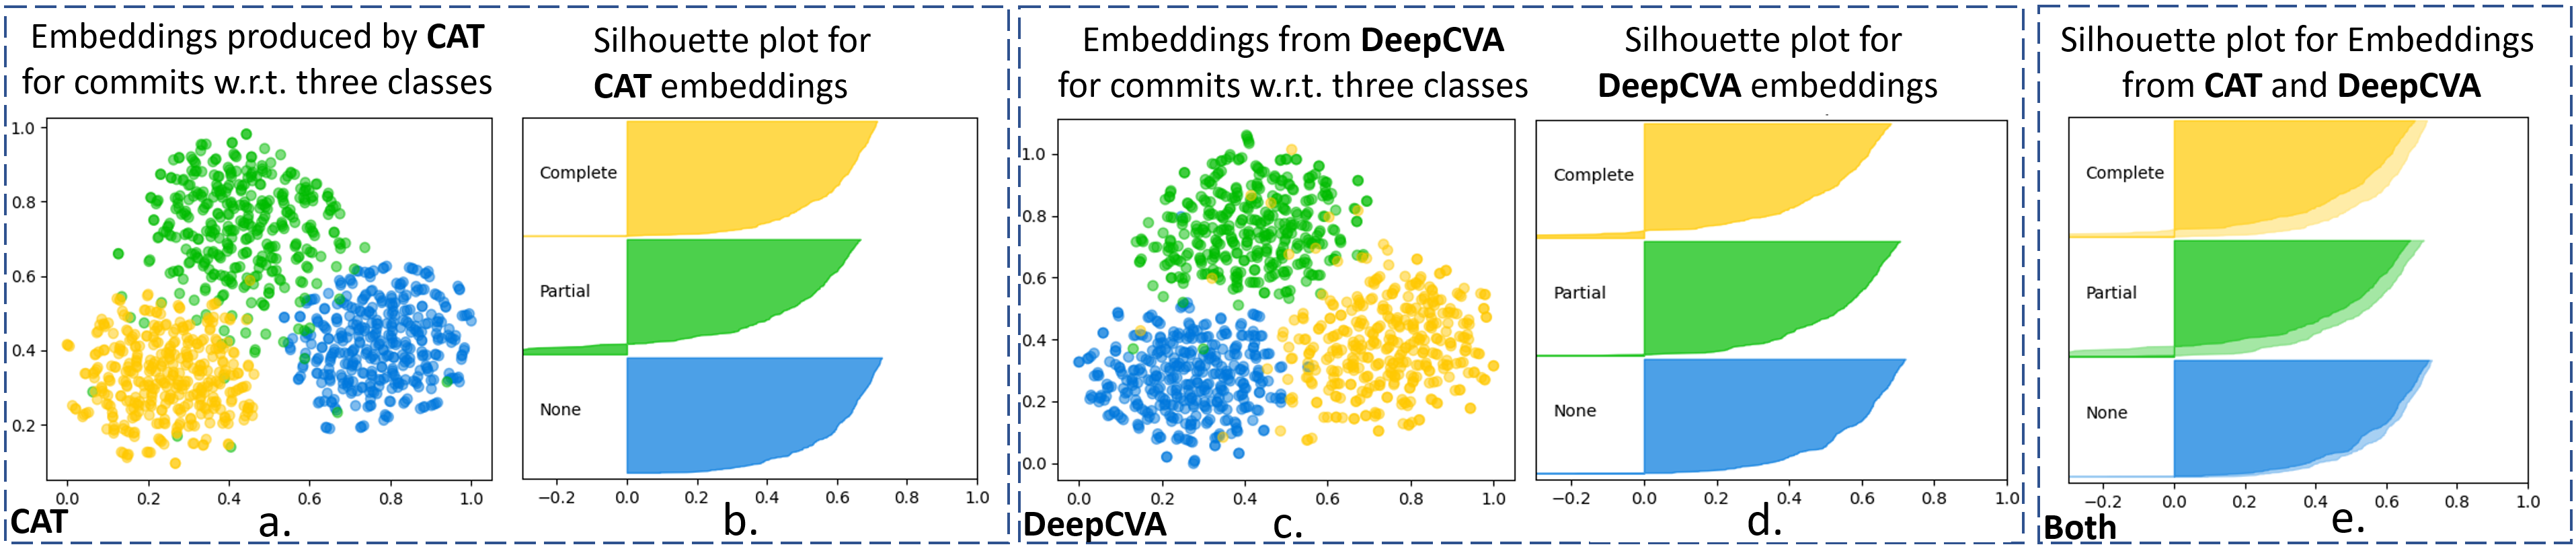
\includegraphics[width=6.9in]{graphs/availability}
       \vspace{-6pt}
	\caption{Silhouette Plots for the Embeddings of Commits produced by {\tool} and DeepCVA regarding AVAILABLITY}
	\label{fig:availability}
\end{figure*}

%
%\begin{figure*}[t]
%	\centering
%	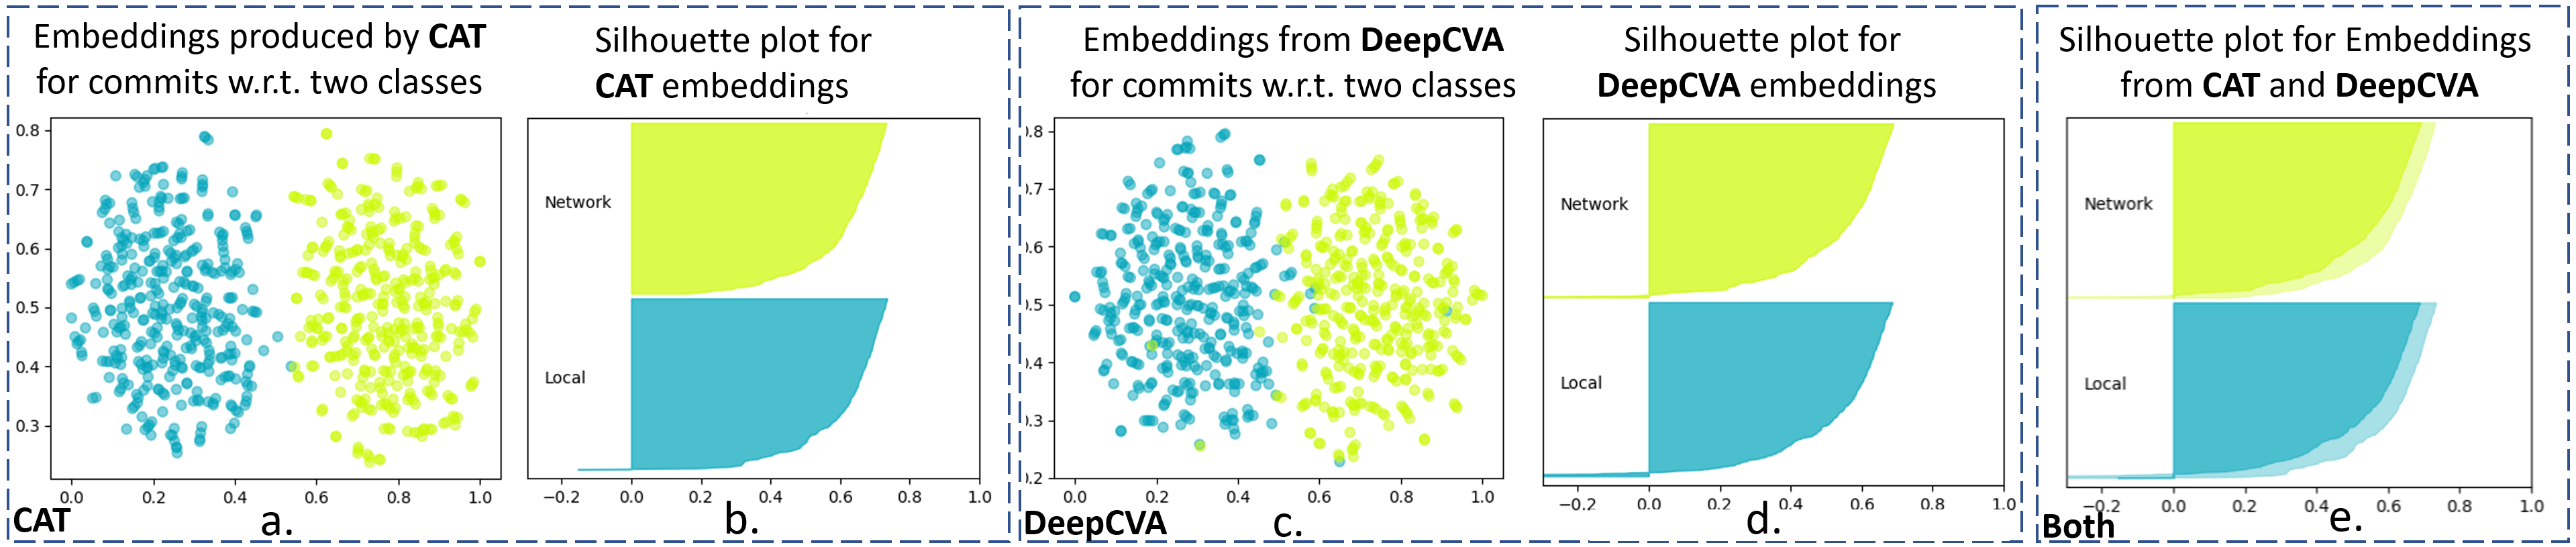
\includegraphics[width=6.9in]{graphs/access-vector}
%        \vspace{-6pt}
%	\caption{Silhouette Plots for the Embeddings of Commits produced by {\tool} and DeepCVA regarding ACCESS VECTOR}
%	\label{fig:access-vector}
%\end{figure*}

%\begin{figure*}[t]
%	\centering
%	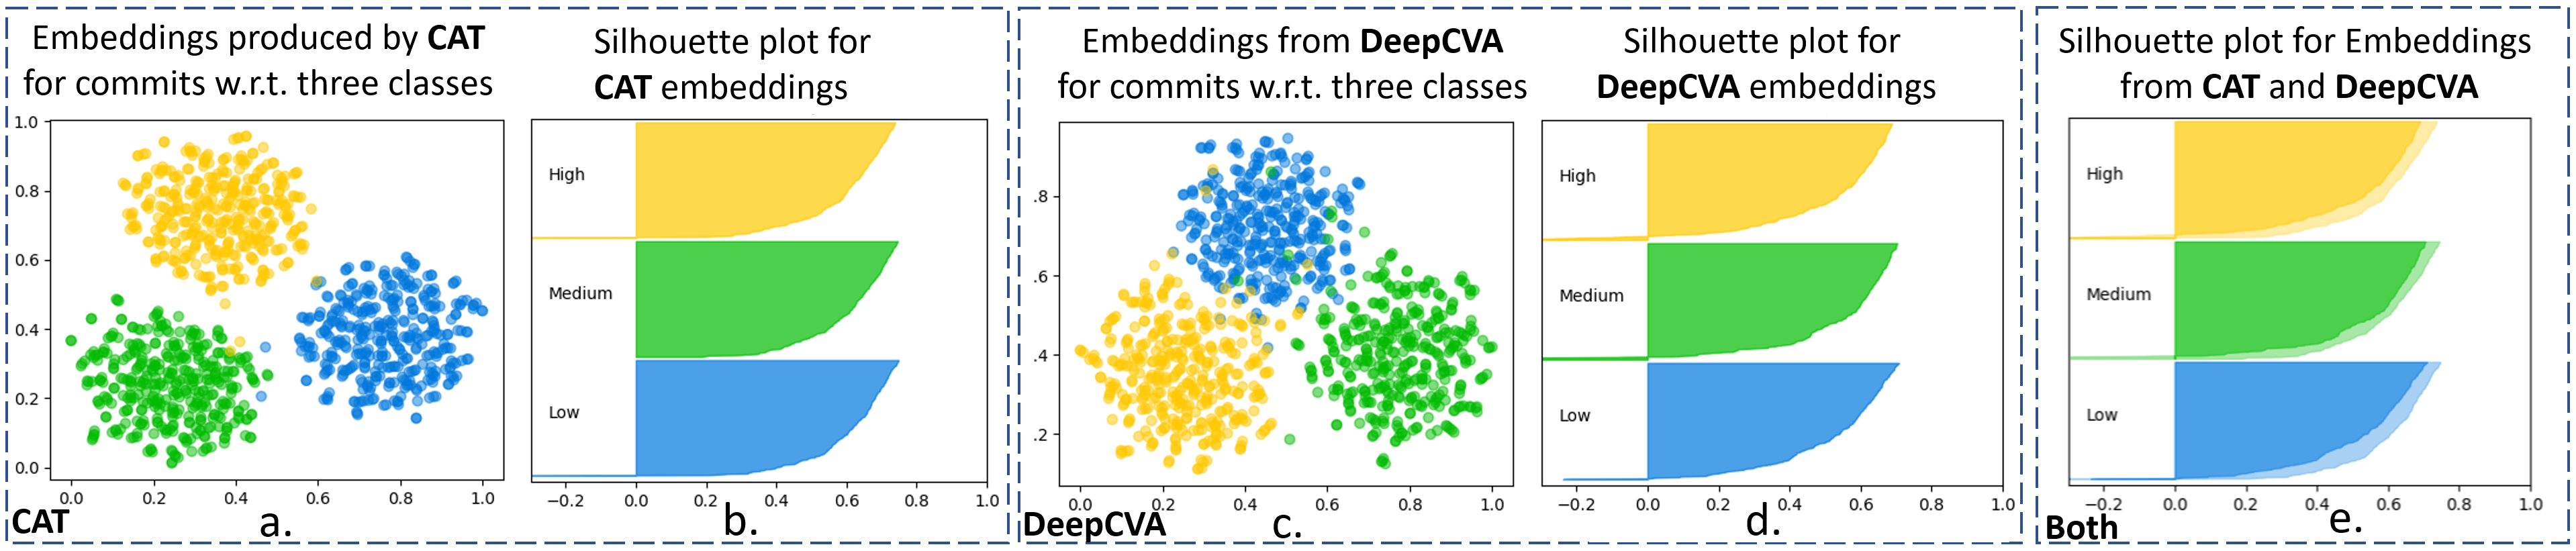
\includegraphics[width=6.9in]{graphs/access-complexity}
%        \vspace{-6pt}
%	\caption{Silhouette Plots for the Embeddings of Commits produced by {\tool} and DeepCVA regarding ACCESS COMPLEXITY}
%	\label{fig:access-complexity}
%\end{figure*}

%\begin{figure*}[t]
%	\centering
%	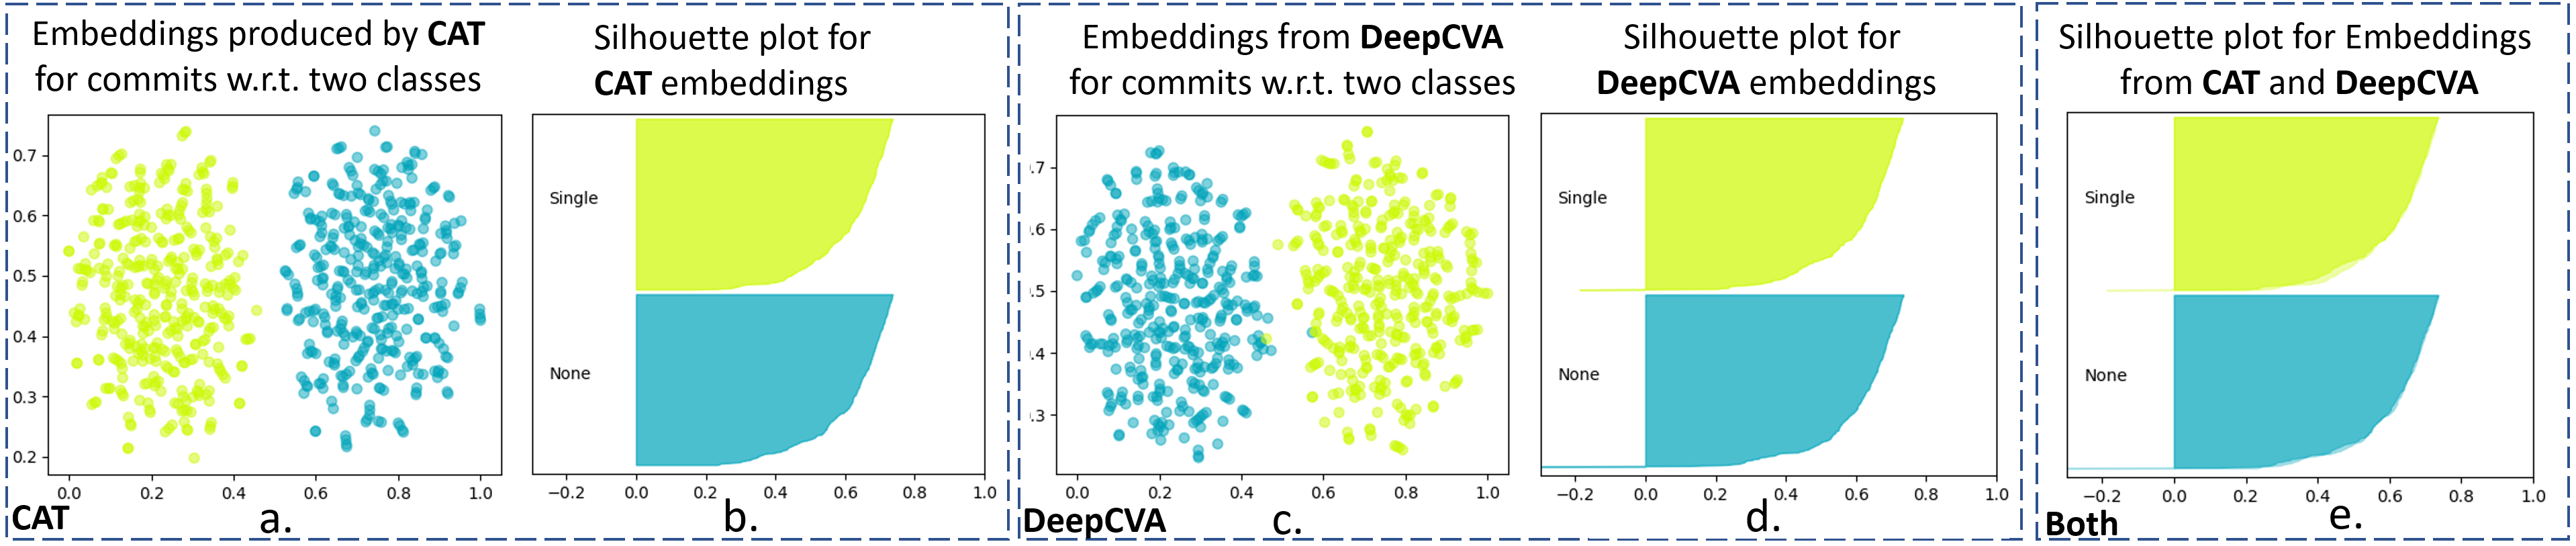
\includegraphics[width=6.9in]{graphs/authentication}
%        \vspace{-6pt}
%	\caption{Silhouette Plots for the Embeddings of Commits produced by {\tool} and DeepCVA regarding AUTHENTICATION}
%	\label{fig:authentication}
%\end{figure*}

%\begin{figure*}[t]
%	\centering
%	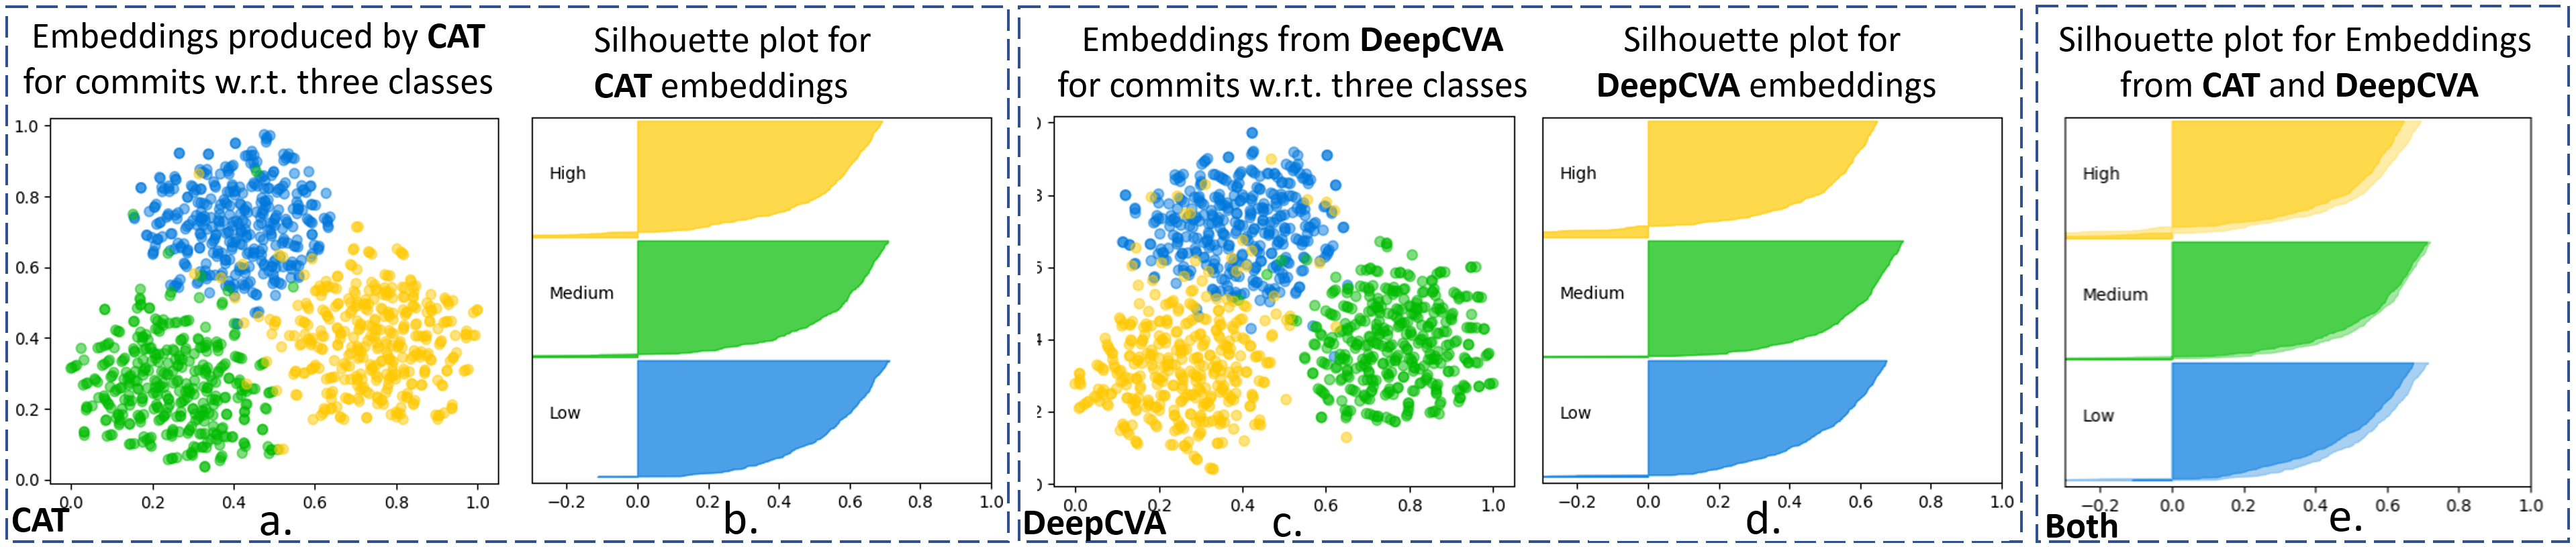
\includegraphics[width=6.9in]{graphs/severity}
%        \vspace{-6pt}
%	\caption{Silhouette Plots for the Embeddings of Commits produced by {\tool} and DeepCVA regarding SEVERITY}
%	\label{fig:severity}
%\end{figure*}

%We first processed each vulnerability assessment type (VAT).

In this study, we aim to show that our {\em embeddings for code
changes helps {\tool} have better class-separation}, i.e., {\em better
classification measures} for detection and assessment than that of the baseline.

%In this experiment, we aim to show that our novel graph-based, code
%change embeddings help {\tool} perform better classification for the
%grades in vulnerability assessment types than the $n$-gram-based
%embeddings in the baseline approach. We aim to show that the
%embeddings from {\tool} helps it have better class-separation, leading
%to better detection/assessment.

For each class~$C$ regarding a vulnerability assessment type (VAT), we
selected 366 commits that are labeled with the class $C$ in the
oracle. This was chosen based on the population of the data, such that the sample size corresponded to a 95\% confidence level, with a confidence interval of 5\% for each VAT. 
For example, for {\em Confidentiality}, we randomly selected
an equal number of commits (i.e., 366), that are marked as {\em None}, {\em Partial}, and {\em Complete}.
%Since our study
%does not depend on the distribution across classes, we chose the same
%number of samples for a class. The sample size, i.e., 366, was chosen based on the population of our data, and a , and a corresponding confidence interval of 
For each type, we took those 366 $\times$ 3 = 1,098 commits and used
{\em {\tool}'s code change representation learning model} and {\em DeepCVA's
$n$-gram-based embedding model} to produce the embeddings for
those commits.  We projected the embeddings from these approaches
into the vector space using t-SNE~\cite{tsne} technique, based on which we can visualize high-dimensional data by giving
each data point its projected location in a two-dimensional vector
space. Next, in the silhouette plots~\cite{silhouette-plot}, we succinctly present the data points for these embeddings, which represent how well they have
been classified.

Figure~\ref{fig:confidentiality} shows the comparison between the
silhouette plots for the embeddings produced by {\tool} and DeepCVA
regarding 3 classes of
Confidentiality. Figures~\ref{fig:confidentiality}a. and c. display
the t-SNE visualizations for the embeddings, while
%produced by {\tool} and DeepCVA, respectively.
figures~\ref{fig:confidentiality}b. and d. display the silhouette
plots for the data in these visualizations.
%for {\tool} and DeepCVA.
The silhouette coefficient value ($X$-axis in
Figures~\ref{fig:confidentiality}b., d., e.) is a measure of how
similar an object is to its own class compared to~other classes, which ranges from [-1, 1]. Here, a higher value
indicates that an object is well matched to~its own class and poorly
matched to neighboring classes. If most objects have high values, the
class configuration is proper. That corresponds
to better-formed classes, facilitating a model to group the commits
into the correct classes (i.e., {\em None, Partial,} and {\em Complete}).
If many points have low or negative values, the
class configuration is ill-formed, which does not help with
classification.

Let us consider the commits in the {\em Complete} class
in~Figures \ref{fig:confidentiality}a. and b. Each line in {\em
Complete} class in Figure~\ref{fig:confidentiality}b. corresponds to a
point in {\em Complete} class in the vector space in
Figure~\ref{fig:confidentiality}a. Length of a line is equal to
the silhouette coefficient for a point. These lines are
sorted from largest to smallest, and drawn from top to bottom, creating
a knife shape. As seen, the knife shapes from DeepCVA have longer and thicker
tails than those from {\tool}, which actually have no tail for the
classes {\em Partial} and {\em None}. 
%This means that DeepCVA produces
%those embeddings that are not well-matched with its own classes and
%mixed with the embeddings of the neighboring classes. 
%This means that 
Thus, DeepCVA produces
embeddings that overlap more with their neighboring classes.
In
Figure~\ref{fig:confidentiality}e., we place two silhouette plots in
an overlay image. The plot from {\tool} is thicker than that from
DeepCVA: {\tool} produces more points with positive values than
DeepCVA. In brief, Figures~\ref{fig:confidentiality}a--e show that the
{\em embeddings for code changes from {\tool} facilitates better
classification for VA than those from DeepCVA}.

%~\ref{fig:access-vector},
%~\ref{fig:access-complexity},
%~\ref{fig:authentication},

%Figures~\ref{fig:integrity},~\ref{fig:availability},
%and~\ref{fig:severity}

Figure~\ref{fig:availability} shows the comparison among the
silhouette plots for the embeddings from {\tool} and DeepCVA on
{\em Availability} (remaining VAT types are not shown here due to space limit).
We can see that the comparisons for all VATs have the same trend, i.e., the knife
shapes from {\tool} have no or shorter tails, and are thicker than
those of DeepCVA. In brief, the silhouette plots indicate that {\tool} produces 
embeddings that have more cohesion with the ones in the same class and
more separation with the ones in the different classes. Thus, our {\bf
embeddings with more class-separability help {\tool} perform better
classification for VA}.

%regarding each vulnerability assessment type}.


\begin{figure}[t]
	\centering
	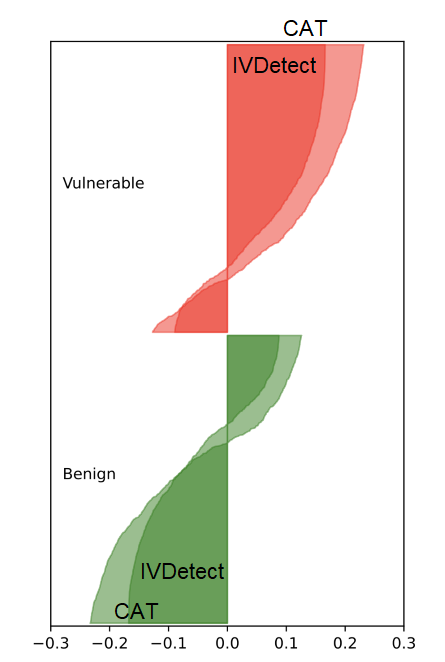
\includegraphics[width=1.3in]{graphs/plot-vd}
       \vspace{-6pt}
	\caption{Silhouette Plots for the Embeddings of Commits produced by {\tool} and DeepCVA for Vulnerability Detection: {\tool} has better Class Separability}
	\label{fig:vd}
\end{figure}

We also performed the same plotting for the classification task for
vulnerability detection. Considering the overlap between two plots in
Figure~\ref{fig:vd}, the knife shapes from {\tool} for both classes
(vulnerability and benign) are wider and have less negative values
than those from the best baseline IVDetect. Specifically, the average
silhouette score in {\tool} is 0.027, while that of IVDetect is
0.0072. Thus, {\tool} has better class-separability, leading to better
performance.

%\subsection{Discussion and Implications}

%\subsubsection{Using Explainable AI to explain the graph as the key features in {\tool}}

\subsubsection{{\bf Using Explainable AI to Study Relevant Features in Classification regarding Program Dependencies (RQ4)}}
\label{sec:ai}

%\subsubsection*{Using Explainable AI to explain the graph as the key features in {\tool}}

%{\tool} has two key ideas (Section~\ref{key-ideas:sec}) in advancing
%the state-of-the-art commit-level vulnerability assessment: 1)
%graph-based code change representation learning for program
%dependencies; and 2) contextualized embeddings for code changes. As
%seen in RQ5, our context-aware, graph-based, representation learning
%(RL) model produces the embeddings for the code changes in the
%commits that facilitate {\tool} in better classifying the
%commit-level changes into more correct classes regarding  the assessment
%types than DeepCVA~\cite{deepCVA-ase21}.
We aim to evaluate whether {\tool} uses the vulnerable statements
and their dependencies in its vulnerability prediction and
assessment. This also allows us to evaluate its ability to pinpoint
the changed statements relevant to the detected vulnerability.
%capable of {\em capturing the key vulnerable statements and
%dependencies}, leading to its accuracy in vulnerability assessment.
Specifically, for each vulnerability assessment type (VAT), we
randomly selected 366 samples of the commits in our dataset that
{\tool} predicts the correct classes (e.g., {\em None}, {\em Partial},
{\em Complete}) of the vulnerability detection and VATs for them. That sample size gives us the confidence level of 95\% and
the confidence interval of 5\% for each VAT.

We use an explainable Artificial Intelligence (XAI) model,
called {\em GNNExplainer}~\cite{GNNExplainer}, which takes a GNN-based
classification model $\mathcal{M}$ and a specific input $I$ of
$\mathcal{M}$, and produces an explanation on why $\mathcal{M}$
arrives at its prediction $O$ for the input $I$.
%
We fed {\tool} and each commit $C$ of those sample commits as the
input for GNNExplainer. The explanation produced by GNNExplainer is in
the form of a sub-graph $\Delta$ in {\mvpdg} that was built from the
input commit $C$. The sub-graph $\Delta$ is referred to as the {\em
explanation sub-graph} for $C$ regarding the classification of $C$ for
the current assessment type. The explanation sub-graph $\Delta$ is
defined as the minimal sub-graph in the input graph {\mvpdg} that
minimizes the prediction scores between using the entire graph
{\mvpdg} and using $\Delta$ as the input for {\tool}. $\Delta$ is
minimal in the sense that if any node and edge is removed from it, the
decision of {\tool} is affected, i.e., {\tool} will produce a
different class for the input commit $C$. That is, {\em the
explanation sub-graph $\Delta$ contains the statements and
dependencies that are most decisive for {\tool} to determine the class
$O$ for the commit $C$}.

To evaluate whether {\tool} via Label-GCN can capture the crucial
statements and dependencies in deciding the class for an input commit,
%regarding an assessment type,
we compared the explanation sub-graph $\Delta$ with the
vulnerability-inducing statements and dependencies in the ground
truth of those commits. If $\Delta$ contains one of such statements
(nodes) and dependencies (edges), we consider that {\tool} uses the
correct vulnerable statements and dependencies as the features for its
correct classification (detection and assessment).
%regarding an assessment type.

%\textcolor{red}{As seen in Table~\ref{},...}

\begin{table}[t]
\caption{Vunerable Statements/Dependencies as Key Features}
	\vspace{-12pt}
	\tabcolsep 2.3pt
%	\footnotesize
\small
	\begin{center}
\begin{tabular}{|r|r|r|r|r|r|r||r|}
  \hline
     {\em Confidence} & {\em Integrity} & {\em Avail} & {\em AccessVec} & {\em AccCompl} & {\em Auth} & {\em Severity} & {\bf Avg} \\
  \hline
    63 & 84 & 81 & 72 & 93 & 93 & 81 & 81.4 \\
 % \% & 17 & 22 & 11 & 19 & 24.5 & 37 & 21 & 21.6 \\
  \hline
\end{tabular}
\label{gnn}
\%Commits {\tool} correctly uses vulnerable statements/dependencies in Vulnerability Detection and Assessment
\end{center}
\vspace{-12pt}
\end{table}

%\input{sections/code-example}

%N= \# of commits that \tool correctly uses the vulnerable statements and dependencies\\

%Table~\ref{gnn} shows us how much {\tool} uses the vulnerable statements and their dependencies in predicting the correct assessments. For example, among a sample of 366 commits that {\tool} successfully classified into {\em None} or {\em Single} for {\em Authentication}, there are 139 commits in which {\tool} uses the actual vulnerable statements and their dependencies in its prediction/assessment. GNNExplainer determines that {\tool} had made the correct classifications for {\em Authentication} because {\tool} used at least one of the actual vulnerable statements/dependencies. In other words, in 139 commits, {\tool} used the vulnerable statements/dependencies as its key features in the correct classifications. As seen, across different assessment types, the degree of {\tool}'s relying on the vulnerable statements and dependencies for its assessment is different. While only 11\% of the samples, {\tool} relies on vulnerable statements/dependencies to assess the impact of {\em Availability}, in 37\% of the samples, it relies on them for assessing that of {\em Authentication}. On average, in 21.6\% of the samples, {\tool} correctly relies on the vulnerable statements and their dependencies in vulnerability assessment. 

Table~\ref{gnn} shows how much {\tool} uses the vulnerable
statements and their dependencies in correctly predicting the
VATs. For example, among the 366 commits that {\tool} successfully
classified into ({\em None}, {\em Single}) for {\em Authentication},
GNNExplainer determines that in 93\% of them, {\tool}
uses the actual vulnerable statements and their dependencies as key
features in its prediction.
%GNNExplainer determines that {\tool} had made the correct
%classifications for {\em Authentication} because {\tool} used at least
%one of the actual vulnerable statements/dependencies.
%That is, in 139 commits, {\tool} used the vulnerable
%statements/dependencies as its key features in the correct
%classifications.
As seen, the degree of {\tool}'s
reliance on vulnerable statements/dependencies for its assessment
across different types
is different.  While in 84\%, {\tool} relies on vulnerable
statements/dependencies to assess the impact of {\em Integrity}; in
81\% samples, it relies on them for assessing that of {\em Severity}.
For {\em vulnerability detection}, in 84\% of samples, {\tool} uses
the right statements/dependencies in its correct prediction (not
shown).
%
On an average, in {\bf 81.4\%} samples, {\tool} correctly
relies on the vulnerable statements/dependencies.
%To correctly assess the remaining samples, {\tool} might use other
%features, e.g., contexts, code tokens, and the impacts of
%multiple~tasks.
In brief, this result shows that {\em program dependencies among
vulnerable statements are key features to {\tool} in its correct
vulnerability detection and assessment}.



%In the other 78.4\%, {\tool} uses other features for correct classifications. Even though the vulnerability-introducing statements and dependencies are not in the minimum sub-graphs from GNNExplainer. However, we found that in all of the 78.4\% cases, one or several statements in the minimum sub-graphs have direct dependencies with the vulnerability-introducing statements. 
%(but they are not directly connected). %The reason is that GNNExplainer, an approximation explanation model, is limited in generating only connected graphs as explanations, thus if the contributing features are a combination of a connected graph and a couple non-connected statements, then the non-connected ones will not be included in the sub-graphs. 




%automatic verification of 

%We can only automatically verify whether {\tool} reasons over actual vulnerable statements and their dependencies using vulnerable statements and dependencies. We also further analyze the other 78.4\% cases. In the other 78.4\%, {\tool} uses other features for correct classifications, such as combinations of 



%As seen in Table~\ref{discussion}, we use the confidence level of 95\% and the confidence interval of 5\% to pick out a sample dataset to do the analysis. By running the GNNExplainer for every task, \tool can correctly use the vulnerable statements and dependencies as the features for 41-139 cases among 379 vulnerability introducing commits that \tool correctly classified (Each vulnerability assessment type may have different 379 vulnerability introducing commits). When running GNNExplainer on $Authentication$, the number of cases that \tool can correctly use the vulnerable statements and dependencies is the biggest among seven vulnerability assessment types. And when running GNNExplainer on $Availability$, the number of cases that \tool can correctly use the vulnerable statements and dependencies is the smallest one among seven vulnerability assessment types. On average, \tool can correctly use the vulnerable statements and dependencies as the features for 81.9 cases among 379 vulnerability introducing commit.


%\begin{table}[t]
%	\caption{GNNExplainer Running Results}
%	\vspace{-9pt}
%	\begin{center}
%		\footnotesize
%		\renewcommand{\arraystretch}{1}
%		\begin{tabular}{p{2cm}<{\centering}|p{4cm}<{\centering}}
%			\hline
%			                                  & \# of commits that \tool correctly uses the vulnerable statements and dependencies       \\
%			\hline
%			Confidentiality                   & 63                  %        \\
%			\hline
%			Integrity                         & 84                  %         \\  
%			\hline
%			Availability                      & 41                  %                    \\
%			\hline
%			Access Vector                     & 72                  %          \\
%			\hline
%			Access Complexity                 & 93                  %          \\
%			\hline
%			Authentication                    & 139                 %           \\
%			\hline
%			Severity                          & 81                  %         \\
%			\hline  
%			\hline
%			Average                           & 81.9                %         \\
%			\hline
%		\end{tabular}
%		\label{discussion}
%	\end{center}
%\end{table}



%\subsubsection*{Illustrating Example}
\input{sections/example}

%\subsubsection{\bf Overlapping Analysis (RQ5)}

\begin{figure}
	\centering
	\begin{subfigure}{0.235\textwidth}
		\centering
		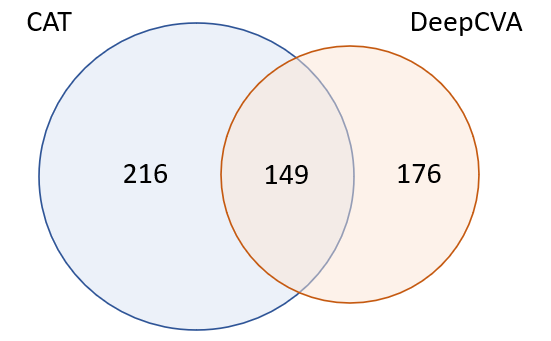
\includegraphics[width=1.65in]{graphs/Overlap-1.png}
		\vspace{-16pt}
		\caption{C Dataset}
		\label{RQ3-result-1}
	\end{subfigure}
	\begin{subfigure}{0.235\textwidth}
		\centering
		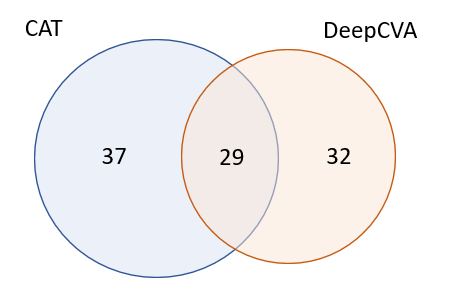
\includegraphics[width=1.65in]{graphs/Overlap-2.png}
		\vspace{-16pt}
		\caption{Java Dataset}
		\label{RQ3-result-2}
	\end{subfigure}
	\vspace{-6pt}
	\caption{Overlapping Analysis}
	\label{RQ3-result}
\end{figure}

Fig.~\ref{RQ3-result} shows the overlaps between the results from
{\tool} and DeepCVA. As seen, on the C dataset, {\tool} correctly
classified 216 commits (regarding all classes for VATs) that were
misclassified by DeepCVA. In contrast, DeepCVA correctly classified
176 commits that were misclassified by {\tool}. Both {\tool} and
DeepCVA correctly classified 149 commits. Moreover, on the Java
dataset, {\tool} can correctly classify 37 Java commits that were
misclassified by DeepCVA. In contrast, DeepCVA can correctly classify
32 Java commits that were misclassified by {\tool}. Both {\tool} and
DeepCVA correctly classified 29 Java commits. Note that the C dataset
(BigVul) is larger than the Java dataset (CVAD). BigVul has 7,851
commits with 785 commits for testing, while CVAD has 1,229 commits
with 123 commits for testing. Thus, the numbers in
Figs~\ref{RQ3-result-1} and~\ref{RQ3-result-2} are much different.
%Tien
%The rationale for choosing the CVAD dataset has two folds. First, we
%aim to compare {\tool} with DeepCVA, which used that dataset in their
%work. Second, we aim to evaluate {\tool} on Java vulnerabilities.


%Figure~\ref{RQ3-result} shows the results of overlapping analysis between {\tool} and DeepCVA on both C and Java datasets on average. On C dataset, {\tool} can correctly classify 2.1K+ C commits but missed by DeepCVA. DeepCVA can correctly classify 1.7K+ C commits but missed by {\tool}. Both {\tool} and DeepCVA can correctly classify 1.5K+ C commits. On Java dataset, {\tool} can correctly classify 37 Java commits but missed by DeepCVA. DeepCVA can correctly classify 32 Java commits but missed by {\tool}. Both {\tool} and DeepCVA can correctly classify 29 Java commits. On both datasets, {\tool} can correctly classify more commits than DeepCVA.




\subsection{\bf Ablation Study (RQ5)}

\input{sections/multi-task-table}

%		   \tool w/o Multi-task Learning       & 0.68  &  0.52    & 0.25         \\
%                    \tool with (VD $\rightarrow$ VA)   &  0.68      &   0.36   &  0.18  \\    
%                    \tool w/o Context                 & 0.75 &  0.57    & 0.29         \\

As seen in Tables~\ref{tab:impact-multi-task-on-detection}
and \ref{tab:impact-multi-task-on-assessment}, without multi-task
learning, the performance decreases 10.5\% F-score in detection and 15.6\%
macro F-score in assessment. Without context, it decreases 7.9\%
F-score in detection and 10.9\% macro F-score in assessment.
%We also built the model (VD $\rightarrow$ VA) in which the detection
%classifier is used first, and the assessment classifier is then used
%if the detection outcome is positive.
This result confirms our hypotheses:

(1) Multi-task learning helps improve both vulnerability detection and
assessment: adding multi-task learning, both VD and VA improve (0.68
to 0.76, 0.54 to 0.64). Note: without multi-task learning, {\tool}
also improves over the baselines
(Tables~\ref{tab:rq1}--~\ref{rq1_results}) in both VD and VA due to
{\tool}'s code change embeddings
(Section~\ref{sec:separation}).

%(2) Multi-task learning model performs much better than
%(VD $\rightarrow$ VA), which has the cascading error due to
%false positives in VD.

(2) both multi-task learning and context have positive contributions,
in which multi-task learning contributes more.

Multi-task learning model performs better than cascading VD to
VA, which has the cascading error due to false positives in VD.

%The corresponding decrease values for the model without Context are
%11.6\% F-score in detection and 10.9\% macro F-score in
%assessment. Thus, multi-task learning contributes more than
%context. We also built a model in which the detection classifier is
%applied first and if the result is positive (e.g., vulnerability), the
%classifiers for assessment will be used (i.e., VD $\rightarrow$ VA).
%As seen, the cascading error due to false positives reduce the
%performance significantly.



%As seen in Table~\ref{RQ4-result-1}, without~the context, the macro
%F-score and multi-class MCC decrease by 4.7\% and 6.1\%, respectively.
%Without the multi-task learning, the macro F-score and multi-class MCC
%decrease by 6.3\% and 9.1\%, respectively. While both the context and
%multi-task learning play positive roles in {\tool}'s accuracy,
%multi-task learning contributes slightly more.


%Table~\ref{RQ4-result-1} shows the overall macro-F-score and multi-class MCC results when the key features in {\tool} were removed. As seen in Table~\ref{RQ4-result-1}, without the context vector, the macro-F-score and multi-class MCC decrease by 4.7\% and 6.1\%, respectively. And without the multi-tasking framework, the macro-F-score and multi-class MCC decrease by 6.3\% and 9.1\%, respectively. While both context vector and the multi-tasking framework play a positive role in the overall performance, the multi-tasking framework contributes more to {\tool}.

\begin{table}[t]
	\caption{RQ5. Impact of Num. of Hops $k$ for Context Size}
	\vspace{-10pt}
	\begin{center}
%		\scriptsize
\small
		\tabcolsep 4pt
		\renewcommand{\arraystretch}{1} \begin{tabular}{p{3.5cm}<{\centering}|p{2cm}<{\centering}p{1.2cm}<{\centering}}
			
			\hline
			& macro F-Score & MCC \\ 
			\hline
			\tool ($k=1$)          & 0.62 & 0.32          \\
			\tool ($k=2$)          & 0.63 & 0.33          \\
			\tool ($k=3$)          & 0.64 & 0.33          \\
			\tool ($k=4$)          & 0.62 & 0.31          \\
			\tool ($k=5$)          & 0.61 & 0.30          \\
			\hline
		\end{tabular}
		\label{RQ4-result-2}
	\end{center}
\end{table}

Table~\ref{RQ4-result-2} shows the impact of the context size $k$ (the
number of hops from a changed node). As seen, when
%the context size
$k$ increases from 1--3, the macro F-score increases to its highest
value of 0.64.
%and the multi-class MCC increases to its highest value of 0.33.
However, when $k$ continues to increase $k \geq 3$, both macro F-score
and multi-class MCC decrease. The rationale is that as the context
size is too small, the limited number of surrounding nodes cannot
capture well the relevant statements for assessment. As the context size gets larger, the
increasing number of the irrelevant statements will bring in
biases. Thus, we selected $k$=3 in
other studies on the C dataset.

%Table~\ref{RQ4-result-2} shows the overall macro-F-score and multi-class MCC when we evaluate the size $K$ of a context (i.e., the number of hops from the changed node) on the C dataset. From the table, we can see that when the number of hops from the changed node increase from $K=1$ to $K=3$, the macro-F-score increases to its highest value $0.64$ and the multi-class MCC increases to its highest value $0.33$. But after $K=3$, with the rise of $K$ value, both macro-F-score and multi-class MCC decrease. The reason that causes this is that when the $K$ value is too small, the limited amount of surrounding nodes cannot capture all the relevant nodes well for \tool to learn the context information well. But if the $K$ value is too big, the increasing number of the irrelevant nodes will bring in too many biases and hurt the overall performance of \tool. Therefore, we select $K=3$ to be the best setting for \tool on our C dataset with this analysis.  















\iffalse

\begin{table}[h]
	\caption{Sensitive Analysis -- Impact of Different Factors on {\tool}'s Accuracy in terms of Top1 on BigFix Dataset. 
	%	Seq2seq: Simple Sequence to Sequence model; Two-Layer-EDM: Two Layers Tree-Based LSTM Encoder-Decoder Model; PAT: Program Analysis Techniques including Renaming and Program Analysis Filters.
	}
	\vspace{-10pt}
	\begin{center}
		\renewcommand{\arraystretch}{1} 
		\begin{tabular}{l|p{0.7cm}<{\centering}|p{1.5cm}<{\centering}}
			\hline
			Models & Top1 & Improvement\\
			\hline
			Seq2Seq & 1.8\% & \\
			Seq2Seq + PAT & 6.4\% & 256\% \\ 
			Two-Layer-EDM & 11.7\% & 550\%\\
			Two-Layer-EDM + PAT &  24.4\% &109\%\\
			Two-Layer-EDM + PAT + Re-ranking & 29.4\%&20.5\% \\
			\hline
		\end{tabular}
	Seq2seq: a simple sequence-to-sequence model; Two-Layer-EDM: Two-layer tree-based LSTM encoder-decoder model; 
	PAT: program analysis (PA) Techniques including Renaming and PA Filters.
		\label{RQ3}
	\end{center}
%\vspace{-10pt}
\end{table}

%We conducted an experiment to study how different factors including renaming, two Layer encoder-decoder model, models for encoders and decoders, program analysis filters, re-selecting model affect our model's accuracy.

Table~\ref{RQ3} shows that we build three variants of {\tool} with
different factors and their combinations.  We analyze our results as
follows:

(1) \textbf{Impact of Two-Layer-EDM}. Our Two-Layer-EDM
can improve the one-layer sequence-to-sequence model by 550\% and
using only {\em seq2seq} cannot get good results. Two-layer-EDM is
designed to learn the local context of a bug fix and code
transformations.

(2) \textbf{Impact of PAT}. Using program analysis (PA) techniques,
PAT, including alpha-renaming and PA-filtering, is effective to
improve Two-Layer-EDM by 109\%.
%This is reasonable because the program analysis techniques can make our data become more common in order to make the training data can contribute more and also can help reduce the wrong candidate patch by program analysis filters to reduce the search space and increase the accuracy.
The alpha-renaming process can help improve {\tool} for better training
and the PA-filtering process can help elminate more the irrelevant patches.
%From \textit{Seq2seq} in Table~\ref{RQ3}, we can see that by only using one layer simple seq2seq model to do the bug fix cannot get a good result on BigFix.
%To study the impact of our two layers tree-based encoder decoder model, we compare the results obtained from two variants: \textit{Seq2seq} and \textit{TLTM}. The results show that using the our two layers tree-based encoder decoder model can increase accuracy relatively by 550\%. This is because TLTM can analysis local context and code transformation at the same time with less biases.

Adding program analysis to the basic {\em seq2seq} model can improve
it by 256\%. However, the Two-Layer-EDM can improve seq2seq by 550\%.
Thus, the Two-Layer-EDM has more impact than PAT.

(3) \textbf{Impact of Re-ranking}. The results
of \textit{Two-Layer-EDM + PAT + Re-Ranking} show that having
re-ranking can increase accuracy relatively by 20.5\%. The reason is
that the re-ranking process, which uses a Convolutional Layer to
distinguish the best result from the others, can help increase
{\tool}'s accuracy by pushing the right results to the top of the list
of the candidate fixes.

\fi

%The re-ranking part which uses convolutional layer to classify the
%best result and other results can help increase the accuracy of our
%approach. In this way, the re-ranking can help our approach a lot.
%The Re-ranking can improve the model with Two-layer-EDM + PAT by
%20.5\%. The results show that once the model generates a list of
%candidate patches, re-ranking the list can help improve the results.

\subsubsection{\bf Comparative Study on Java Dataset (RQ6)}

\begin{table}[t]
	\caption{RQ6. Performance on Java Dataset}
        \vspace{-9pt}
	\begin{center}
        \tabcolsep 2.5pt
%		\footnotesize
\small
		\renewcommand{\arraystretch}{1}
		\begin{tabular}{l|p{2.0cm}<{\centering}|p{1.6cm}<{\centering}|p{1.5cm}<{\centering}}
			\hline
			\multirow{2}{*}{CVSS Metric}     & \multirow{2}{*}{Evaluation Metric}  & \multicolumn{2}{c}{Model}\\
			\cline{3-4}
			&                                     & DeepCVA    & \tool       \\
			\hline
			\multirow{2}{*}{Confidentiality} & macro F1-score                             &     0.44       & 0.55\\
			\cline{2-4}
			& MCC                                 &      0.27      & 0.32\\
			\hline
			\multirow{2}{*}{Integrity}       & macro F1-score                             &    0.43        & 0.52\\
			\cline{2-4}
			& MCC                                 &    0.25        & 0.27\\
			\hline
			\multirow{2}{*}{Availability}    & macro F1-score                             &   0.43         & 0.54\\
			\cline{2-4}
			& MCC                                 &    0.27        & 0.27\\
			\hline
			\multirow{2}{*}{Access Vector}   & macro F1-score                             &   0.55         & 0.59\\
			\cline{2-4}
			& MCC                                 &    0.13        & 0.17\\
			\hline
			\multirow{2}{*}{Access Complexity} & macro F1-score                           &   0.46         & 0.53\\
			\cline{2-4}
			& MCC                                 &    0.24        & 0.26\\
			\hline
			\multirow{2}{*}{Authentication}  & macro F1-score                             &   0.66         & 0.68\\
			\cline{2-4}
			& MCC                                 &   0.35         & 0.38\\
			\hline
			\multirow{2}{*}{Severity}        & macro F1-score                             &   0.42         & 0.51\\
			\cline{2-4}
			& MCC                                 &   0.21         & 0.22\\
			\hline
			\hline
			\multirow{2}{*}{Average}         & macro F1-score                             &    0.45        & 0.59 ($\Uparrow${\bf 31.0\%})\\
			\cline{2-4}
			& MCC                                 & 0.24           & 0.32 ($\Uparrow${\bf 33.3\%})\\
			\hline
                        \hline
\multirow{2}{*}{Vulnerability Detection} &  & VCCFinder & CAT \\
\cline{2-4}
 & F-score & 0.24 & 0.76 \\
\hline
		\end{tabular}
		\label{rq2_results}
	\end{center}
\end{table}

We aim to show that our approach also works for vulnerability in a
different programming language. Table~\ref{rq2_results} shows that it relatively
improves DeepCVA~\cite{deepCVA-ase21} by {\em 31.0\% in macro F1-score
and 33.3\% in multi-class MCC} on the overall multi-class
classification in Java dataset. For specific VATs, {\tool} improves
DeepCVA by {\em 3.0--25.6\% in macro-F1-score and 30.8\% in
multi-class MCC}. Moreover, the largest relative improvement in macro
F1-score happens for {\em Availability} and the largest one in
multi-class MCC happens for {\em Access Vector}.
%The lowest relative improvement in both macro F1-score and
%multi-class MCC happens for {\em Authentication}, however,
The absolute macro F1-score value (0.68) for {\em Authentication} is
highest among all the VATs.
%
The F-score for detection from {\tool} is also higher than that of the
commit-level VCCFinder, which uses SVM. Other baselines in
Table~\ref{tab:rq1} do not work on Java code. In brief, this result is
consistent with the trend as {\tool} being run on the C dataset.


%Thus, {\tool}'s assessment works for Java.

%Table~\ref{rq2_results} shows that {\tool} outperforms the state-of-the-art baseline, DeepCVA, in the automation of commit-level vulnerability assessment on the Java dataset. Particularly, {\tool} improves the state-of-the-art baseline by 14.3\% in terms of macro-F1-score, and 8.0\% in terms of multi-class MCC on the overall performance. The higher values of macro-F1-score and MCC indicate that {\tool} can perform more accurate multi-classification on Java commits than DeepCVA. As for specific types of vulnerability assessment, {\tool} improves the state-of-the-art baseline by 3.0-25.6\% in terms of macro-F1-score and 0-30.8\% in terms of macro-F1-score. The lowest relative improvement of both macro-F1-score happens when testing the $Authentication$. And when testing $Availability$, \tool and DeepCVA get the same multi-class MCC. As for the biggest relative improvement, when testing $Availability$, \tool achieves the biggest relative improvement on the macro-F1-score, and the biggest relative improvement of multi-class MCC happens when testing $Access Vector$.































%%\subsection{Discussion and Implications}

%\subsubsection{Using Explainable AI to explain the graph as the key features in {\tool}}

\subsubsection{{\bf Using Explainable AI for Study Relevant Features in Classification regarding Program Dependencies (RQ4)}}
\label{discuss:sec}

%\subsubsection*{Using Explainable AI to explain the graph as the key features in {\tool}}

%{\tool} has two key ideas (Section~\ref{key-ideas:sec}) in advancing
%the state-of-the-art commit-level vulnerability assessment: 1)
%graph-based code change representation learning for program
%dependencies; and 2) contextualized embeddings for code changes. As
%seen in RQ5, our context-aware, graph-based, representation learning
%(RL) model produces the embeddings for the code changes in the
%commits that facilitate {\tool} in better classifying the
%commit-level changes into more correct classes regarding  the assessment
%types than DeepCVA~\cite{deepCVA-ase21}.
We aim to show that {\tool} in fact leverages the
program dependencies among statements in its vulnerability
assessment.
%capable of {\em capturing the key vulnerable statements and
%dependencies}, leading to its accuracy in vulnerability assessment.
Specifically, for each vulnerability assessment type (VAT) (e.g., {\em
Availability}), we randomly selected 366 samples of the commits in our
C dataset that {\tool} predicts the correct classes (e.g., {\em None},
{\em Partial}, or {\em Complete}) of the vulnerability detection and
VATs for those commits. That sample size gives us the confidence
level of 95\% and the confidence interval of 5\% for each VAT.

We use an explainable Artificial Intelligence (XAI) model,
called {\em GNNExplainer}~\cite{GNNExplainer}, which takes a GNN-based
classification model $\mathcal{M}$ and a specific input $I$ of
$\mathcal{M}$, and produces an explanation on why $\mathcal{M}$
arrives at its prediction $O$ for the input $I$.
%
We fed {\tool} and each commit $C$ of those sample commits as the
input for GNNExplainer. The explanation produced by GNNExplainer is in
the form of a sub-graph $\Delta$ in {\mvpdg} that was built from the
input commit $C$. The sub-graph $\Delta$ is referred to as the {\em
explanation sub-graph} for $C$ regarding the classification of $C$ for
the current assessment type. The explanation sub-graph $\Delta$ is
defined as the minimal sub-graph in the input graph {\mvpdg} that
minimizes the prediction scores between using the entire graph
{\mvpdg} and using $\Delta$ as the input for {\tool}. $\Delta$ is
minimal in the sense that if any node and edge is removed from it, the
decision of {\tool} is affected, i.e., {\tool} will produce a
different class for the input commit $C$. That is, {\em the
explanation sub-graph $\Delta$ contains the statements and
dependencies that are most decisive for {\tool} to determine the class
$O$ for the commit $C$}.

To evaluate whether {\tool} via Label-GCN can capture the crucial
statements and dependencies in deciding the class for an input commit,
%regarding an assessment type,
we compared the explanation sub-graph $\Delta$ with the
vulnerability-introducing statements and dependencies in the ground
truth of those commits. If $\Delta$ contains one of such statements
(nodes) and dependencies (edges), we consider that {\tool} uses the
correct vulnerable statements and dependencies as the features for its
correct classification (detection and assessment).
%regarding an assessment type.

%\textcolor{red}{As seen in Table~\ref{},...}

\begin{table}[t]
\caption{Vunerable Statements/Dependencies as Key Features}
	\vspace{-7pt}
	\tabcolsep 2.1pt
%	\footnotesize
\small
	\begin{center}
\begin{tabular}{|r||r|r|r|r|r|r|r||r|}
  \hline
    {\bf VulDet} & {\em Confi} & {\em Integ.} & {\em Avail} & {\em AccessVec} & {\em AccCompl} & {\em Auth} & {\em Severity} & {\bf Avg} \\
  \hline
  {\bf 84} & 63 & 84 & 81 & 72 & 93 & 93 & 81 & 81.4 \\
 % \% & 17 & 22 & 11 & 19 & 24.5 & 37 & 21 & 21.6 \\
  \hline
\end{tabular}
\label{gnn}
\%Commits {\tool} correctly uses vulnerable statements/dependencies in Vulnerability Detection and Assessment
\end{center}
\vspace{-3pt}
\end{table}

%N= \# of commits that \tool correctly uses the vulnerable statements and dependencies\\

%Table~\ref{gnn} shows us how much {\tool} uses the vulnerable statements and their dependencies in predicting the correct assessments. For example, among a sample of 366 commits that {\tool} successfully classified into {\em None} or {\em Single} for {\em Authentication}, there are 139 commits in which {\tool} uses the actual vulnerable statements and their dependencies in its prediction/assessment. GNNExplainer determines that {\tool} had made the correct classifications for {\em Authentication} because {\tool} used at least one of the actual vulnerable statements/dependencies. In other words, in 139 commits, {\tool} used the vulnerable statements/dependencies as its key features in the correct classifications. As seen, across different assessment types, the degree of {\tool}'s relying on the vulnerable statements and dependencies for its assessment is different. While only 11\% of the samples, {\tool} relies on vulnerable statements/dependencies to assess the impact of {\em Availability}, in 37\% of the samples, it relies on them for assessing that of {\em Authentication}. On average, in 21.6\% of the samples, {\tool} correctly relies on the vulnerable statements and their dependencies in vulnerability assessment. 

Table~\ref{gnn} shows how much {\tool} uses the vulnerable
statements and their dependencies in correctly predicting the
VATs. For example, among 366 commits that {\tool} successfully
classified into ({\em None},{\em Single}) for {\em Authentication},
GNNExplainer determines 93\% of them that {\tool}
uses the actual vulnerable statements and their dependencies as key
features in its prediction.
%GNNExplainer determines that {\tool} had made the correct
%classifications for {\em Authentication} because {\tool} used at least
%one of the actual vulnerable statements/dependencies.
%That is, in 139 commits, {\tool} used the vulnerable
%statements/dependencies as its key features in the correct
%classifications.
As seen, across different assessment types, the degree of {\tool}'s
relying on the vulnerable statements/dependencies for its assessment
is different.  While in 84\%, {\tool} relies on vulnerable
statements/dependencies to assess the impact of {\em Integrity}, in 81\% samples, it relies on them for assessing that of {\em Severity}.
For vulnerability detection, 84\% of samples, {\tool} uses
the right statements/dependencies in its correct prediction.
%
On average, in 81.4\% samples per assessment type, {\tool} correctly
relies on the vulnerable statements/dependencies in its assessment.
%To correctly assess the remaining samples, {\tool} might use other
%features, e.g., contexts, code tokens, and the impacts of
%multiple~tasks.
In brief, this result shows that {\em program dependencies among
vulnerable statements are key features to {\tool} in its correct
vulnerability detection and assessment}.



%In the other 78.4\%, {\tool} uses other features for correct classifications. Even though the vulnerability-introducing statements and dependencies are not in the minimum sub-graphs from GNNExplainer. However, we found that in all of the 78.4\% cases, one or several statements in the minimum sub-graphs have direct dependencies with the vulnerability-introducing statements. 
%(but they are not directly connected). %The reason is that GNNExplainer, an approximation explanation model, is limited in generating only connected graphs as explanations, thus if the contributing features are a combination of a connected graph and a couple non-connected statements, then the non-connected ones will not be included in the sub-graphs. 




%automatic verification of 

%We can only automatically verify whether {\tool} reasons over actual vulnerable statements and their dependencies using vulnerable statements and dependencies. We also further analyze the other 78.4\% cases. In the other 78.4\%, {\tool} uses other features for correct classifications, such as combinations of 



%As seen in Table~\ref{discussion}, we use the confidence level of 95\% and the confidence interval of 5\% to pick out a sample dataset to do the analysis. By running the GNNExplainer for every task, \tool can correctly use the vulnerable statements and dependencies as the features for 41-139 cases among 379 vulnerability introducing commits that \tool correctly classified (Each vulnerability assessment type may have different 379 vulnerability introducing commits). When running GNNExplainer on $Authentication$, the number of cases that \tool can correctly use the vulnerable statements and dependencies is the biggest among seven vulnerability assessment types. And when running GNNExplainer on $Availability$, the number of cases that \tool can correctly use the vulnerable statements and dependencies is the smallest one among seven vulnerability assessment types. On average, \tool can correctly use the vulnerable statements and dependencies as the features for 81.9 cases among 379 vulnerability introducing commit.


%\begin{table}[t]
%	\caption{GNNExplainer Running Results}
%	\vspace{-9pt}
%	\begin{center}
%		\footnotesize
%		\renewcommand{\arraystretch}{1}
%		\begin{tabular}{p{2cm}<{\centering}|p{4cm}<{\centering}}
%			\hline
%			                                  & \# of commits that \tool correctly uses the vulnerable statements and dependencies       \\
%			\hline
%			Confidentiality                   & 63                  %        \\
%			\hline
%			Integrity                         & 84                  %         \\  
%			\hline
%			Availability                      & 41                  %                    \\
%			\hline
%			Access Vector                     & 72                  %          \\
%			\hline
%			Access Complexity                 & 93                  %          \\
%			\hline
%			Authentication                    & 139                 %           \\
%			\hline
%			Severity                          & 81                  %         \\
%			\hline  
%			\hline
%			Average                           & 81.9                %         \\
%			\hline
%		\end{tabular}
%		\label{discussion}
%	\end{center}
%\end{table}



%\subsubsection*{Illustrating Example}

\begin{figure}[t]
\centering
\lstset{
      		numbers=left,
		numberstyle= \tiny,
		keywordstyle= \color{blue!70},
		commentstyle= \color{red!50!green!50!blue!50},
		frame=shadowbox,
		rulesepcolor= \color{red!20!green!20!blue!20} ,
		xleftmargin=1.5em,xrightmargin=0em, aboveskip=1em,
		framexleftmargin=1.5em,
                numbersep= 5pt,
		language=Java,
                basicstyle=\scriptsize\ttfamily,
                numberstyle=\scriptsize\ttfamily,
                emphstyle=\bfseries,
                moredelim=**[is][\color{red}]{@}{@},
		escapeinside= {(*@}{@*)}
	}
	\begin{lstlisting}[]
private: Status DoCompute(OpKernelContext* ctx) { ...
(*@{\color{purple}{\fbox{+ DatasetBase* finalized\_dataset;}}}@*)
(*@{\color{violet}{\fbox{+ TF\_RETURN\_IF\_ERROR(FinalizeDataset(ctx, dataset, \&finalized\_dataset));}}}@*)
  std::unique_ptr<IteratorBase> iterator;
(*@{\color{black}{- TF\_RETURN\_IF\_ERROR(}@*)(*@{\color{black}{dataset}@*)(*@{\color{black}{->MakeIterator(\&iter\_ctx,/*parent=*/nullptr,.));}}@*)
(*@{\color{violet}{\fbox{+ TF\_RETURN\_IF\_ERROR(finalized\_dataset->MakeIterator(\&iter\_ctx,/*parent=*.));}}}@*)
  std::vector<Tensor> components;
(*@{\color{black}{- components.reserve(}@*)(*@{\color{black}{dataset}@*)(*@{\color{black}{->output\_dtypes().size());}}@*)
(*@{\color{red}{\fbox{+ components.reserve(finalized\_dataset->output\_dtypes().size());}}}@*) ...
}
\end{lstlisting}
\vspace{-19pt}
\caption{Contributions of different statements in correct
vulnerability prediction and classification of VATs by {\tool}}
\vspace{-4pt}
\label{gnn-example}
\end{figure}

%/*parent=*/nullptr,.));

%{\color{red}{ CVSS Score -> 4.6

%$Severity$ -> Medium

%GNNExplainer Sub-graph (6 Nodes)-> Line 5, 6, 10, 12, 14, one line not shown in the example.}}

\vspace{3pt}
\noindent {\bf Example.} Figure~\ref{gnn-example} shows an example of
the vulnerability-introduc\-ing change for CVE-2021-37650. The change
introduced the variable \code{finalized\_dataset} at line 2,
representing a dataset that was populated at line 3 and used at lines
6 and 9. However, the input was not validated, and the code at line 9
assumed only string inputs and interpreted numbers as valid strings.
When computing the CRC of the record, this resulted in~heap buffer
overflow. {\tool} correctly~predicted this vulnerability and its
assessment {\em Severity=Medium}. GNNExplainer pointed out that
{\tool} used the changed statements and their dependencies at lines 2,
3, 6, 9 and another line (not shown), to perform classification. This
is correct because despite~line~9 being a fixed line (in a later
version), lines 2, 3, 6 are parts of the control/data flows leading to
line 9. Thus, {\tool} correctly used the vulnerability-relevant
statements and dependencies in correct~prediction.

%Thus, program dependencies encoded in our embeddings are the
%key features enabling {\tool} in correct classification.


%Tien
%Thus, {\tool} correctly used the statements/dependencies as the key
%features in its assessment. That is, our graph representations with
%program dependencies encoded by the embeddings have positive
%contributions to {\tool}'s accuracy.


%Code assumes only strings inputs and then interprets numbers as valid
%`tstring`s. Then, when trying to compute the CRC of the record this
%results in heap buffer overflow.


%private:
%Status DoCompute(OpKernelContext* ctx) {
%	...
%	IteratorContext iter_ctx(std::move(params));
%(*@{\color{cyan}{+ \quad	DatasetBase* finalized\_dataset;}}@*)
%(*@{\color{cyan}{+ \quad	TF\_RETURN\_IF\_ERROR(FinalizeDataset(ctx, dataset, \&finalized\_dataset));}}@*)
	
%	std::unique_ptr<IteratorBase> iterator;
%(*@{\color{red}{-	\quad   TF\_RETURN\_IF\_ERROR(dataset->MakeIterator(\&iter\_ctx, /*parent=*/nullptr, "ToTFRecordOpIterator", \&iterator));}}@*)
%(*@{\color{cyan}{+	\quad   TF\_RETURN\_IF\_ERROR(finalized\_dataset->MakeIterator(\&iter\_ctx, /*parent=*/nullptr, "ToTFRecordOpIterator", \&iterator));}}@*)
	
%	std::vector<Tensor> components;
%(*@{\color{red}{- \quad	components.reserve(dataset->output\_dtypes().size());}}@*)
%(*@{\color{cyan}{+ \quad	components.reserve(finalized\_dataset->output\_dtypes().size());}}@*)
%	bool end_of_sequence;
%	...
%}



\subsubsection{Threats to Validity}
The threats come from the following aspects: (1) \emph{Programming languages (PLs).}  Our approach has been tested on
Java and C commits. However, the techniques used in {\tool} are not
tied to Java or C.  In principle, our approach can applied to other PLs. (2) \emph{Generalization of the results.}  Our comparisons with
DeepCVA were only carried out on the C and Java datasets that are both publicly available.  Further validation of the comparisons with DeepCVA on other datasets should be done in future. 
%(3) \textbf{Training and Tuning.} It is impossible to test the entire hyperparameter space. However, on the Java dataset (used by DeepCVA), we reused the parameters reported in DeepCVA for training and tuning. On the C dataset, 





\section{Related Work}

%Here, we summarize some studies relevant to our study.

\noindent{\bf Automated Vulnerability Assessment. }
Distinct software vulnerabilities can have different levels of threats
and severity~\cite{nayak2014some,le2019automated}. Thus, it is desired
to assess vulnerabilities for prioritizing actions and resources
%so that more severe ones can be studied and patched
before more exploits~\cite{khan2018review}.  The automated approaches
have been recently
proposed~\cite{bozorgi2010beyond,allodi2014comparing,deepCVA-ase21}.
Bozorgi {\em et al.}~\cite{bozorgi2010beyond} proposed a SVM-based
approach to predict whether a vulnerability will be exploited or
not.
%Specifically, they extracted over 93k features from vulnerability data
%and classify vulnerabilities using these features.
This work represents the early effort to replace the small-scale
rating-based assessment framework by learning-based approaches.
Lamkanfi {\em et al.}~\cite{lamkanfi2010predicting} predict the
severity of a reported bug using text mining algorithms to analyze the
textual descriptions on the bugs.
%
Han {\em et al.}~\cite{han2017learning} proposed a multi-class text
classification DL-based model that is based on the
description to predict the severity level of a vulnerability.
%critical, high, medium, and low in CVSS~\cite{first-website}.

%Specifically, given a vulnerability description, they classified the
%text into one of the severity levels, for example, critical, high,
%medium, low of the Common Vulnerability Scoring System (CVSS)
%framework~\cite{first-website}.
Georgios {\em et al.}~\cite{spanos2018multi} adopted a multi-target
classification approach coupled with text analysis on vulnerability
descriptions to predict the vulnerability characteristics and scores.
Le {\em et al.}~\cite{le2019automated} proposed a ML-based approach to
not only learn the word features in vulnerability description, but
also handle the new or extended concepts in the new vulnerability's
description. Unlike the above studies built for analyzing
vulnerability description, some other
studies~\cite{ponta2018beyond,ponta2020detection} leveraged code
patterns in fixing commits of third-party libraries to assess
vulnerabilities in such libraries. In comparison, {\tool} is
fundamentally different from the above studies, as it supports
commit-level vulnerability assessment using code changes.

%{\tool} is closely related to DeepCVA as explained in
%Section~\ref{intro:sec}.

%The most relevant work to {\tool} is the state-of-the-art commit-level approach, DeepCVA, working on code changes. However, {\tool} is designed to overcome the shortcomings of DeepCVA in code change representation and embeddings, program dependencies and surrounding contexts of changed code. Our empirical studies have shown that {\tool} can outperform DeepCVA.

\vspace{3pt}
\noindent{\bf Vulnerability Prediction. }
%Commit-level vulnerability detection is an important direction.
Commit-level vulnerability detection is
important~\cite{perl2015vccfinder,zhou2017automated,chen2019large}.
%developed commit-level VD models that leveraged ML models.
VCCFinder~\cite{perl2015vccfinder} trained a SVM classifier to flag
suspicious commits. We used only code change features for our
experiment. Zhou and Sarma~\cite{zhou2017automated} work on commit
messages and bug reports, It uses an ensemble approach to combine
multiple classifiers.
%with random forest,
%gaussian naive bayes, k-nearest neighbors, SVM, etc.
%Many studies (e.g, \cite{li2021vulnerability,
%  zhou2019devign,li2021vuldeelocator,li2020automated,chakraborty2021deep,hin2022linevd})
%also built machine or deep learning models to detect vulnerabilities
%in source code.
However, {\tool} also supports vulnerability assessment together with
detection.
%Their tools are not publicly available for comparison. We expect that
%deep learning models would perform better than classic ML classifiers.

%is apart from them, as we focused on
%vulnerability assessment that is as important as detection.

Deep learning (DL) has been applied
to detect
vulnerabilities~\cite{li2021vulnerability,zhou2019devign,li2021vuldeelocator,li2020automated,chakraborty2021deep,hin2022linevd,scandariato2014predicting,neuhaus2007predicting,shin2010evaluating,neuhaus2009beauty,yamaguchi2012generalized,yamaguchi2011vulnerability}.
%For example, some approaches train a DL model on different code
%representations to detect vulnerabilities, such as the lexical
%representations of functions in a synthetic
%codebase~\cite{harer2018learning}, code snippets related to API calls
%to detect two types of vulnerabilities~\cite{li2018vuldeepecker},
%syntax-based, semantics-based, and vector
%representations~\cite{li2018sysevr}, graph-based
%representations~\cite{zhou2019devign}.
Harer {\em et al.}~\cite{harer2018learning} train an RNN to detect
vulnerabilities. Lin {\em et al.}~\cite{lin2017poster} automatically
learns high-level representations of functions based on AST for
VD. Russell {\em et al.}~\cite{russell2018automated} combine the
neural feature representations of functions with random forest as a
classifier.
%It does not consider program dependencies.
Harer {\em et al.}~\cite{harer2018automated} compared the
effectiveness in VD of using source code and the compiled
code. VulDeePecker~\cite{li2018vuldeepecker} uses a RNN trained on
program slices from API calls for VD. SySeVR~\cite{li2021sysevr}
expands VulDeePecker by including the program slices from more
syntactic units: arrays, pointers, and arithmetic expressions.
Devign~\cite{zhou2019devign} uses Gated Graph Recurrent Layers on CPG,
PDG, CFG, AST and code sequences. Reveal~\cite{chakraborty2020deep}
uses CPG with GGNN. IVDetect~\cite{li2021vulnerability} focuses on
interpretation and directly uses PDG with
GCN. LineVul~\cite{linevul-msr22} use BigVul dataset to train a
transformer-based model which has over 150K training instances. To
avoid under-training of LineVul and an unfair comparison (given that
it has over 110M parameters), we chose to not compare with it.
%Assessment is the key for earlier prioritization and resource
%relocation for identified vulnerabilities. Furthermore, detection
%models can be used to help detect vulnerabilities and then {\tool}
%assesses them.

Our work is also related to code change embedding
approaches~\cite{cc2vec,commit2vec}. Those approaches mainly treat
code as sequences and do not consider structures and/or program
dependencies. The key departure points of {\tool} from those
approaches include the use of graph representation to model the
changes and dependencies, as well as the surrounding context to build
the embeddings.



%\noindent{\bf Code Embedding Learning.}




\section{Conclusion}

This paper proposes {\tool}, a Context-aware, Graph-based,
Commit-level Vulnerability Detection and Assessment Model that
evaluates a commit, and detect any vulnerability and provides the CVSS
assessment grades for the detected vulnerability. The key advances in
{\tool} over the state-of-the-art commit-level approaches include 1)
multi-task learning between vulnerability detection and assessments of
different aspects, 2) code change embedding model that integrates
program dependencies and contexts, and 3) explicit graph-based
representations of depedencies and contexts. Our evaluation shows that
on a vulnerability dataset in C, CAT achieves F-score of 25.5\% and
MCC of 26.9\% relatively higher than the baseline in vulnerability
assessment. In Java dataset, CAT achieves F-score of 31\% and MCC of
33.3\% relatively higher. Our contextualized embeddings have other
applications related to code changes.

%(1) Integrating program dependencies into our commit-level
%vulnerability assessment approach; (2) Learning contexualized
%embeddings for code changes that integrating program dependencies
%among the program elements and the contexts of code changes.



%We propose a new context-aware, graph-based, commit-level vulnerability assessment approach, namely {\tool} to improve the most state-of-the-art commit-level vulnerability assessment approach, DeepCVA. The key ideas that enable our approach are (1) Integrating program dependencies into our commit-level vulnerability assessment approach; (2) Learning contexualized embeddings for code changes that integrating program dependencies among the program elements and the contexts of code changes. In our {\tool}, we leverage and train the Label, Graph Convolution Network (Label-GCN) to learn the program dependencies among the changed code and its surrounding unchanged code to generate the contextualized embeddings for code changes in the automated assessment of the vulnerability assessment types.

%We have conducted extensive empirical studies to evaluate {\tool} on two different datasets in C and Java. {\tool} is able to outperform the most recent and state-of-the-art automated vulnerability assessment approach, DeepCVA. Particularly, on the C dataset, {\tool} can improve DeepCVA by xx\% and xx\% in terms of F1-score and MCC, respectively. On the Java dataset, {\tool} can improve DeepCVA by xx\% and xx\% in terms of F1-score and MCC, respectively. Furthermore, our sensitivity analysis shows that all designed components of {\tool} can positively contribute to the model.





 %Designing a context-aware, graph-based, representation learning model to learn the contextualized embeddings for the code changes.










\newpage

\balance

%\bibliographystyle{plain}
%\bibliographystyle{ACM-Reference-Format}
\bibliographystyle{ACM-Reference-Format}

\bibliography{References,icse23}

\end{document}
